% **************************************************
% Document Class Definition
% **************************************************
\documentclass[%
	paper=A4,					% paper size --> A4 is default in Germany
	twoside=true,				% onesite or twoside printing
	openright,			.
	% doublepage cleaning ends up right side
	parskip=full,				% spacing value / method for paragraphs
	chapterprefix=true,			% prefix for chapter marks
	11pt,						% font size
	headings=normal,			% size of headings
	bibliography=totoc,			% include bib in toc
	listof=totoc,				% include listof entries in toc
	titlepage=on,				% own page for each title page
	captions=tableabove,		% display table captions above the float env
	draft=false,				% value for draft version
]{scrreprt}%

% **************************************************
% Debug LaTeX Information
% **************************************************
%\listfiles

% **************************************************
% Information and Commands for Reuse
% **************************************************
\newcommand{\thesisTitle}{Thesis Title}
\newcommand{\thesisName}{Alessio Rocchi}
\newcommand{\thesisSubject}{Thesis Subject}
\newcommand{\thesisDate}{11 November, 2015}
\newcommand{\thesisVersion}{Draft}

\newcommand{\thesisFirstReviewer}{Nikos G. Tsagarakis}
\newcommand{\thesisFirstReviewerUniversity}{\protect{Istituto Italiano di Tecnologia}}
\newcommand{\thesisFirstReviewerDepartment}{Advanced Robotics Department}

\newcommand{\thesisSecondReviewer}{Antonio Bicchi}
\newcommand{\thesisSecondReviewerUniversity}{\protect{Universit\`a di Pisa}}
\newcommand{\thesisSecondReviewerDepartment}{Centro E. Piaggio}

\newcommand{\thesisFirstSupervisor}{Nikos G. Tsagarakis}
\newcommand{\thesisSecondSupervisor}{Antonio Bicchi}

\newcommand{\thesisUniversity}{\protect{Universit\`a di Genova}}
\newcommand{\thesisUniversityDepartment}{Advanced Robotics Department}
\newcommand{\thesisUniversityInstitute}{Istituto Italiano di Tecnologia}
\newcommand{\thesisUniversityGroup}{Clean Thesis Group (CTG)}
\newcommand{\thesisUniversityCity}{Genova}
\newcommand{\thesisUniversityStreetAddress}{via Morego 30}
\newcommand{\thesisUniversityPostalCode}{16163}

% **************************************************
% Load and Configure Packages
% **************************************************
\usepackage[utf8]{inputenc}		% defines file's character encoding
\usepackage[english]{babel} % babel system, adjust the language of the content
\usepackage[					% clean thesis style
	figuresep=colon,%
	sansserif=false,%
	hangfigurecaption=false,%
	hangsection=true,%
	hangsubsection=true,%
	colorize=full,%
	colortheme=bluemagenta,%
	bibsys=bibtex,%
	bibfile={bib/refs},%
	bibstyle=alphabetic,%
]{cleanthesis}
\usepackage{amsmath}
\usepackage[toc,page]{appendix}
\usepackage{rotating}

\hypersetup{					% setup the hyperref-package options
	pdftitle={\thesisTitle},	% 	- title (PDF meta)
	pdfsubject={\thesisSubject},% 	- subject (PDF meta)
	pdfauthor={\thesisName},	% 	- author (PDF meta)
	plainpages=false,			% 	-
	colorlinks=false,			% 	- colorize links?
	pdfborder={0 0 0},			% 	-
	breaklinks=true,			% 	- allow line break inside links
	bookmarksnumbered=true,		%
	bookmarksopen=true			%
}

% **************************************************
% Document CONTENT
% **************************************************
\begin{document}

% --------------------------
% rename document parts
% --------------------------
%\renewcaptionname{ngerman}{\figurename}{Abb.}
%\renewcaptionname{ngerman}{\tablename}{Tab.}
\renewcaptionname{english}{\figurename}{Fig.}
\renewcaptionname{english}{\tablename}{Tab.}

% --------------------------
% Front matter
% --------------------------
\pagenumbering{roman}			% roman page numbing (invisible for empty page style)
\pagestyle{empty}				% no header or footers
% !TEX root = ../thesis-example.tex
%
% ------------------------------------  --> cover title page
\begin{titlepage}
	\pdfbookmark[0]{Cover}{Cover}
	\flushright
	\hfill
	\vfill
	{\LARGE\thesisTitle \par}
	\rule[5pt]{\textwidth}{.4pt} \par
	{\Large\thesisName}
	\vfill
	\textit{\large\thesisDate} \\
	Version: \thesisVersion
\end{titlepage}


% ------------------------------------  --> main title page
\begin{titlepage}
	\pdfbookmark[0]{Titlepage}{Titlepage}
	\tgherosfont
	\centering

	{\Large \thesisUniversity} \\[4mm]
	
\includegraphics[width=6cm]{gfx/Clean-Thesis-Logo} \\[2mm]
	\textsf{\thesisUniversityDepartment} \\
	\textsf{\thesisUniversityInstitute} \\
	\textsf{\thesisUniversityGroup} \\

	\vfill
	{\large \thesisSubject} \\[5mm]
	{\LARGE \color{ctcolortitle}\textbf{\thesisTitle} \\[10mm]}
	{\Large \thesisName} \\

	\vfill
	\begin{minipage}[t]{.27\textwidth}
		\raggedleft
		\textit{1. Reviewer}
	\end{minipage}
	\hspace*{15pt}
	\begin{minipage}[t]{.65\textwidth}
		{\Large \thesisFirstReviewer} \\
	  	{\small \thesisFirstReviewerDepartment} \\[-1mm]
		{\small \thesisFirstReviewerUniversity}
	\end{minipage} \\[5mm]
	\begin{minipage}[t]{.27\textwidth}
		\raggedleft
		\textit{2. Reviewer}
	\end{minipage}
	\hspace*{15pt}
	\begin{minipage}[t]{.65\textwidth}
		{\Large \thesisSecondReviewer} \\
	  	{\small \thesisSecondReviewerDepartment} \\[-1mm]
		{\small \thesisSecondReviewerUniversity}
	\end{minipage} \\[10mm]
	\begin{minipage}[t]{.27\textwidth}
		\raggedleft
		\textit{Supervisors}
	\end{minipage}
	\hspace*{15pt}
	\begin{minipage}[t]{.65\textwidth}
		\thesisFirstSupervisor\ and \thesisSecondSupervisor
	\end{minipage} \\[10mm]

	\thesisDate \\

\end{titlepage}


% ------------------------------------  --> lower title back for single page layout
\hfill
\vfill
{
	\small
	\textbf{\thesisName} \\
	\textit{\thesisTitle} \\
	\thesisSubject, \thesisDate \\
	Reviewers: \thesisFirstReviewer\ and \thesisSecondReviewer \\
	Supervisors: \thesisFirstSupervisor\ and \thesisSecondSupervisor \\[1.5em]
	\textbf{\thesisUniversity} \\
	\textit{\thesisUniversityGroup} \\
	\thesisUniversityInstitute \\
	\thesisUniversityDepartment \\
	\thesisUniversityStreetAddress \\
	\thesisUniversityPostalCode\ and \thesisUniversityCity
}
		% INCLUDE: all titlepages
\cleardoublepage

\pagestyle{plain}				% display just page numbers
% !TEX root = ../thesis-example.tex
%
\pdfbookmark[0]{Abstract}{Abstract}
\chapter*{Abstract}
\label{sec:abstract}
\vspace*{-10mm}
In the last years, a revolution took by  storm the robotics community. Large round of investments have pushed the boundaries of applied robotics in different fields: autonomous car driving in unstructured environments as fostered by the DARPA challenge first, humanoids working in disaster scenarios through the DARPA robotics challenge (DRC), a new round of big investments by the US government and Toyota in autonomous car driving. This work documents several aspects conducted in research and engineering in the frame of the WALK-MAN team and as part of the DARPA robotics challenge effort. A whole-body control library will be introduced, together with details of the whole-body software infrastucture, starting from the simulator up to the middle and high level control. Details of the robot simulator will be covered, furthermore a novel dynamic simulator for compliant underactuated hands is proposed, with results on fidelity and robustness. A report on the experimental results of the WALK-MAN robot as used during the DRC finals will also be presented.

\vspace*{20mm}

%{\usekomafont{chapter}Abstract (different language)}\label{sec:abstract-diff} \\

		% INCLUDE: the abstracts (english and german)
\cleardoublepage
%
% !TEX root = ../thesis-example.tex
%
\pdfbookmark[0]{Acknowledgement}{Acknowledgement}
\chapter*{Acknowledgement}
\label{sec:acknowledgement}
\vspace*{-10mm}

\Blindtext[2][2]
 % INCLUDE: acknowledgement
\cleardoublepage
%
\setcounter{tocdepth}{2}		% define depth of toc
\tableofcontents				% display table of contents
\cleardoublepage

% --------------------------
% Body matter
% --------------------------
\pagenumbering{arabic}			% arabic page numbering
\setcounter{page}{1}			% set page counter
\pagestyle{maincontentstyle} 	% fancy header and footer

\chapter{Introduction}

\chapter{Related Work}
\section{Whole-Body Locomotion and Manipulation}

\chapter{Simulation of Compliant Robots}
\section{Simulating Compliant Humanoid Robots}
Simulation techniques for modern robot hardware could provide invaluable tools for design, research, and development for robot controllers.
For this reason, numerous efforts have been spent in developing robot simulators in the past two decades (\cite{DBLP:journals/corr/IvaldiPN14}), and more in general, in developing the large ecosystem that make simulating possible and convenient, from ever more fast and accurate dynamic solver libraries, to graphical editors for robotic systems and environments, planner libraries and visualization tools.

%%%%%%%%%%%% TITLE
\subsection{Simulators as Abstractions to the Physical Hardware:\\YARP Plugins for the Gazebo Simulator}

In the past years, robotics researchers have been developing several robotics frameworks, or middleware libraries, such as OpenRDK (\cite{cace08rdk}), YARP (\cite{Metta:YARP:2006}) or ROS (\cite{ROS}) in order to ease the creation of generic applications for robots and encourage code reuse. Some of these frameworks even enforce a component system \todo{cite orocos} or formal validation \todo{cite some of the work on DSL}, finally bringing in the research field some of the advancements brought in the industrial field in mission-critical applications. The performance overhead introduced by these frameworks is balanced by the architectural benefits, for example they allow to build modular systems to be integrated in order to execute complex and unforeseen tasks.

On the same level, modern simulators put an emphasis on robot simulation as a complex system, which is based but goes beyond the simulation of multibody dynamical systems, for example by simulating sensors.

The current section will describe some notable technical details of the work~\cite{hoffman2014yarp} where a set of plugins for the Gazebo simulator  enables the interoperability between a robot controlled using the YARP framework, and Gazebo itself. These plugins allow applications written for a set of YARP-enabled robots to be run on the simulator with no changes. At the moment of writing, a non-comprehensive list of YARP-enabled robots includes COMAN, iCub and WALKMAN developed at the Istituto Italiano di Tecnologia, and the HyDRA robot developed at the University of Tokyo. Our plugins have two main components: a YARP interface with the same API as the real robot interface, and a Gazebo plugin which handles simulated joints, encoders, IMUs, force/torque sensors and synchronization. The robot model is provided to the simulator by means of an SDF file, an XML file that models the robots and its environemtn, by describing all the geometric, dynamic and visual characteristics of a robot, favouring a descriptive rather than a minimum set of parameters. Converters from DH parameters to URDF/SDF file formats are available (\todo{put code of Silvio}).
Once the SDF is read from Gazebo, the plugins are loaded and associated with the simulated robot model and the simulated world. Different modules for the robots developed at the IIT have been developed using Gazebo and the plugins as a testbed: joint impedance control plus gravity compensation, dual arm Cartesian control for manipulation tasks, dynamic walking, etc. In particular, the plugins have provided an invaluable testbench during the development of the high-level control modules to be using during the Darpa Robotics Challenge by the WALKMAN robot.
The work is available as open-source at the address \url{https://github.com/robotology/gazebo_yarp_plugins}.

\begin{figure}
        \centering
        \begin{subfigure}[b]{0.45\textwidth}
                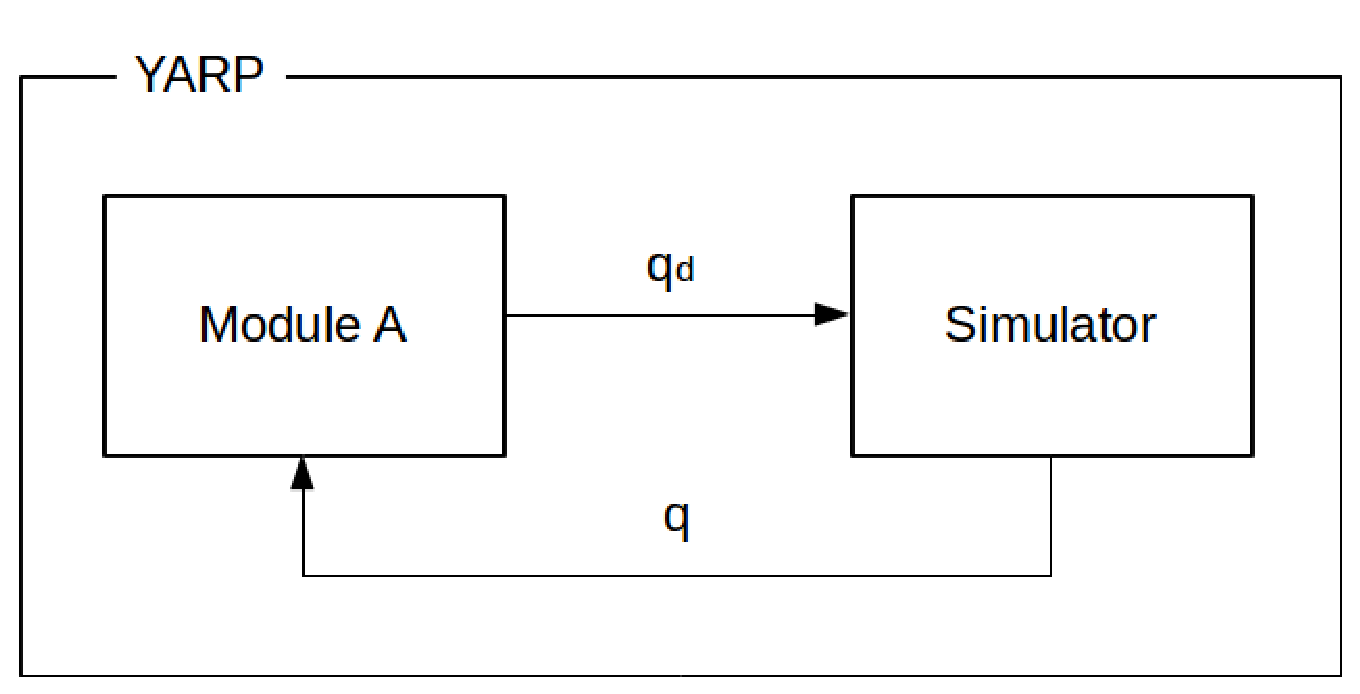
\includegraphics[width=\textwidth]{images/yarp_simulation_a.eps}
                \caption{Module A connected to the simulator}
                \label{yarp_simulation_a}
        \end{subfigure}%
        \\
        \begin{subfigure}[b]{0.45\textwidth}
                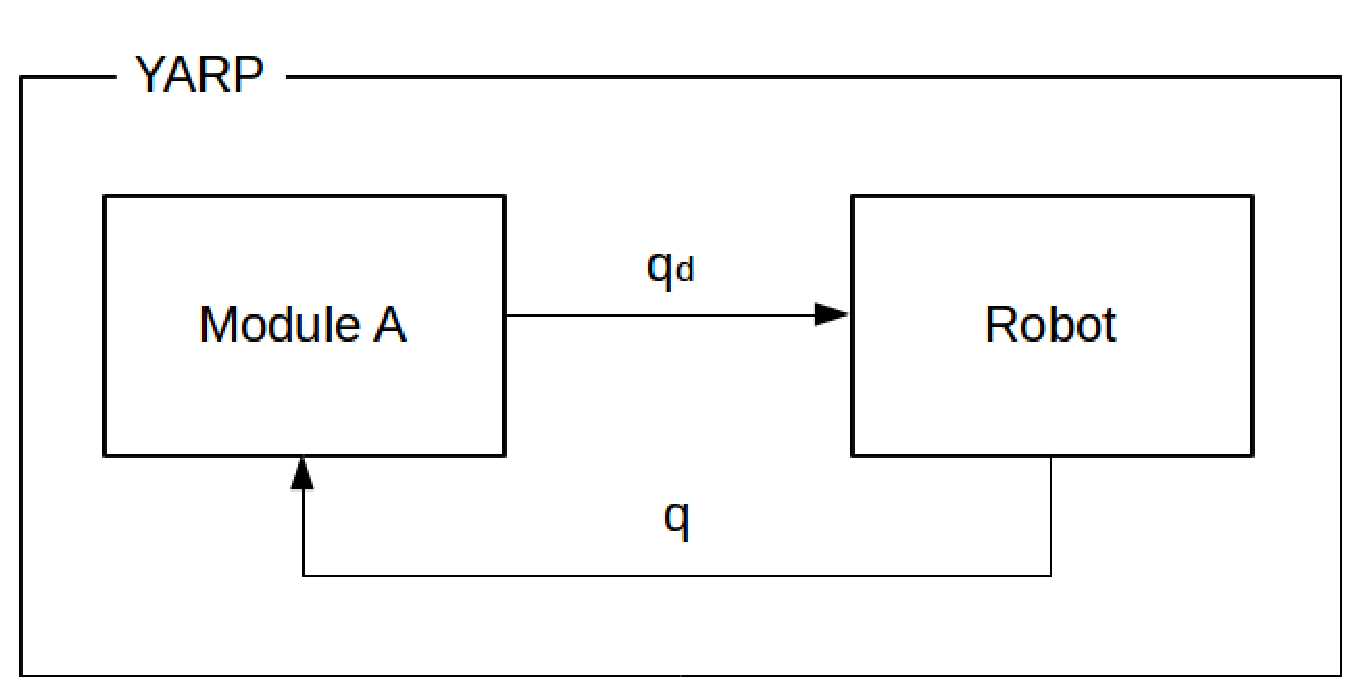
\includegraphics[width=\textwidth]{images/yarp_simulation_b.eps}
                \caption{Module A connected to the robot}
                \label{yarp_simulation_b}
        \end{subfigure}
        \caption{Module A writes desired joint position and read actual joint position without knowing if it is interfaced with the simulator or the robot since they expose the same interface.}\label{yarp_simulation}
\end{figure}

A preliminary stage of simulation during development of both research and production code, has many benefits that increase as the cost of production and maintanance of the hardware increases. Moreso, the ability of seamlessly switching between simulator and robot is an important factor that helps reduce development time and is not prone to errors and artifacts introduced during porting, enabling validation by simulation.
Also the simulator provides fundamental advantages, like the ability to simulate faster than real-time.

\subsection{Related Work}\label{related_work_simulators}
The \emph{Open Dynamics Engine} (ODE, \cite{opende}) is one of the most widely used rigid body dynamics engine in robotics simulation. ODE simulates chains of rigid bodies connected and constrained by different types of joints. It has a built-in collision detection system and implements hard contacts using non-penetration constraint whenever two bodies collide. Beside the large number of project that use it, at the moment the development has been paused. \emph{Bullet} (\cite{bulletpe}) is another dynamic engine. It implements different direct/inverse rigid body dynamic algorithms (eg. Featherstone articulated body algorithm, \cite{Featherstone:2007:RBD:1324846}) as well as different solvers (eg. Mixed Linear Complementarity Problem, MLCP) and contact models. Bullet is used for a wide range of projects and its community is active and continues to improve it constantly.

\emph{OpenRAVE} (\cite{diankovthesis}), \emph{Webots}  (\cite{Michel04cyberboticsltd}), \emph{V-REP} (\cite{conf/iros/RohmerSF13}) and OpenHRP  (\cite{journals/ijrr/KanehiroHK04}) all use the aforementioned dynamics engine, or variations thereof, and differ itself in the offer of libraries that aid in modeling, planning, controlling simulated systems.

The most recent MuJoCo (\cite{conf/iros/TodorovET12}) offers a novel approach to simulating dynamic systems with contact, and performed well comparatively to other simulators in a set of benchmarks\cite{erez15}.

In particular, in the last years, we have been witness to the significant investment in resources to provide reliable simulation tools for humanoid robots~\cite{Hsu14} which has been fostered by the Darpa Robotics Challenge (DRC). The results of this investment has allowed teams to compete virtually before qualifying for expensive robot hardware.  
Gazebo~\cite{koenig2004design} is one of the most popular general-purpose robot simulators, funded through DRC efforts.
It is a generic multi-robot simulator, historically developed taking into account simulations in outdoor environments, and especially interesting nowadays for its high level of integration, as it provides realistic simulation of sensory feedback. including noise modeling. Other than ODE and Bullet, it allows to use DART \cite{DART} and the promising SimBody \cite{Sherman2011241}, which is the only supported engine at the moment implementing variable step integration. For these reasons, and for its complex high level architecture, Gazebo has been used to compare algorithms for navigation and grasping in a controlled environment.
To this day, its development is mainly performed by the Open Source Robotics Foundation (OSRF) under an open-source license, and is supported by a very large community.

Gazebo is expandable by means of its plugin structure: thusly our YARP interface to the Gazebo simulator is a collection of plugins, the \emph{gazebo\_yarp\_plugins}, that offer features wich will be described to various degrees of detail in the current section. 


\subsection{Software Architecture}\label{structure}
Gazebo plugins are C++ classes that extend the functionalities of Gazebo, while YARP device drivers are C++ classes used in YARP for abstracting the functionality of robot devices.
Usually, each class of gazebo\_yarp\_plugins embeds a YARP device driver in a Gazebo plugin. 

{\bf Gazebo Plugins}
A plugin is a piece of code compiled as a shared library and inserted into the simulator. A plugin has direct access to all the functionalities of Gazebo from the physics engine to the simulated world. There are 4 types of plugins in Gazebo: \textbf{world}, \textbf{model} and \textbf{sensor} plugins are attached to and control a specific simulated world/model/sensor respectively, while \textbf{system} plugin are specified on the command line and loads during the Gazebo startup.


{\bf YARP \emph{Device Drivers}}
YARP provides special devices that act as network proxies and make interfaces available through a network connection. This allows accessing devices remotely across the network without code change.

A device driver is a class that implements one or more interfaces. There are three separate concerns related to devices in YARP:
\begin{itemize}
\item Implementing specific drivers for particular devices
\item Defining interfaces for device families
\item Implementing network wrappers for interfaces
\end{itemize}
For example the Control Board device driver implements a set of interfaces that are used to control the robot (IPositionControl, ITorqueControl, etc.) and another set of interfaces to read data from the motors (IEncoders, etc).

\subsubsection{Gazebo-YARP Plugins}
The gazebo\_yarp\_plugins is composed of:
\begin{itemize}
    \item Gazebo plugins that instantiate YARP device drivers,
    \item YARP device drivers that wrap Gazebo functionalities inside the YARP device interfaces.
\end{itemize}
The plugins/devices implemented are the \emph{Control Board}, \emph{6-axis Force Torque sensor}, \emph{Inertial Measurement Unit} (IMU) and a \emph{Clock} plugin used for synchronization. The plugins stream data which is generated by the Gazebo simulator, and thus support all the features of the simulator, such as modelling Gaussian noise on the IMU readings.
While the first three plugins are directly related to the simulated objects and sensors, the last one is a system plugin that synchronizes the YARP modules with the simulation time.

\begin{figure}
        \centering
        \begin{subfigure}[b]{0.475\textwidth}
                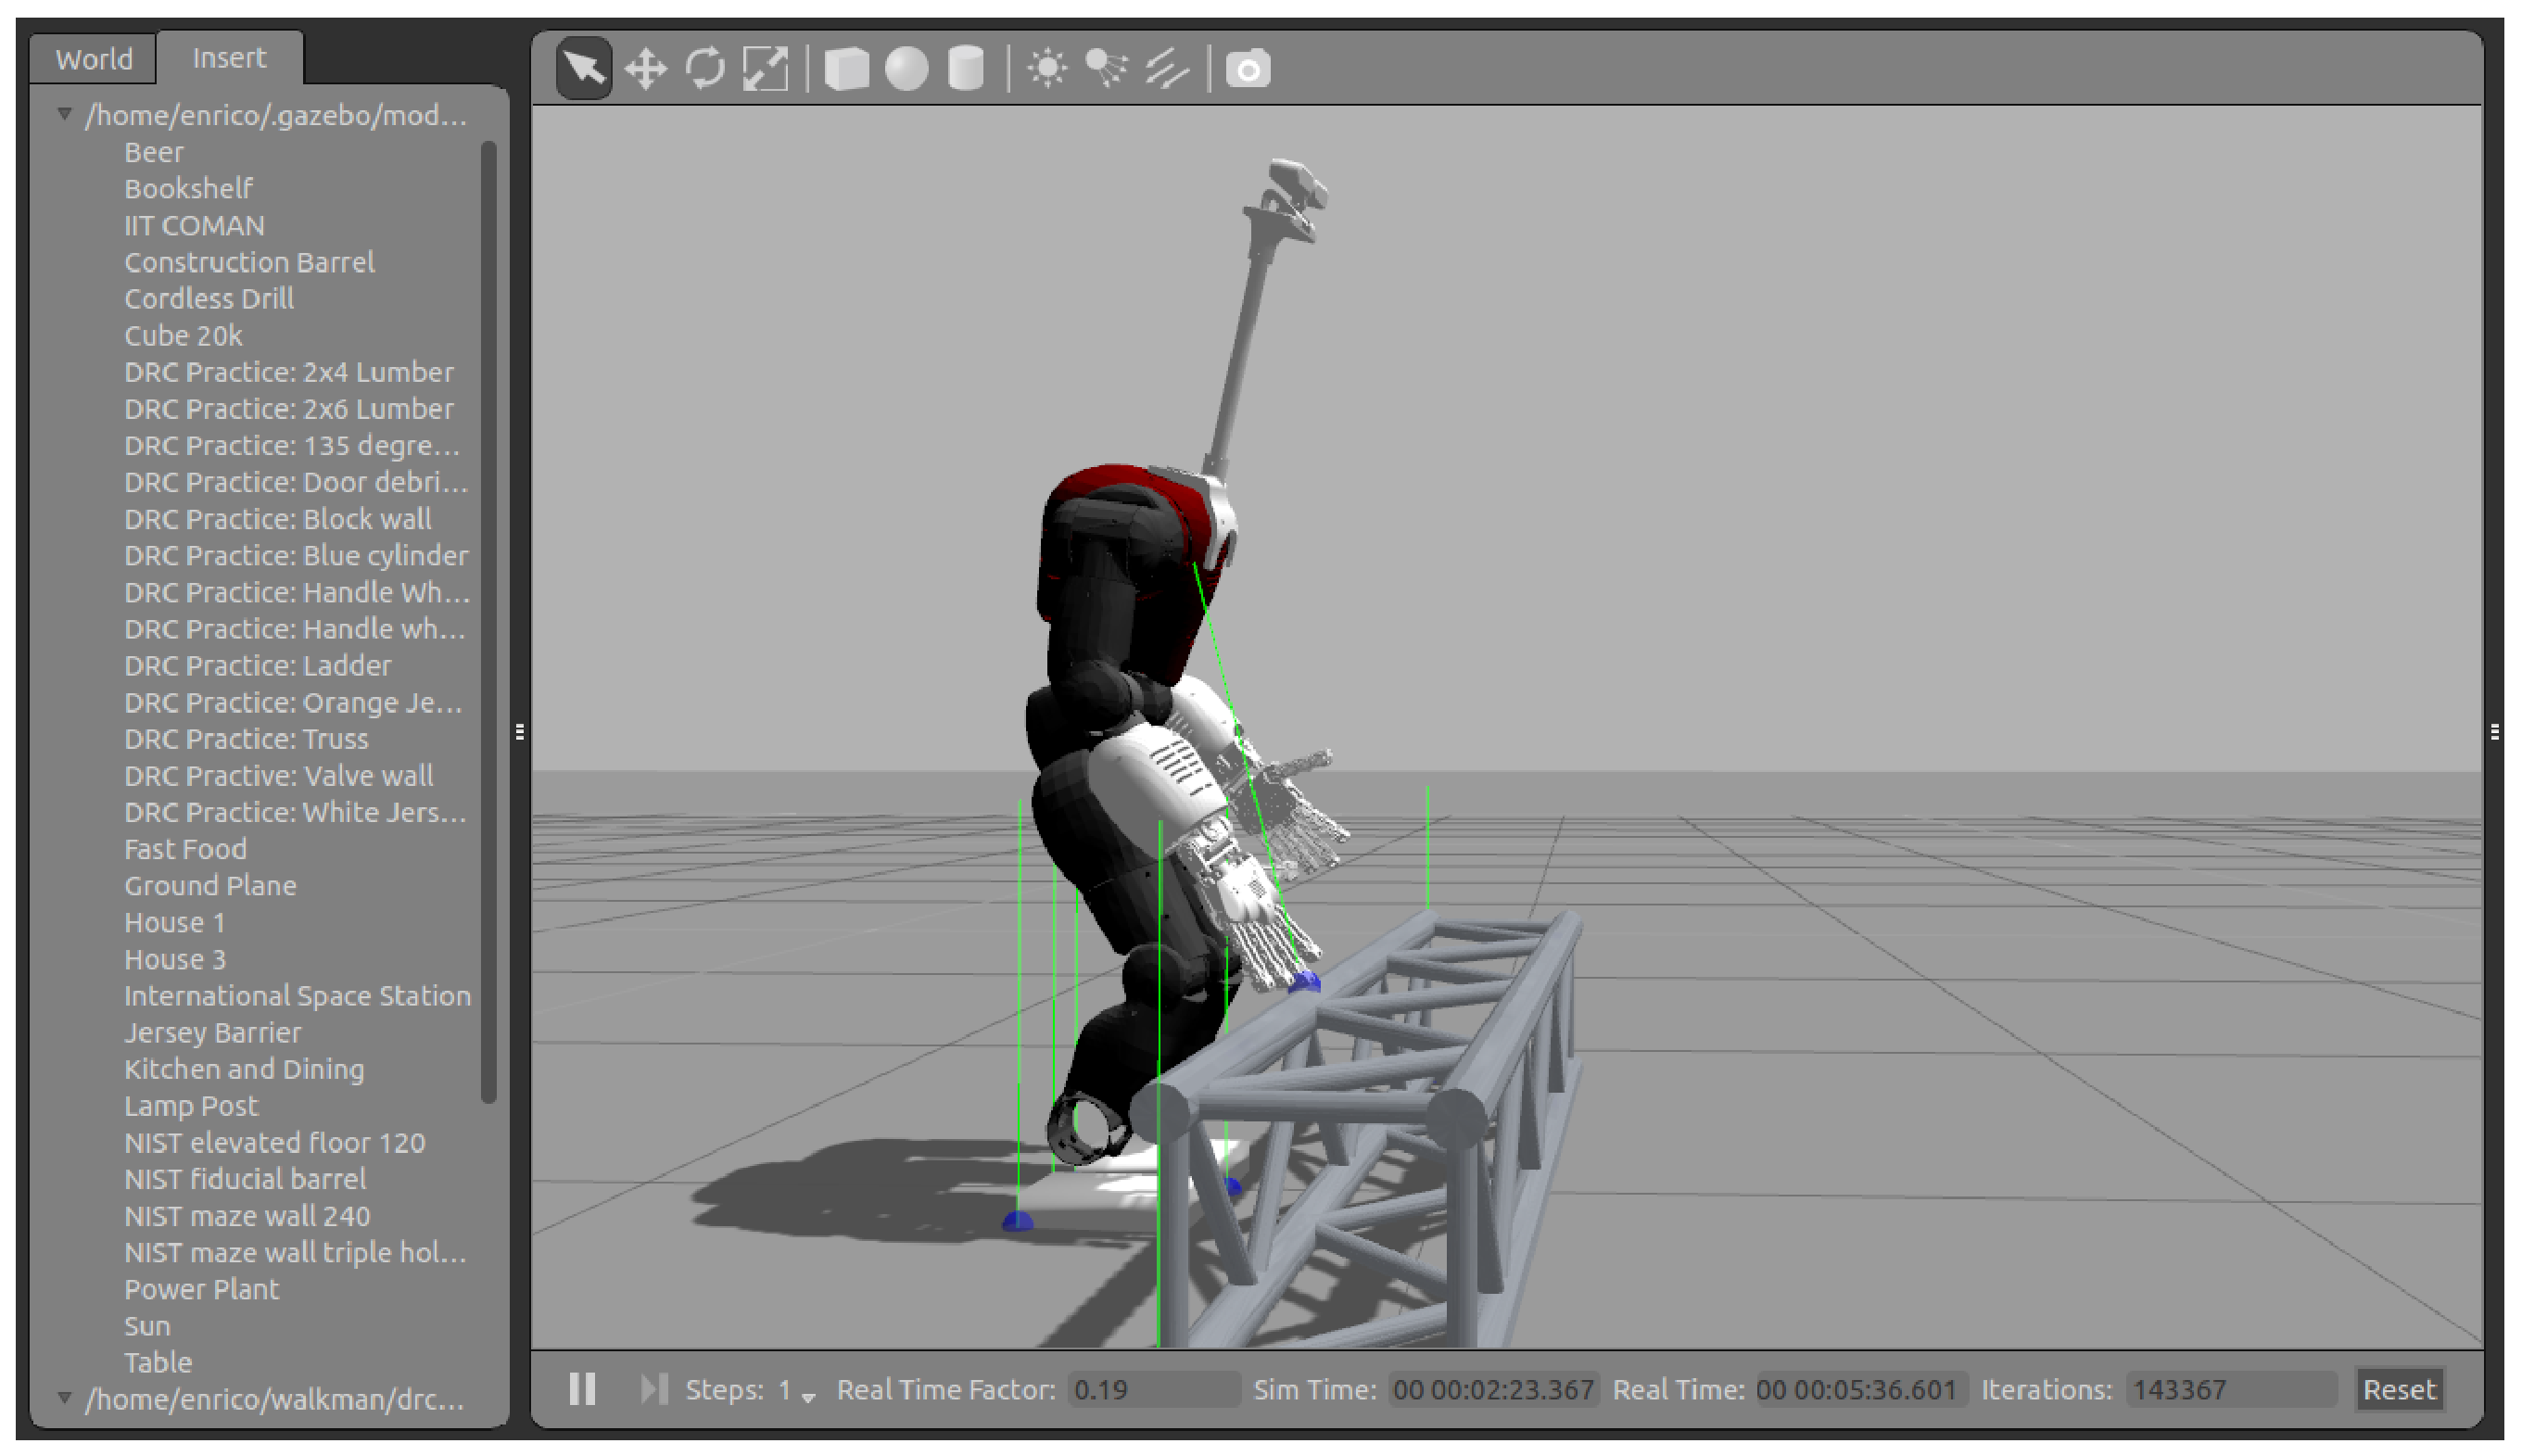
\includegraphics[width=\textwidth]{images/coman_ft_a.eps}
                \caption{Gazebo interface with COMAN}
                \label{yarp_simulation_coman_a}
        \end{subfigure}%
        \\
        \begin{subfigure}[b]{0.475\textwidth}
                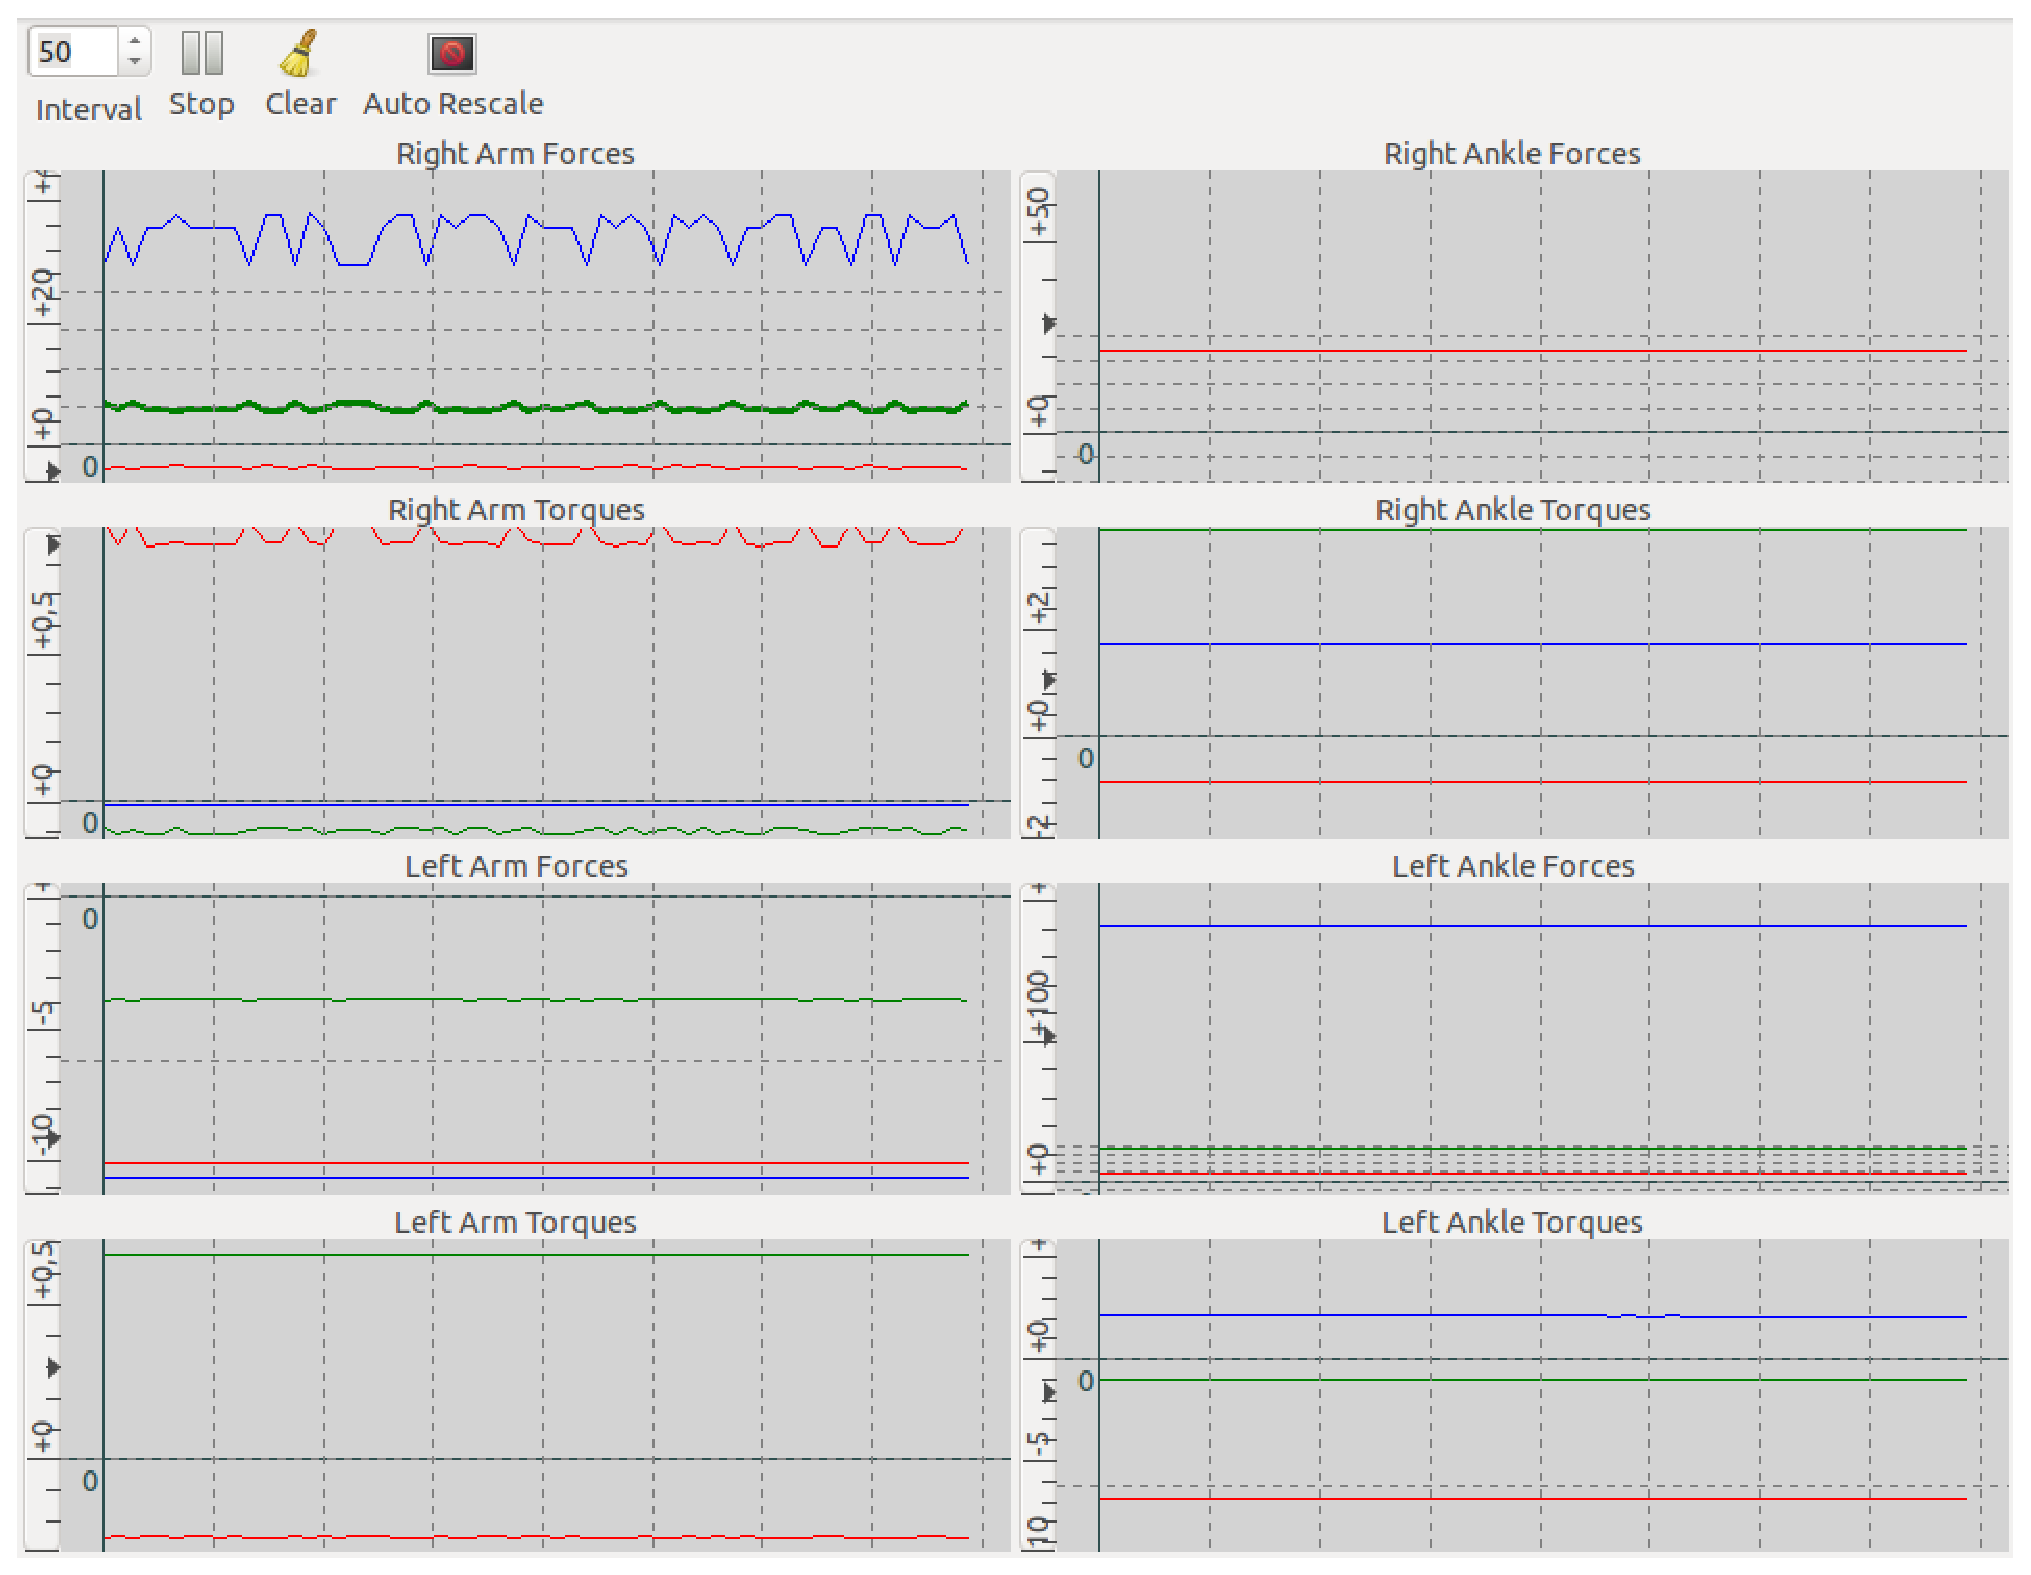
\includegraphics[width=\textwidth]{images/coman_ft_b.eps}
                \caption{A yarpscope showing on-line the forces and the torques at each Force/Torque sensor}
                \label{yarp_simulation_coman_b}
        \end{subfigure}
        \\
        \begin{subfigure}[b]{0.475\textwidth}
                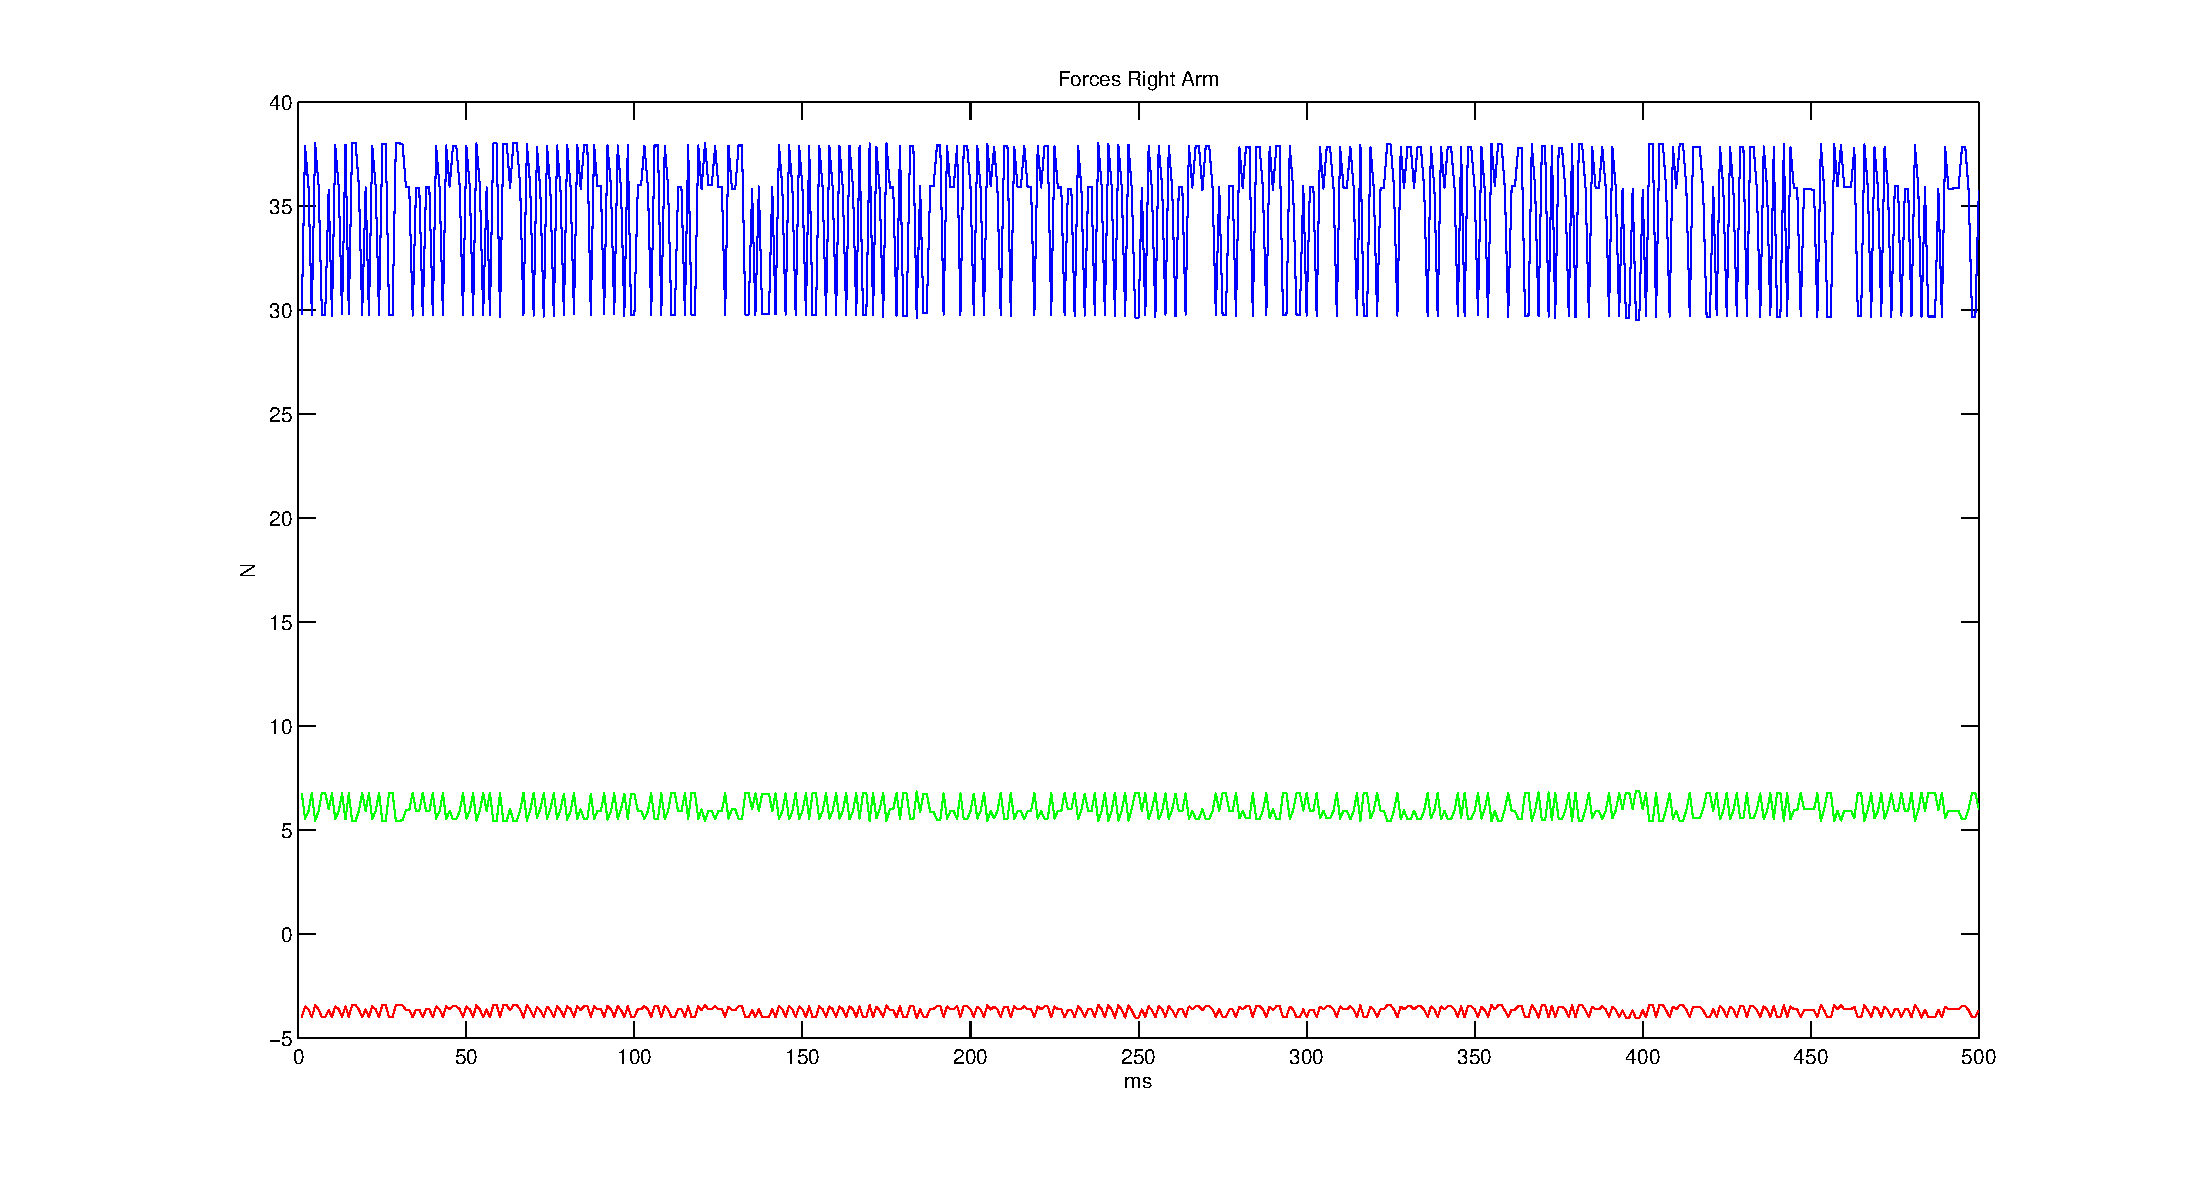
\includegraphics[width=\textwidth]{images/coman_ft_c.eps}
                \caption{Plot of forces measured at the simulated Force/Torque sensor placed on the right arm. Forces along x,y and z are respectively in red, green and blue}
                \label{yarp_simulation_coman_c}
        \end{subfigure}
        \\
        \begin{subfigure}[b]{0.475\textwidth}
                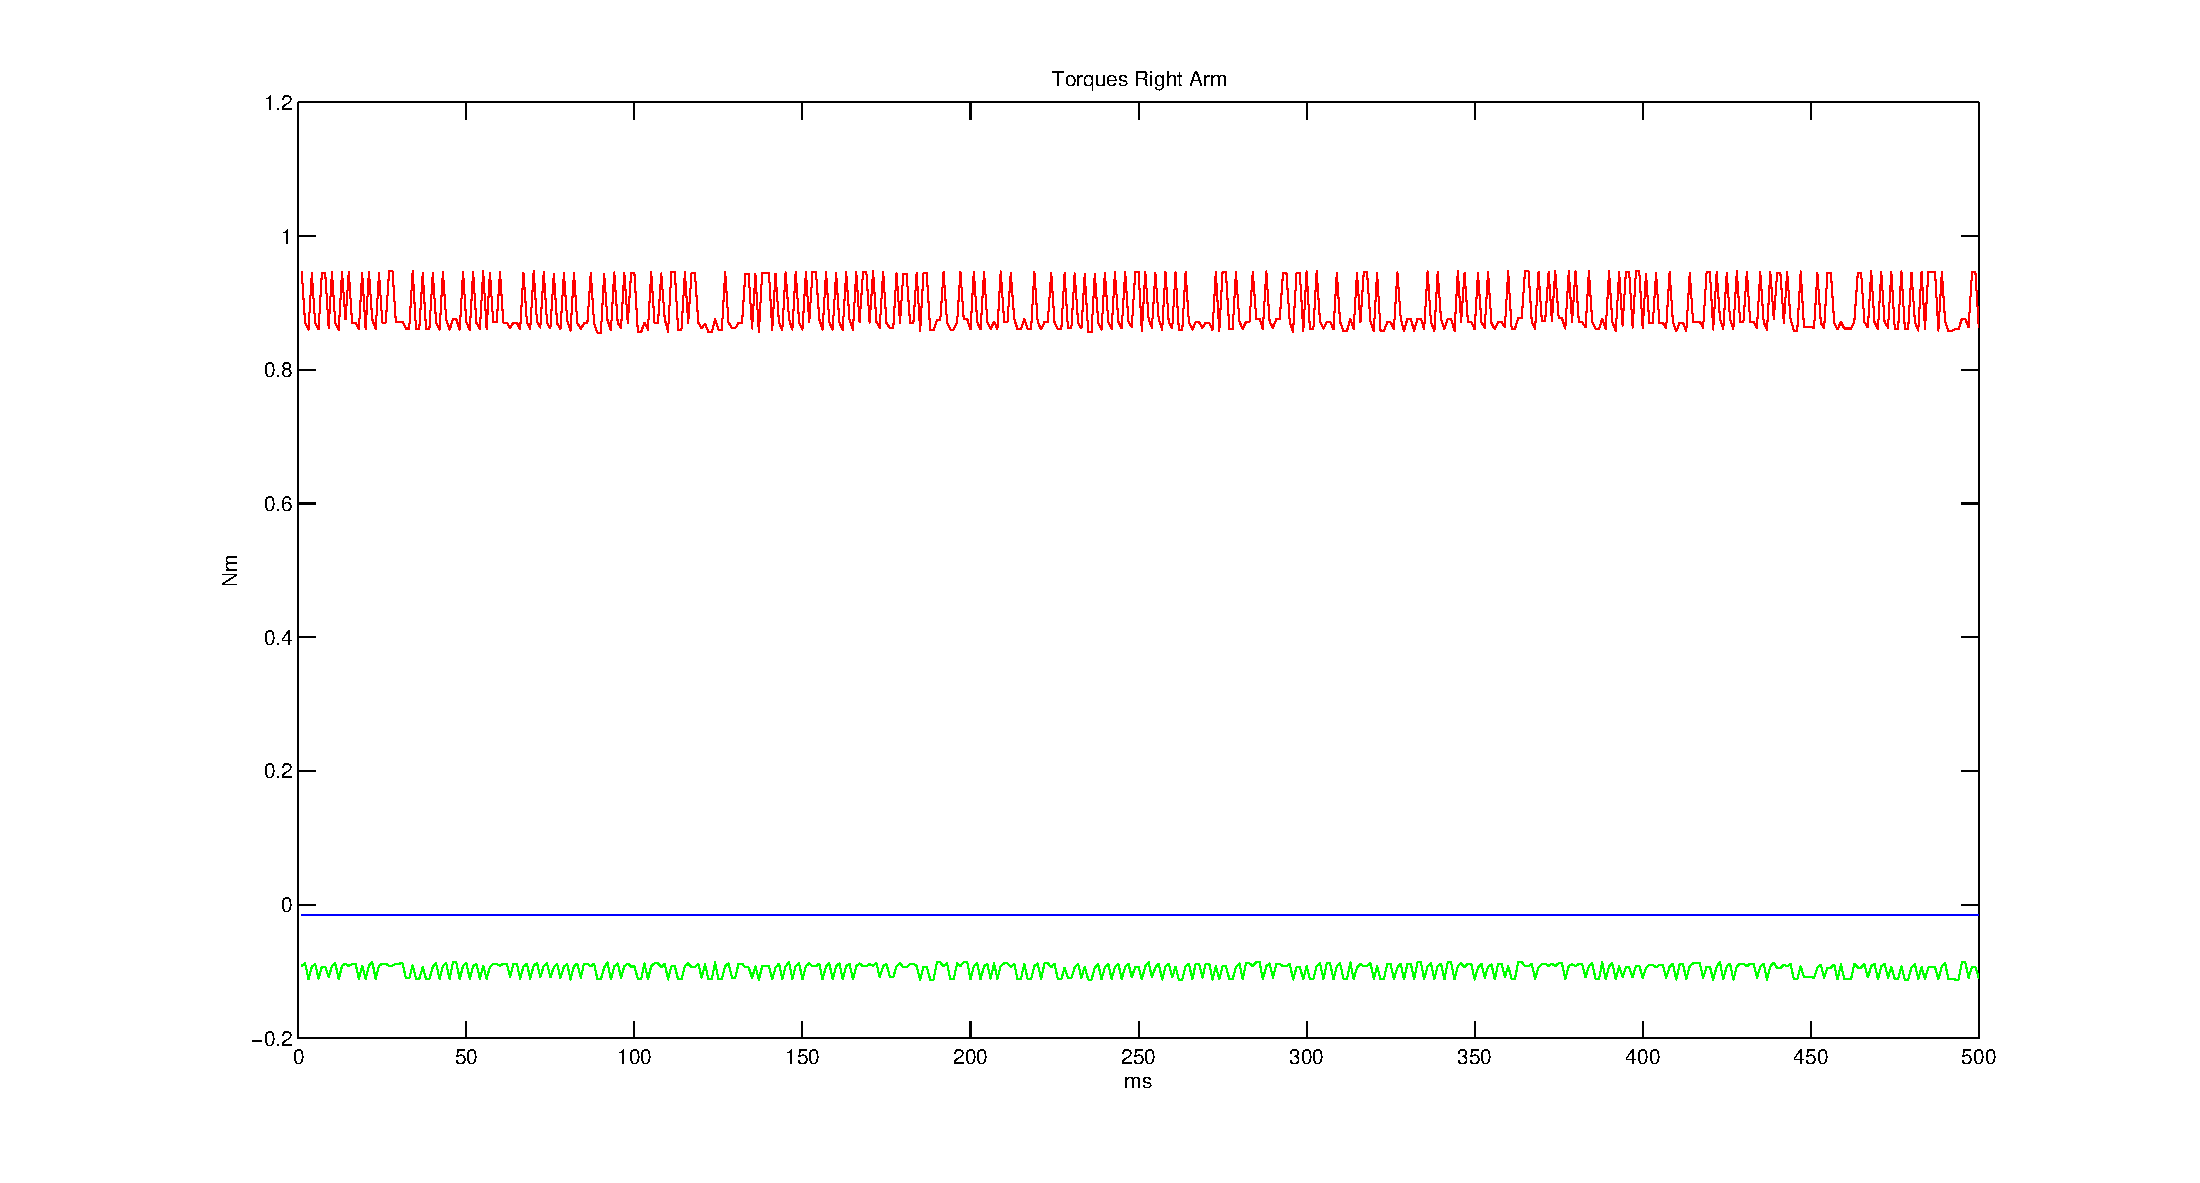
\includegraphics[width=\textwidth]{images/coman_ft_d.eps}
                \caption{Plot of torques measured at the simulated Force/Torque sensor placed on the right arm. Torques along x,y and z are respectively in red, green and blue}
                \label{yarp_simulation_coman_d}
        \end{subfigure}
        \caption{A Gazebo simulation running COMAN interacting with debris}\label{force_torque}
\end{figure}

\subsubsection{Control Board}
The Control Board plugin allows to control the robot using YARP Interfaces, it is implemented as a Gazebo Model plugin. Every control board allows the user to control one or more joints (a kinematic chain such as the arm or leg, etc.) as specified in a configuration file. For each controlled joint the control board opens different interfaces, permitting the use of different type of controllers for each joint. Such interfaces include position control, torque control, encoders reading, torque measurement and joint impedance control. Usually the number of instantiated control boards is equal to the number of kinematic chains.
This duality between control boards and kinematic chains can be abandoned for the sake of performance on the real hardware, since every control board is usually implemented by a thread that streams data in a specified port. In that case, typical whole-body control then has to collate the network data coming from each control board and infer the global state of the robot. Each control board, during every cycle of simulation, reads position, velocity and torque values from the simulated joints and sends desired joints position or torques to the simulator. The values read from the simulator are broadcasted through YARP interfaces in the YARP network, in a similar way the desired joint values come from YARP interfaces (Figure \ref{control_board}). The following YARP interfaces are used to control the robot.
\begin{itemize}
\item \textbf{IPositionControl}: a position control with a linear trajectory generator considering a max joint speed
\item \textbf{IPositionDirect}: a position control using Gazebo position PIDs
\item \textbf{ITorqueControl}: a perfect torque follower
\item \textbf{IImpedanceControl}: a joint impedance control with the following law
\begin{equation}
    \tau_d = -P_d(q-q_d) - D_d\dot{q} + \tau_{offset}
\end{equation}
where $q_d$ is the desired equilibrium position, $P_d$ is the desired joint stiffness and $D_d$ is the desired joint damping. $\tau_{offset}$ is an extra term that can be used for gravity compensation or inverse dynamics control.
\end{itemize}
Furthermore, the Control Board implements the \textbf{IControlMode} interface that allows to change the type of controller online. All these interfaces are also available on the robot and they have the same behaviour.

\begin{figure}[h!]
  \centering
    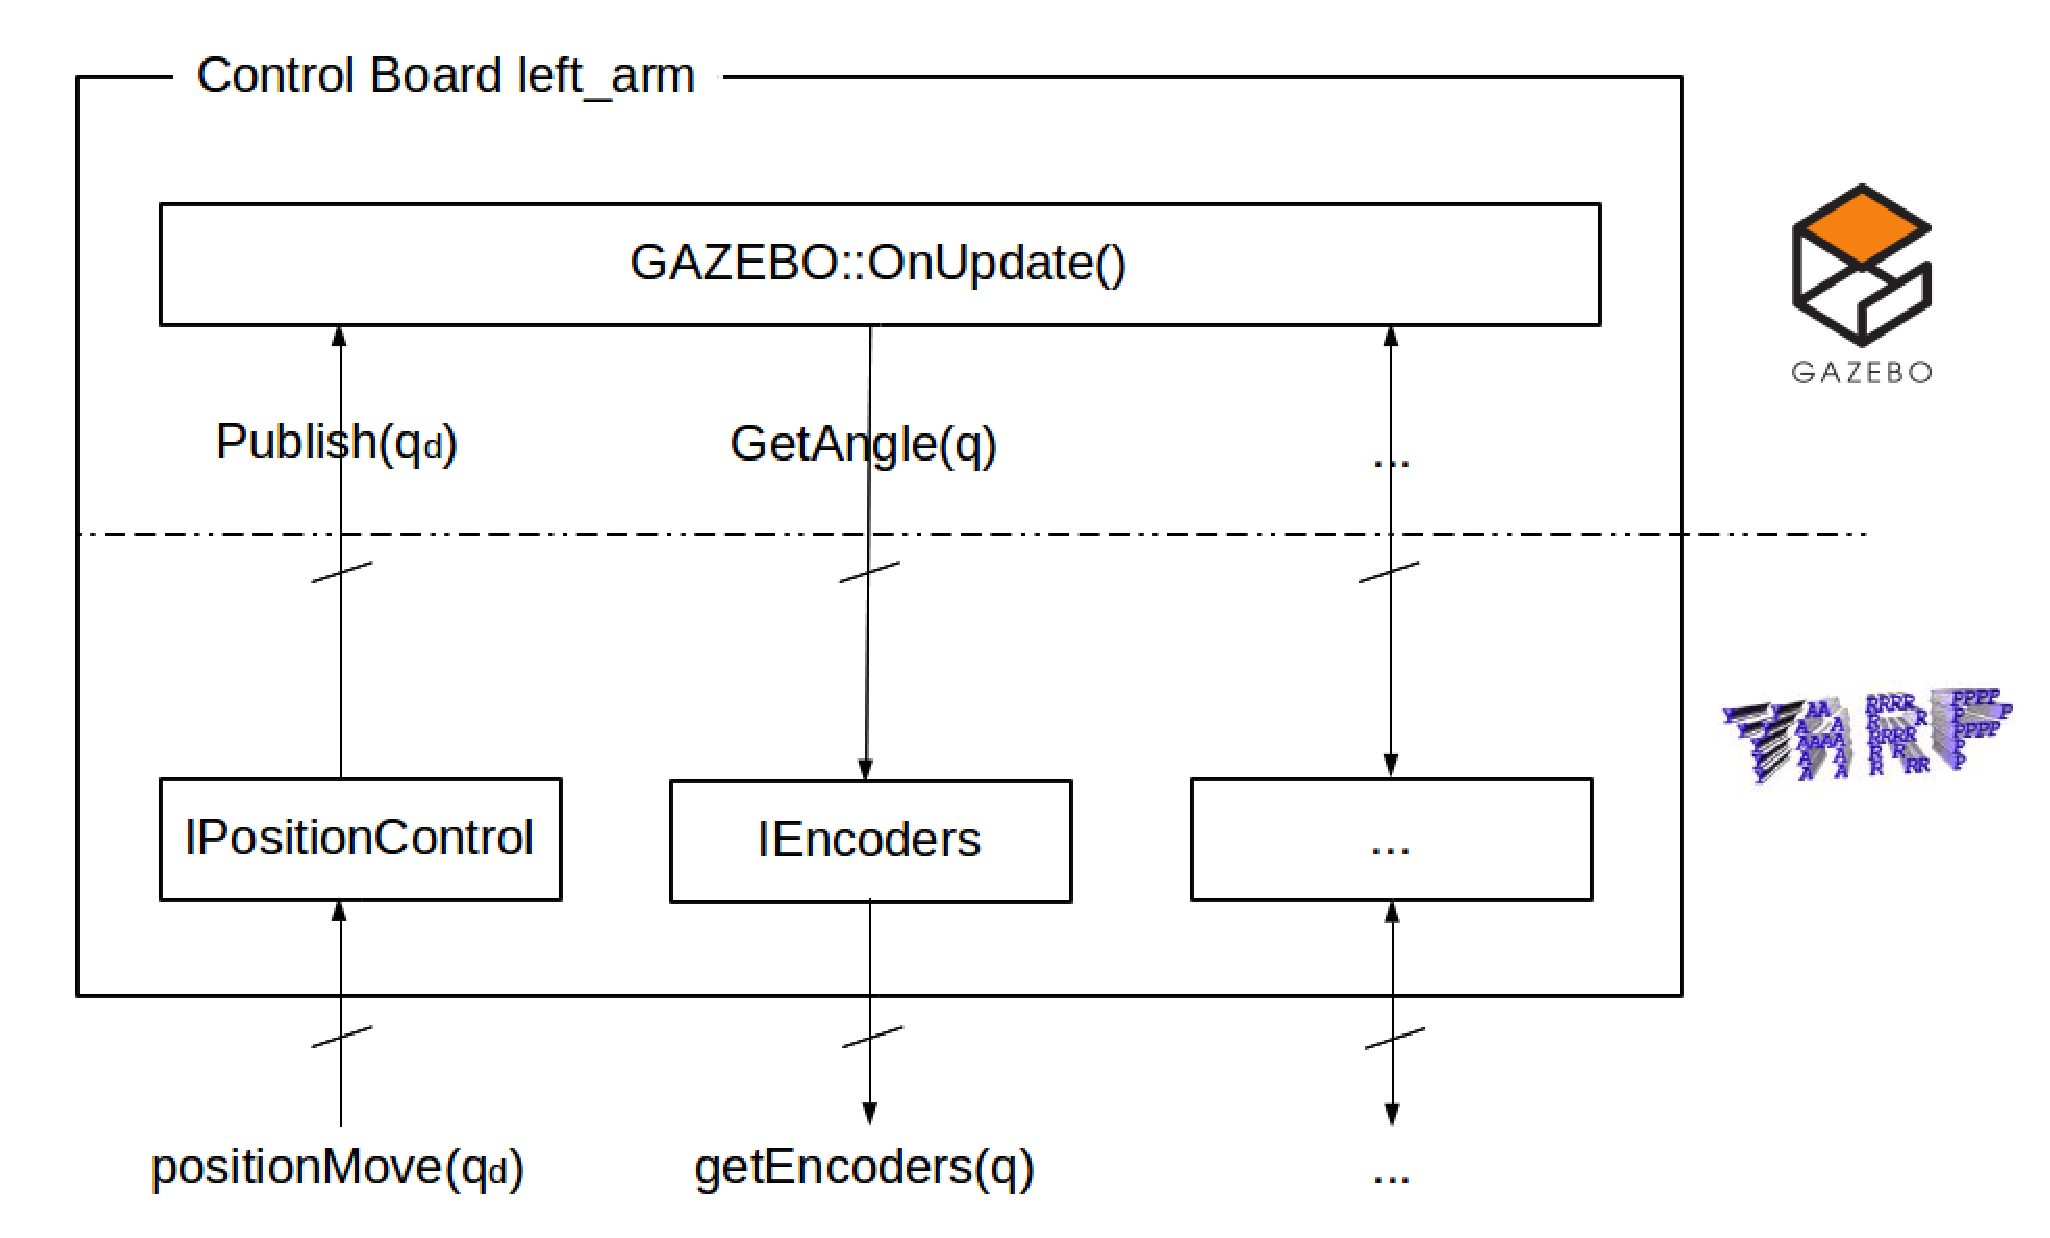
\includegraphics[width=0.5\textwidth]{images/control_board.eps}
    \caption{Control Board plugin for the left\_arm kinematic chain. yarp::IPositionControl interface has a method positionMove() that can be used to set joint values inside a YARP module. The plugin implements such interface by calling the Publish() method inside the Gazebo API to move the simulated joints at each OnUpdate().}\label{control_board}
\end{figure}

\subsubsection{6-axis Force/Torque sensor}
A Force/Torque sensor measures a wrench in the robot structure (Figure \ref{force_torque}). The sensor streams the data that are provided by Gazebo from a joint information. In fact, simulators like ODE use a maximal coordinate system, meaning that every body is simulated as an unconstraied ribid body (6DOFs), where constraints are enforced through the LCP formulation. This makes so that also joints are constraints, and since during simulation tipically the solver allows for constraint violation to a certain degree, which is proportional to the forces acting on the system and the equivalent stiffness of the constraint, such violation can be used to infer the forces and torques acting on the joint. \todo{add more details about the stiffness of joints} On the YARP side, the reading of a generic sensor is implemented as a \textbf{IAnalogSensor} interface (Figure \ref{ianalog_force_torque}). The broadcasted data is a vector of six numbers representing the forces and the torques applied on that reference frame.

\begin{figure}[h!]
  \centering
    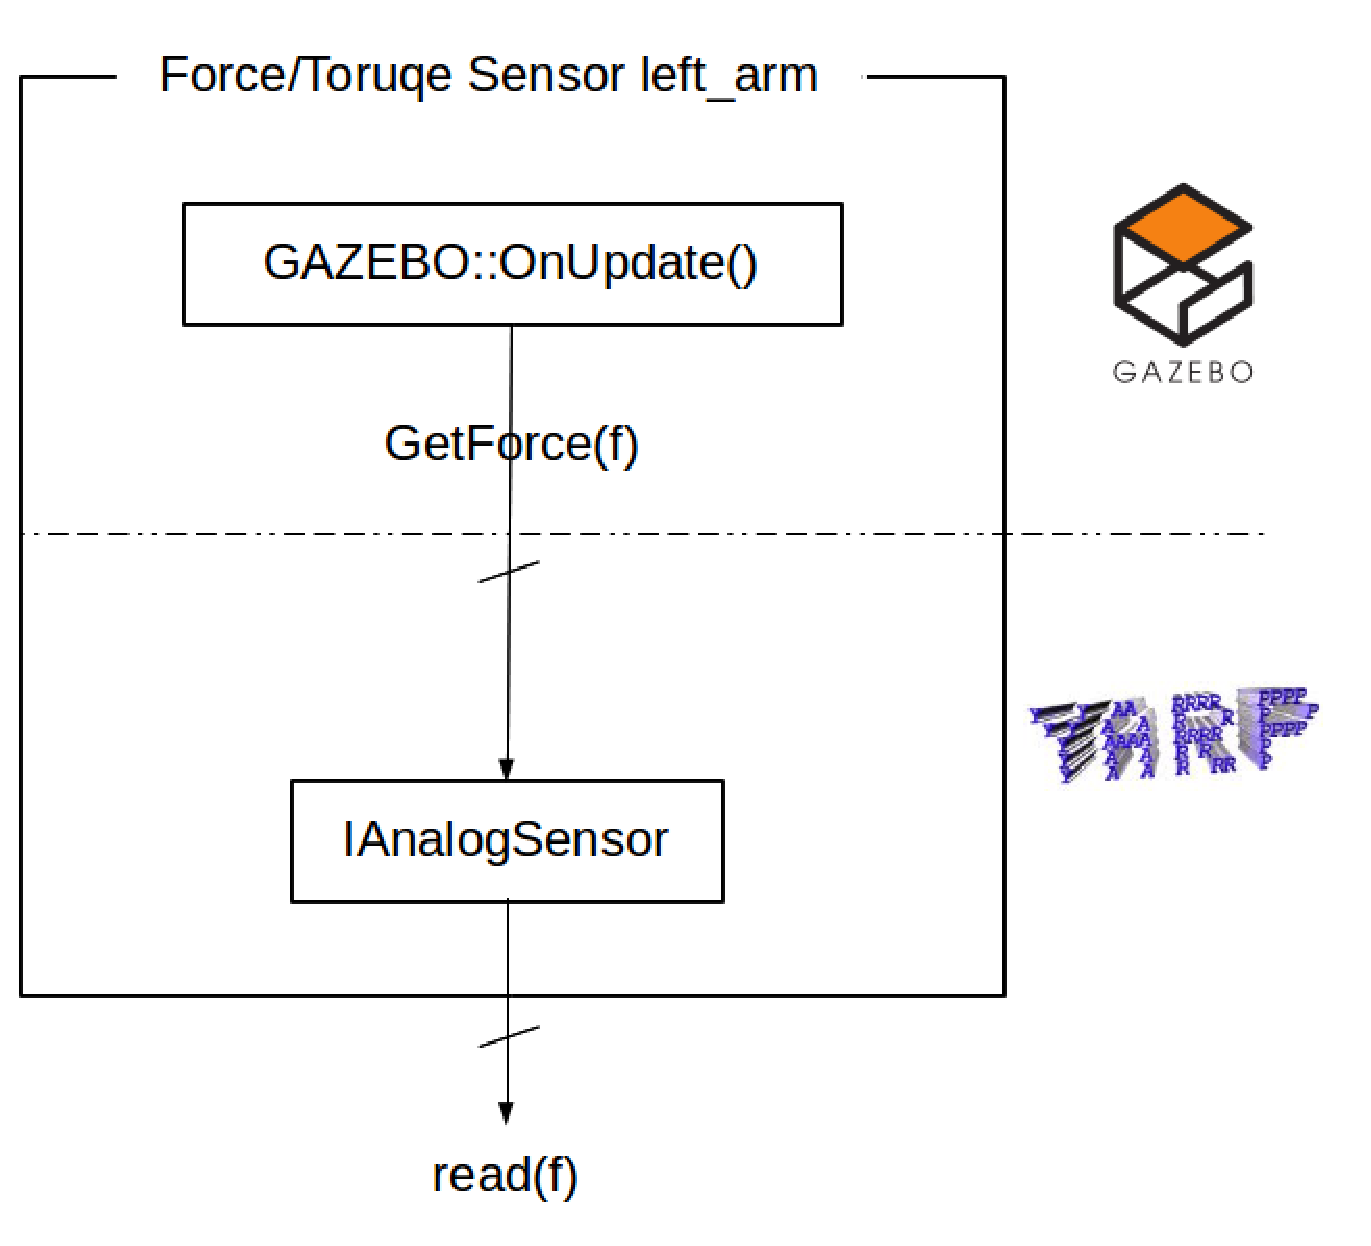
\includegraphics[width=0.475\textwidth]{images/ianalog_force_torque.eps}
    \caption{The Force/Torque sensor in the left arm is implemented as a YARP IAnalogSensor interface. At every step the internal state of the plugin is updated with the last readings of forces and torques from the simulation.}\label{ianalog_force_torque}
\end{figure}

\subsection{Real-Time Simulation of Robotic Systems: Clock}
\begin{figure}
  \centering
    \hspace*{-0.25in}
    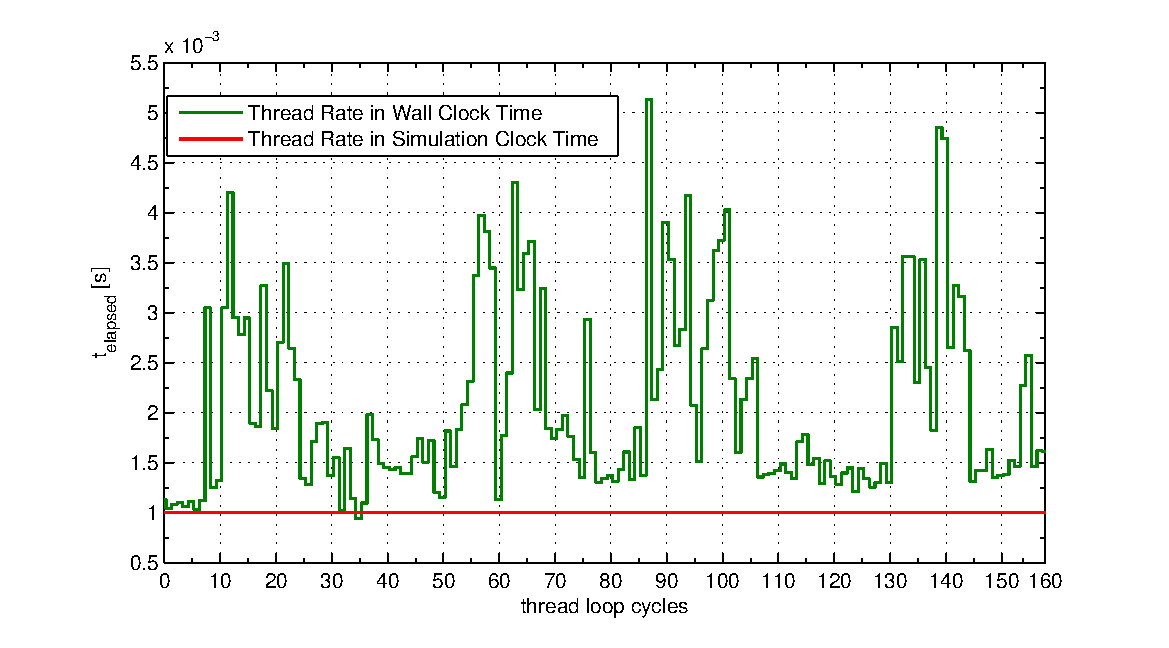
\includegraphics[width=0.51\textwidth]{images/yarp_clock.eps}
    \caption{Time elapsed between each execution of the control loop, measured in simulation clock time and in wall clock time. Desired thread rate is $1$kHz and simulation time step is $1$ms}\label{yarp_clock_real_vs_simulated}
\end{figure}
A fundamental aspect of simulation is the synchronization between the simulation code and the high level task code. Often, ad-hoc solutions emply a simulator-in-the-loop approach were after a certain number of simulation steps, and possibly each step, a control step is executed. In this case, we have true bidirectional synchronization between the simulation and the task code, that is, locked-step simulation. Since our code needs to be indipendent and agnostic of the simulator, it needs to be a networked application, and a synchronization mechanism needs to be put in place. In particular, the low level control algorithms specified in \ref{control_board} is automatically synchronized with the simulation, and mimics the real-time characteristics of the low-level decentralized control running on the joint's boards of a robot. In order to simulate also real-time execution of the high-level code, synchronization between YARP modules and the simulated robot is needed.
A YARP module is a process in which one or more threads are started. When such modules are used in the real robot, the thread rate is timed by the machine (system) clock, also called the \emph{wall clock}. In the same way, the client code's loop needs to be synchronized to the simulated clock when controlling a simulated robot.
The \emph{real-time factor} (\emph{RTF}) of the simulation is given by 
\begin{equation}
    RTF = update\_frequency \times step\_time
\end{equation}
and is kept to one when the desired update frequency is the inverse of the time increased at each step in the simulation.
%because if the real time factor of the simulation is above 1.0 the control could run in general faster than the simulation and this is not realistic. 
For instance if the simulation runs with a real time factor of 0.1, 10 seconds are needed to simulate $1$ second of the physical system evolution. Within this situation, the controller process should also be slowed down 10 times to be coherent with the simulation. To solve this issue a \emph{clock} plugin has been designed that synchronizes the high level control modules with the simulated time when controlling a simulated robot. The idea is similar to the ROS clock plugin for the Gazebo simulator, in that it is not a lock-step synchronization, meaning that in order to run the simulation faster than real-time we need the control code to be fast enough, since the control code will be synchronized with the simulation clock but the simulation will not wait for the control code to complete execution before starting the next simulation step.

The \emph{clock} plugin is implemented as a System plugin and publishes on a YARP port the time information from the simulator. For every simulation step, the simulation time is incremented and the timestamp is sent via socket. The data sent via this port acts as signal for a $1$Khz simulated scheduler that wakes up the control threads that need to be woken up.

In general, all the YARP functions that provide access to the computer internal clock and support thread scheduling can be synchronized with an external clockof choice, be either coming from the simulator or other means (this is enabled with the \emph{YARP\_CLOCK} environment variable). Classes supporting periodic threads (\emph{RFModule} and \emph{RateThread}) are therefore automatically synchronized with the clock provided by the simulator. The \emph{yarp::os::Time} functionalities are also transparently working using the wall-clock or the simulation clock depending on the environment variable. Thread sleeps are performed using the wall or simulated time depending on the circumstance.

More in detail, when synchronized with the simulation clock the \emph{yarp::os::Time} delay does not explicitly sleep on a wall clock, rather a scheduler is synchronized with the simulation clock by performing blocking reads on the \emph{YARP\_CLOCK} port. This scheduler wakes up the threads that required a delay just once, when they have slept for the desired duration. Compared to the ROS::Time implementation which uses small sleeps on wall clock to check synchronization with the simulated clock, this allows to run simulations both slower and faster than real time and still have synchronization between threads and controls. In any case, when accessing the simulated clock Experiments showed the approach to be successful in synchronizing $1$kHz control loops against simulations running $1$kHz, thus having a $1$ms clock granularity.

A similar solution for synchronization has been consequently used also in \cite{wbi14}.

\subsection{Notes on Simulation of compliant, highly redundant robots}
The problem of simulating compliant humanoid robots in particular, and highly redundant robots in general, is the computation burden due to the large amount of joints (and thus, rigit bodies) that need to be simulated.
Work is ongoing to properly simulate these systems on Gazebo, by using the Spong model and effectively doubling the number of simulated joints.\todo{input Spong Equation} While this approach allows to accurately simulate robot compliance but poses performance problems.
A practical approach that has been used for the simulation of the robots developed at the Istituto Italiano di Tecnologia that are equipped with SEA joints, in particular when used in position control schemes, has been to tune the system PIDs to the actual joint compliance in the robot. Assuming a perfect controller on the physical robot, and taking into account that the simulated PID has a torque feedback, then the P gain is dimensionally a stiffness, and the D gain is a damping.
Technically, simulating compliant robots is easier than simulating stiff systems, were implicit integration schemes are needed for stability. \todo{cite ref}
The current Gazebo simulator uses a semi-implicit integration scheme, nonetheless simualaing very rigid robots (through very rigid PIDs) requires small integration steps, which compromise simulation speed. In our experiments, simulation is always run with a $1$ms timestep.

\subsection{Conclusions}
In this section we have presented a set of Gazebo plugins, named \emph{gazebo\_yarp\_plugins}, that allow to connect the robotics framework YARP to multi-purpose simulator Gazebo. Gazebo was chosen since it is easy to use, it has the possibility to switch between different rigid multi-body dynamics engines, it is Open-Source and has an active community. Our plugins are based on YARP device drivers in order to have the same interfaces in the real and simulated robot. This allows to write modules that will work both in the simulator and in the real robot without the need to modifiy the code. This is a very important paradigm in robotics since it minimizes the chance of introducing errors due to porting of the code, and allows for automatic validation by means of simulation. Furthermore the simulator becomes a tool that helps the developer in testing and validating before using the real platform.
Such plugins consist in: a Control Board plugin to control the robot, a Force Torque sensor plugin and an IMU plugin. A special plugin dedicated to synchronization between modules and simulator was also implemented. The plugins were tested to simulate several humanoid bipedal robots, including the COMAN, iCub, and WALKMAN from the Istituto Italiano di Tecnologia.


%%%%%%%%%%%%%%%%%%%%%%%%%%%%%%%%%%%%%%%%%%%%%%%%%%%%%%%%%%%%%%%%%%%%%%%%%%%%%%%%
\section{Simulating Grasps}

Despite increasing popularity of compliant and underactuated hands, there exist few analytical and simulation tools for modeling such hardware.  High-fidelity predictive tools are important in mechanism design as well as grasp planning and optimization to exploit the favorable features of compliant hands.

The following section will report studies \cite{Rocchi2016-jq} on a variety of simulation techniques to predict the success of a compliant gripper on irregular objects.  In particular, performances of a new simulator will be presented, that integrates compliance simulation with a recent Boundary Layer Expanded Mesh (BLEM) technique for enhancing stability of contact normal and penetration depth estimation.
The novel simulator is compared against existing ones using a set of stability and fidelity indices: \emph{contact force smoothness} and \emph{contact position and normal stability}.
Scores along these indices are correlated with the simulator's accuracy of predicting the success/failure of a given grasp pose and preshape.  
A testing set of 13 grasps of varying success rate on physical hands were manually generated for the  \emph{RightHand Robotics} \emph{Reflex Hand} and \emph{Pisa-IIT} \emph{Soft Hand} on $4$ objects with a known 3D model and mass distribution. 
Each grasp is simulated using multiple techniques, and experiments find that the novel simulator leads to improvements both in the stability indices, predictability of grasp success, and reduction of simulation artifacts.

The critical point of the evaluation lies on defining appropriate metrics, which can be considered universal in assessing the capabilities of a grap simulator to predit the behavior of compliant grippers grasping rigid objects. The physical and simulated experiments also have been designed to both highlight the importance of contact stability and accuracy during grasping (e.g. picking grasp poses where object ridges and geometric qualities of the object influennced the grasp outcome), and the importance of correctly simulating compliance (e.g. scenarios where the objec lies on the table and the hand fingers need to slide on the surface to perform a cage grasp).
%is susceptible to contact stability, that the \emph{BLEM + hierarchical clustering} provides the best indices over the set of techniques presented, and illustrate some examples where a physical grasp grading can give unique insights over the stability of grasps empowered by environmental constraints, grasps of kinematic chains, and grasps of objects where the mass distribution is known.

\subsection{Stable Simulation of Underactuated and Compliant Hands}
%%%%%%%%%%%%%%%%%%%%%%%%%%%%%%%%%%%%%%%%%%%%%%%%%%%%%%%%%%%%%%%%%%%%%%%%%%%%%%%%
\begin{figure}[!hbt]
\begin{center}
        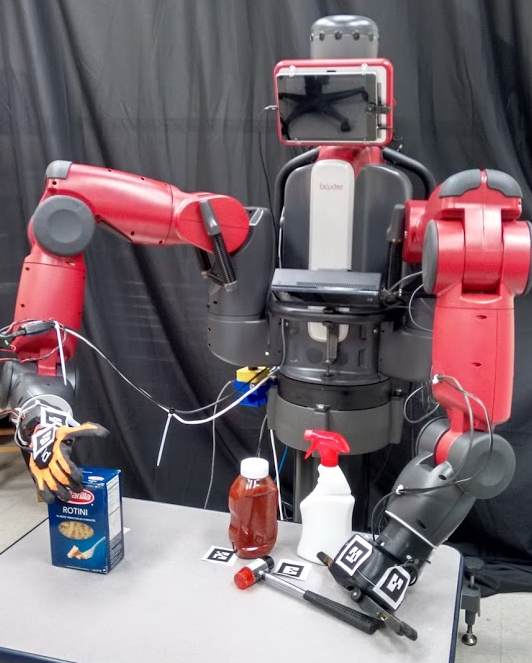
\includegraphics[width=0.75\columnwidth]     {images/ssoch/baxter_HDR}
        \caption{the Baxter robot equipped with a Reflex Hand and a Soft Hand with the gasp set used for the experiments}
        \label{fig:baxter}
        \end{center}
\end{figure}
%[KH: Irrelevant]
%In recent years, the variety and complexity of robotic hardware has been influenced by the steady rise of rapid prototyping tools, and started to move from lab-spaces to real environments while requiring designs to be cheaper and more robust.
An increasing number of robot hand designers have been moving towards devices that make use of compliance and underactuation. The iHY~\cite{Odhner14}, Reflex Hand~\cite{ReflexHand}, Pisa/IIT SoftHand~\cite{Catalano14}, Robotiq 3 fingers gripper~\cite{Robotiq3Finger}, RBO~\cite{Deimel13} and RBO2~\cite{Deimel14} and Yale Hands~\cite{Ma13} are recent examples of underactuated compliant hands. The main benefits of such designs include hardware robustness and the capability of adapting the hand shape to a wide range of grasped objects. Underactuated hands provide many degrees of freedom of movement (DoFs) while being actuated by just a few degrees of actuation (DoAs), and clever passive mechanisms are designed to coordinate the actuation of multiple DoFs, which simplifies the otherwise complex hand control problem. %[KH: "taming" is too dramatic] taming the complexity of the hand control problem by means of intelligent hardware design.
Although compliant hands are built to be more robust to sensing uncertainties than rigid ones, they typically increase actuation uncertainties. As a result, successful grasping still requires deliberation, particularly for objects of irregular shape or mass distribution. It is also challenging to grasp objects in clutter because fingers may be disturbed by inadvertent contact with the environment or other objects. Hence, model-based predictions of motions and forces can offer powerful insights for hardware design as well as grasp optimization and planning.

Unfortunately, classical models for grasp analysis are poor at predicting the behavior of compliant hands. Classic kinetostatic analysis and kinematic simulation under the quasi-static assumption are inappropriate for studying the deformation of the hand under varying contact forces.  Several researchers have turned to physics-based simulation analysis~\cite{Kappler15, JunggonKim13}, which improves grasp predictability by evaluating hundreds or thousands of trials, in which the simulator explores the range of nondeterministic effects, e.g., external perturbations, pose uncertainty, geometric uncertainty, and joint friction. Reliable simulation is essential for such studies. However, compliant hands pose a challenge for dynamic simulation tools, which often have trouble remaining stable in the presence of multiple frictional (and sometimes sliding or rolling) contacts and stiff internal mechanisms, like springs and tendons. When the object is not considered to be fixed to the environment, object-hand interactions need to be simulated taking dynamics into account, and a faithful representation of contact has to be available in order to detect the making/breaking of contacts, inadvertent contact, and sticking/slipping conditions. 

This paper presents a new physics simulator for compliant hands interacting with rigid objects. It integrates models of compliant elements with recent contributions in robust mesh-mesh contact generation methods.  Compliant elements are modeled as spring-dampers while stiffer elements like tendons are handled using constraints and Baumgarte stabilization\todo{cite or add example}.  To handle mesh-mesh contact, the recent \emph{Boundary Layer Expansion Mesh} \emph{BLEM} method is used, that avoids many simulation artifacts by generating continuously differentiable contact points \cite{Hauser13BLEM}. To handle large number of contacts, contact clustering schemes is employed. Various variations of BLEM are explored against existing contact detection schemes in the popular {Open Dynamics Engine}~\cite{opende} and Bullet~\cite{bulletpe} physics engines. This comparison is particularly meaningful as those same contact detection schemes are used in vast the majority of the robot simulators software introduced in \ref{related_work_simulators} with the exception of MuJoCo and SimBody. Two contact filtering schemes ---  \emph{k-means clustering} and \emph{hierarchical clustering} --- are then compared against the \emph{contact sorting} method implemented in the Gazebo simulator.

Finally, a set of indices is established for characterizing the stability of grasping simulations at the level of contact point and force prediction.  A  series of experiments is performed, comparing grasps performed on the physical hardware against results from a variety of simulation tools. Experiments demonstrate that grasp predictability is found to be correlated to the contact stability indices.  Furthermore, the new simulator is demonstrated to achieve improved fidelity regarding the predictability of grasp success/failure compared to existing off-the-shelf simulators.  
%Dynamic simulation tools face the problem of stability, in  particular contact stability in mesh-to-mesh contact scenarios, and when dealing with systems comprised of elements that span different orders of magnitudes in compliance and inertial parameters.

%%A set of successful and unsuccessful grasps is first hand-picked and performed on the compliant underactuated %The hand pregrasp pose and preshape, in case of the \emph{Reflex Hand}, is stored, and then each grasp is simulated multiple times with pose disturbance from a random distribution.

\subsection{Related Work}\label{related_work_grasp}
{\bf Robot Simulators.}
A few robot simulators and toolkits are specialized in grasping, such as GraspIt!~\cite{Miller04}, OpenRave~\cite{Diankov08OpenRAVE} and OpenGRASP~\cite{Leon10OpenGRASP}, which have built-in functionality for grasp analysis. However, replicability of these prior methods assume complete, precise actuation of the hand.

In~\cite{Bonilla14} a dynamic simulation of the Pisa/IIT Softhand is implemented in the multi-body dynamics simulator MSC Adams~\cite{MSCAdams}. A method to generate pre-grasp palm configurations w.r.t. the object pose is provided. The simulator demonstrated moderate fidelity to an experimental scenario, but the authors acknowledge difficulties with hand-object penetrations and estimation of contact normals.

 A recent contribution in the Klamp't simulator is the notion of boundary-layer expanded meshes (BLEM) which were demonstrated to enable robust mesh-to-mesh contacts, even in the presence of non-watertight meshes~\cite{Hauser13BLEM}. In this work we extend Klamp't to handle compliant mechanisms, and also we adapted the BLEM technique into Gazebo as a plugin.

%[KH: this paragraph is irrelevant]
%While simulation is considered by some an ineffective tool for high fidelity prediction of physical systems due to model uncertainty, still it can provide many insights and can be used with success in place of a physical prototyping, and as a tool to generate the large datasets which are needed in emerging machine learning techniques \cite{Kappler15, Cully15}.
%In \cite{BerensonManipulation13}, a simplified approach to modeling deformable objects is presented where the assumption of "diminishing rigidity" is used (the effect of gripper motion along the deformable object diminishes as the distance from the gripper increases) to compute approximated Jacobians used to manipulate deformable objects locally.

{\bf Grasp analysis and planning.}  
Classical grasp analysis typically studies the shape of the grasp wrench space (GWS), which is the convex hull of wrenches applicable by a unit force at each contact. For example, the {\emph{epsilon quality} $\varepsilon_{\text{GWS}}$} \cite{Ferrari92, Pokorny13c} studies the size of the largest ball inscribed within the GWS, which is a proxy for how likely the grasp will resist a random  disturbance force. \todo{put some more background on these metrics!}
But recent studies have suggested weaknesses of classical methods, such as an inability to measure robustness to perturbations in contact locations or grasp / object pose~\cite{Weisz12}. 
Physics simulation in grasp quality assessment has been shown to yield improved prediction over classical criteria \cite{Kappler15,JunggonKim13}.  In \cite{JunggonKim13} the robustness of automatically generated grasp sets is assessed, and success of grasps in physical experiments is correlated with the predicted success using simulation. 
%The predicted success ranked with metrics that took into account the number of links in contact during the grasp, and included position uncertainty and dynamic simulation of the object during grasp, were the one with a stronger correlation with the physical experiments.
In \cite{Kappler15} grasp stability criteria are correlated with grasp success as predicted by humans on a large database of objects. They concludes that physics-based metrics are more consistently predictive than a classical metric. %the $\varepsilon$-metric.
The technique presented in this paper extends physics-based grasp assessment to the case of underactuated and compliant hands.

%We believe that especially with compliant manipulation, where the literature ventured only partially into the concept of grasp stability \cite{Bruyninckx??}, physical grasp quality assessment may provide an unique advantage over classical methods. In particular, it can score grasps which exploit environmental constraints, and grasp of jointed objects, it can exploit the weight distribution of the object and embed some information about the task (like in TWS measures), it can represent information regarding grasp robustness by simulating a series of perturbed grasps (simulating in fact what the ICR analytically computes), and include considerations over the friction properties of the objects and the hand (like in the classic Q-measure), and over constant perturbations like gravity.


%In \cite{EppnerPlanning15}, environmental constraints are used during the planning phase in order to perform a desired manipulation action. Exploiting environmental constraints reduce uncertainty and allow to perform robust grasps. The effect of constraints on the grasp is not simulated, rather they are detected from a set of known rigid constraint types by using vision perception algorithms in the grasping environment.
%In \cite{Dogar12}, physics simulation is used in order to validate pushing motions that clear a path to grasp an object in a cluttered environment.



{\bf Simulation quality metrics.}
Generic criteria for evaluating the contact response fidelity of dynamic physics engines were established in \cite{Boeing07}, such as accuracy of the friction coefficient, and penetration error. \cite{Erez15} defines some application specific metrics, like a grasping metric, in which robustness to the contact handling is tested by increasing the integration step until the simulated grasp becomes unstable.  In this work instead, a correlation between micro-indices of contact stability in the physics to the macroscopic fidelity of the simulator with respect to a physically attempted grasp will be highlighted.

\subsection{Stable Dynamic Grasp Simulation}
\label{methods}

An underactuated hand is modeled as a mechanism composed of articulated rigid links with $n$ degrees of freedom and $n_a$ degrees of actuation, with $n_a < n$.  The state of the fingers is denoted as $q \in \mathbb{R}^n$.  A control $u \in \mathbb{R}^{n_a}$ gives rise to a net torque on the joints $\tau \equiv \tau(q,u) \in \mathbb{R}^n$ which summarizes the sum of internal torques including gearing, stiffness, damping, joint stops, and friction.

For the three-fingered ReFlex, $n_a=4$, with $1$ DoA for each finger. An additional pregrasp mechanism changes the direction in which finger $2$ and $3$ close from power grasp to pinch grasp. Assuming the distal joints rotate along a fixed axis, $n=7$, but in general the soft joint between the proximal and distal joints may flex and stretch.
For the five-fingered SoftHand, $n_a=1$, $n=19$.

When in contact with external objects, the pressure distribution on a robot's link is a function $\rho_i(x):\partial S_i(q) \rightarrow \mathbb{R}^3$ where $\partial S_i(q)$ denotes the surface of link $i$. Given such a distribution, the resultant torques on the robot's joints are 
\begin{equation}
\tau_{contact} = \sum_i \int_{x\in S_i(q)} J_{x}^T(q) \rho_i(x) dx
\end{equation} where $J_{x}(q)$ is the Jacobian matrix of point $x$.

Thus, the dynamics of the robot in contact are given by
\begin{equation}
\label{eq:Dynamics}
B(q)\ddot{q} + C(q,\dot{q})\dot{q} + G(q) = \tau(q,u) + \tau_{contact} + \tau_{ext}
\end{equation}
where $B(q)$ is the robot's mass matrix, $C(q,\dot{q})$ is the Coriolis force matrix, $G(q)$ is the generalized gravity vector, and $\tau_{ext}$ denotes torques resulting from external forces, such as joint friction.

A simulator is given an initial state $(q_0,\dot{q}_0)$, a control trajectory $u(t)$, and a final time $T$.  The goal is then to generate a trajectory of the robot $q(t):[0,T]\rightarrow \mathbb{R}^n$ as well as the motions of other objects $O_1,\ldots,O_m$. The most challenging problems in simulating underactuated hands are 1) calibrating accurate models, particularly of $\tau$, 2) calculating contact force distributions $\rho$ to prevent interpenetration and to simulate friction, and 3) maintaining stability under often stiff dynamics, particularly in $\tau$.

The linear complementarity problem (LCP)~\cite{Anitescu97} method is a popular method for calculating contact force distributions in rigid body physics simulators because it solves for forces that prevent interpenetration (to some degree; slight interpenetration does occur due to numerical errors).  All the simulators compared in this section use the LCP method, although other techniques such as penalty forces and impulse-based methods have also been developed.


\subsubsection{Modeling underactuation and compliance}

Underactuated and compliant hands are linked with transmission mechanisms, e.g., tendons or mechanical linkages, that distribute actuator effort across multiple joints. They also include spring mechanisms that restore the hand to a consistent rest state once gripping effort is removed.  Simulations must allow for actuators to drive multiple links forward, but also to allow for forces on one link to affect the distribution of effort across other links. We use a fairly general model for these effects \cite{Grioli12}.

First, a general constraint model that relates actuator displacements $s$ to configuration displacements $q$ is used:
\begin{equation}
\label{eq:quasi_static_equilibrium_0}
s = R q
\end{equation}
where the reference configuration is chosen so the zero actuator and joint correspond. The $n_A \times n$ matrix $R$ determines how joint movements pull on each actuator, and can be constant, as in the case of the Pisa/IIT Softhand, or configuration dependent in the case of the ReFlex Hand~\cite{Birglen11}.  In practice the tendons may be slightly elastic, but it will be assumed that they are sufficiently stiff so that direct simulation is unstable. 

It is also assumed the drive mechanism generates resultant torques on individual joints in order to maintain these constraints.  Denote the force generated by the actuator as $\sigma \in \mathbb{R}^n$, and the torques generated by the drive mechanism be denoted $\tau_{d} \in \mathbb{R}^n$. By the principle of virtual work, we have $\tau_{d} = R^T \sigma$.  Let us also define the joint torques produced by spring mechanisms as $\tau_{s} = - E q$ where $E$ is a $n \times n$ joint stiffness matrix (which is usually diagonal).  Neglecting friction effects, the resultant vector of joint torques is
\begin{equation}
\label{eq:quasi_static_equilibrium}
\tau = R^T\sigma - E q.
\end{equation}
Rather than simulate these torques directly, a rest state of $q$ is derived that attains quasistatic equilibrium by equating $\tau$ with the sum of inertial effects minus contact forces in \eqref{eq:Dynamics}. First, the desired value $\tau$ is computed as determined by the l.h.s. of \eqref{eq:Dynamics} minus external forces:
\begin{equation}
\tau \equiv B(q)\ddot{q} + C(q,\dot{q})\dot{q} + G(q) - \tau_{contact} - \tau_{ext}
\end{equation}
We can then solve for $\sigma$ and $q$ that satisfy the constraints \eqref{eq:quasi_static_equilibrium_0} and \eqref{eq:quasi_static_equilibrium} by solving a system of linear equations, which has a closed form solution in terms of $s$, $R$, $E$, and $\tau$ \cite{Grioli12}.

Given the solved $q$ and $\sigma$, the joints are simulated using critically- or over-damped PID controllers with setpoint $q$.  A possible strategy is also to simulate the effect of the actuator force $\sigma$ on the actuator state $s$.

Note how this procedure needs to iterate over multiple time steps to achieve equilibrium between mechanism torques and contact forces, which may cause chattering especially if contact forces are nonsmooth. Future work may achieve better results by simultaneously choosing mechanism torques and forces via a constraint in the LCP solver. \todo{expand and clarify, also on original paper}

\subsection{Contact generation}
Contact generation is an important stage in simulation when the region of contact between two bodies is approximated by a finite number of contact points and normals. In LCP solvers, contact forces at these points are restricted to be positive in the normal direction with tangential component limited by the friction coefficient. Moreover, residual penetrations caused by numerical error are corrected for via penetration depth estimates computed in this stage.

It is difficult to compute a stable, accurate representation of the penetration region between nonconvex bodies, and hence existing engines ODE and Bullet use the approximate GIMPACT and OPCODE methods for calculating mesh-mesh contact points. The experience of many users as well as recent work suggested this method often leads to unstable simulations~\cite{Hauser13BLEM}. The same work presented the Boundary Layer Expanded Mesh (\emph{BLEM}) representation that approximates a mesh with a slightly expanded version, which allows calculating accurate penetration distances and normals~\cite{Hauser13BLEM}. 

The \emph{BLEM} method treats a mesh as having a small margin $r$ around it, and when two BLEMs are overlapping by a distance less than the sum of their margins, the penetration depth and direction can be computed by distance queries on the underlying meshes.  More precisely, a BLEM\todo{explain more in depth} $(M,r)$ is the Minkowski sum (or dilation) 
\begin{equation}
M \oplus S=\left\{v+s|v \in M,s \in S\right\}
\end{equation}
with $S=B(0,r)$ being a sphere centered in the origin, with radius $r$.

Contact generation between two BLEMs $(M_1,r_1)$ and $(M_2,r_2)$ is handled by detecting all pairs of primitive triangles in $M_1$ and $M_2$ whose distance $d$ is less than $r_1+r_2$.  A point is then generated in the overlapping region between the two closest points $p_1$ and $p_2$ on the respective triangles.  The penetration distance is $r_1+r_2-d$ and the normal is a unit vector proportional to $p_2-p_1$.


\subsubsection{Contact clustering}

During close mesh-mesh contact, the contact generator may produce a large number of contact points, which leads to slow computation of contact response. This is a particular problem for LCP-based solvers due to their superlinear running time.  As a result, researchers have taken an interest in contact clustering methods that combine multiple contacts into fewer contacts, which still yield similar post-contact response.  Also, since having nearby contacts lead to ill-conditioned wrench matrices, clustering may in fact improve numerical stability. 

Our experiments indicate that a deterministic version of the $k$-means algorithm, applied to the 7-D space of positions, normals, and friction coefficients, provides more stable clusters than hierarchical clustering, or the simple contact sorting used in Gazebo (Fig.~\ref{fig:clustering}).

For example, a distribution of forces on a planar surface of a rigid body yields an equivalent wrench to a distribution on the convex hull of that surface. As a result, a set of coplanar contacts can be collapsed into their convex hull with zero loss of theoretical simulation accuracy in LCP-based solvers.  Similarly, several contacts with similar position and normal can be approximated as a single ``average'' contact with only a small loss of accuracy.

In \emph{k-means clustering}, the contact points are partitioned in a number of clusters equal to the maximum admissible number of contacts. The partitioning minimizes the sum of the distances between each contact point and the center of the clusters which will become the reduced set of contact points.
In \emph{hierarchical clustering}, clusters are determined so to obey a hierarchical subdivision and has the benefit over the \emph{k-means clustering} of being a deterministic rather than an iterative algorithm ~\cite{Rokach10}.
In \emph{contact sorting}, the contacts are first sorted according to the penetration depth, and the contacts with the greatest associated penetration depth will be used to resolve contact forces. The first two methods are illustrated in Fig.~\ref{fig:clustering}.


\begin{figure}[!hbt]
\begin{center}
        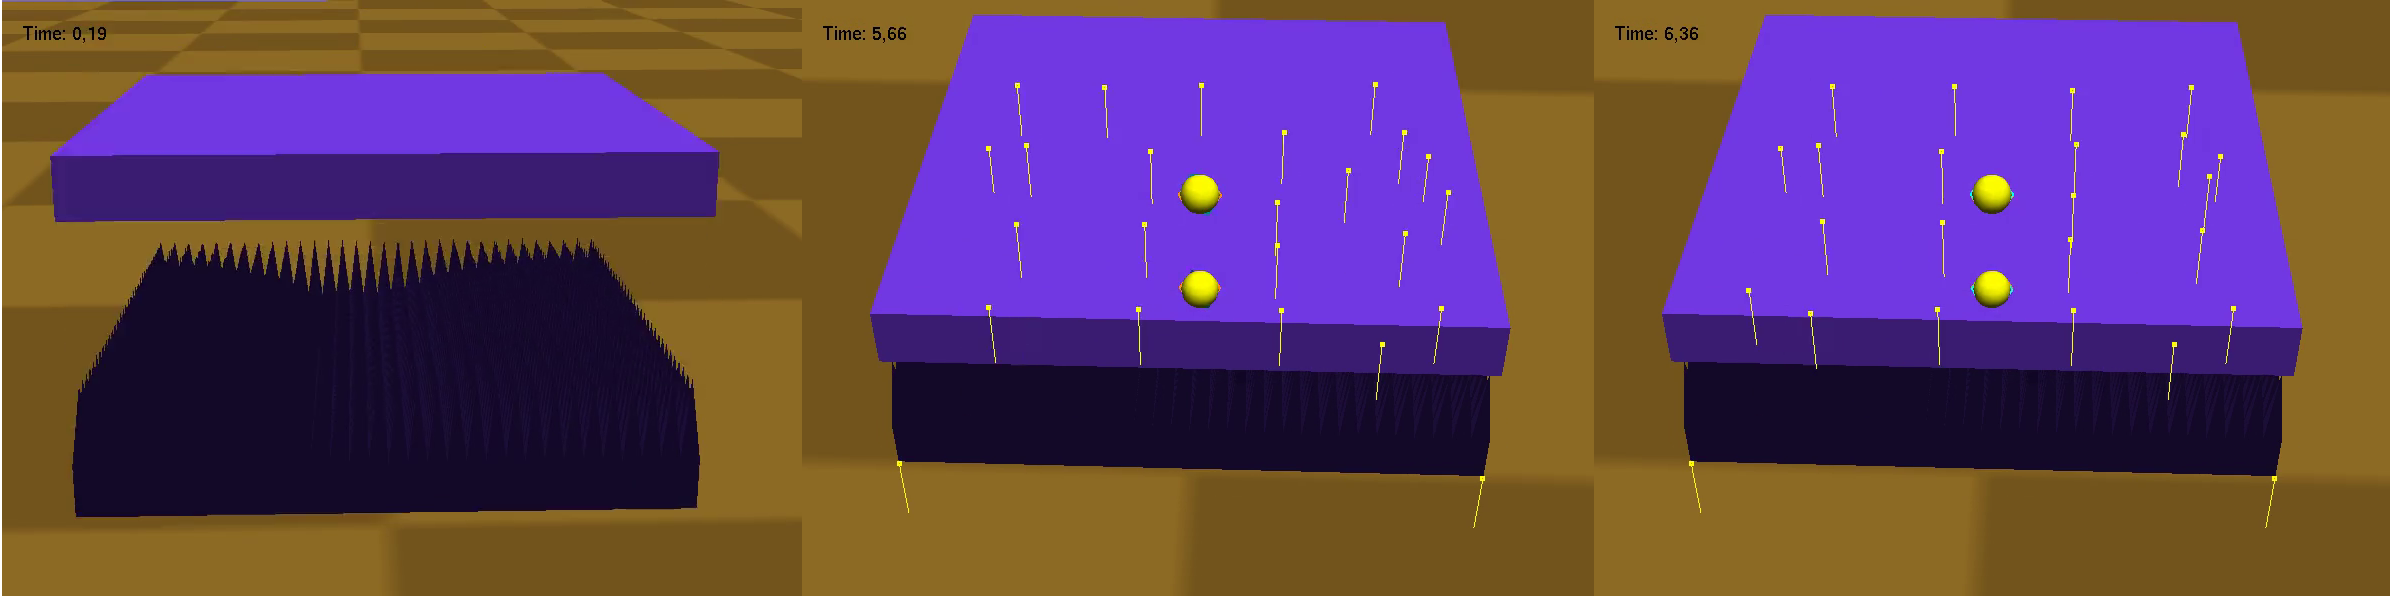
\includegraphics[width=0.95\columnwidth]     {images/ssoch/clustering}
        \caption{Illustrating two contact clustering methods on a 2,000-spike ``spiky block''. Left: hierarchical clustering.  Right: $k$-means clustering. Centers of pressure are draw}
        \label{fig:clustering}
        \end{center}
\end{figure}


\subsection{Contact stability metrics}

In the following section are introduced the metrics used in this work for evaluating the stability of contact points and contact forces at a fine granularity during the simulation of grasping.  These metrics correspond to the position, normal, and force dimensions of point contact models used in classical grasp analysis, which forms the basis of most grasp planning techniques.

\subsubsection{Contact Force Variation}

At equilibrium, we expect the contact forces exerted on the objects to be as close to constant as possible. Our first measurement penalizes fluctuations and spikes in force at an (ostensible) equilibrium state. 

The resultant contact force exerted on body $i$  is $f_i \equiv \int_{x\in S_i(q)} \rho_i(x) dx$, which the simulator approximates by a finite set of contact forces.  The contact force smoothness index measures the normalized standard deviation of resultant forces. (It may be possible to also include resultant torques  $m_i \equiv \int_{x\in S_i(q)} (x-o_i) \times \rho_i(x) dx$ but these are highly correlated to forces for most grasps so we ignore them.) 

Over a span of time $t$ where the object should be held in equilibrium by the physical hand, we measure the quantities $\sqrt{\|Var[f_i(t)]\|_F} / E[\|f_i(t)\|]$ for all bodies $i$ in the set $C$ of bodies touching the object.  Here $\|\cdot\|_F$ denotes the matrix Frobenius norm. We then report the final score (0 being best):
\begin{equation}
S_{cf} \equiv \frac{1}{|C|} \sum_{|i\in C|} \sqrt{\|Var[f_i(t)]\|_F} / E[||f_i(t)||].
\end{equation}

\subsubsection{Contact position and normal variation}
The second and third scores measure the stability of contact positions and normals during an equilibrium grasp.  A simulator generates a set of point contacts at location $x_1,\ldots,x_k$ and their corresponding normals $n_1,\ldots,n_k$ ($k$ varying by time step).  The scores measure the fluctuations of the average contact position $\hat{x}_i$ on body $i$ and average contact normal $\hat{n}_i$ over time (0 being best).

The equations are as follows:
\begin{equation}
S_{cp} \equiv \frac{1}{C} \sum_{|i\in C|} \sqrt{\|Var[\hat{x}_i(t)]\|_F}
\end{equation}
\begin{equation}
S_{cn} \equiv \frac{1}{C} \sum_{|i\in C|} \sqrt{\|Var[\hat{n}_i(t)]\|_F}
\end{equation}

An example of these results for the spiky plane example is given in Fig.~\ref{fig:SpikyStability}.

\begin{figure}
\centering
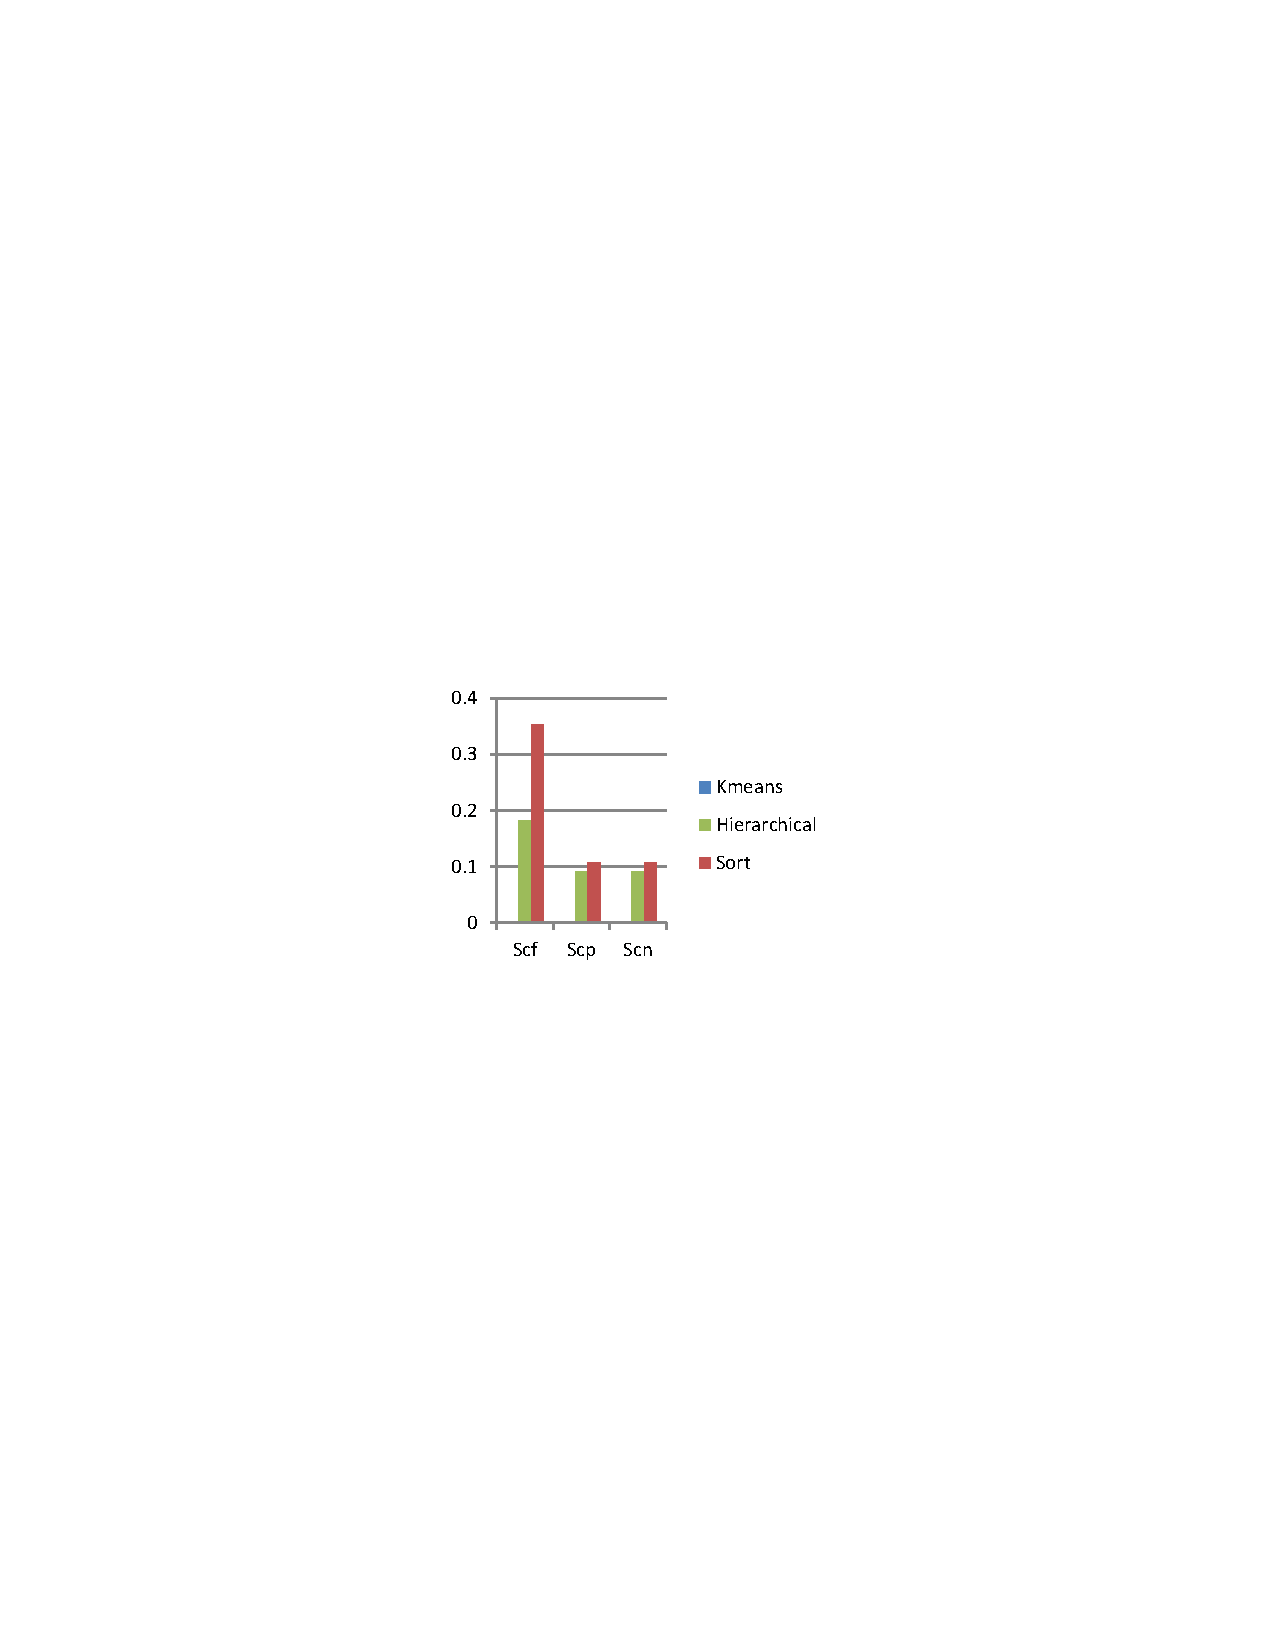
\includegraphics[width=0.6\columnwidth]{images/ssoch/spiky_metrics.pdf}
\caption{Contact stability metrics $S_{cf}$, $S_{cp}$, and $S_{cn}$ over the spiky plane example of Fig.~\ref{fig:clustering} for various clustering methods. K-means leads to almost imperceptible instability (~$1E-17$ for all three indices)}
\label{fig:SpikyStability}
\end{figure}


\subsection{Experiments}
\label{experiments5}

Experiments are performed both with a RightHand Robotics' ReFlex Hand and Pisa/IIT SoftHand.  A set of grasps with varying degrees of robustness are designed by human inspection and tested on a set of physical objects and their simulated counterparts.

\begin{table}[hbt]
   \begin{center}
   \begin{tabular}{| c | c | c |}
   \hline
   Object & Weight & Size \\
   \cline{1-3}
   Hammer					& 480 g   	& 290mmX35mmX95mm      \\\hline
   Spray Bottle (no cap)	& 703.5 g   & 220mmX120mmX40mm      \\\hline
   Spray Bottle (with cap)	& 726 g   	& 270mmX120mmX40mm      \\\hline
   Ketchup				& 948.6 g   & 195mmX100mmX70mm   \\\hline
   Pasta Box				& 487g      & 120mmX19mmX72mm      \\\hline
   \end{tabular}
   \end{center}
   \caption{Weight of all the objects and approximate dimensions}
   \label{table:object}
\end{table}


For the two hands, a series of grasps are selected for each object in the set:
\emph{hammer, ketchup bottle, spray bottle} and a \emph{pasta box}.
The \emph{hammer} and the \emph{pasta box} are modeled by hand. The rest of the objects have been scanned using a \emph{Makerbot Digitizer}. The results and details of the mesh reconstruction are shown and detailed in Fig. \ref{meshes}.
Dimensions are given in Tab.~\ref{table:object}.
We assume an approximate mass distribution for the \emph{hammer}, and for the mass of the the rest of the objects.
In all the experiments, the objects are laying on a table.


Human-chosen grasps are selected in order to have a selection of robust grasps, non-robust grasps, and failed grasps as described in Tab.~\ref{table:grasp}. Robust grasps tolerate small variations in the object pose and disturbance forces. Non-robust grasps succeed some of the time, but do not always tolerate such variations.  Failed grasps fail consistently.  

The hands and the table are marked with fiducial markers, and their position and orientation are recorded for each grasp via a Microsoft Kinect camera. The objects are placed on the table in a known pose, and the grasps illustrated in Fig. \ref{hammer}, \ref{heinz_bottle} and \ref{spray} are performed. For every nominal grasp pose, the hand has been positioned manually on the desired configuration via the gravity compensation control of the \emph{Baxter} robot. A set of $6$ trials is performed for each grasp, and grasp scores are averaged over the attempts over three indices:

\begin{table}[hbt]
   \begin{center}
   \begin{tabular}{| p{1.5cm}  | c | c | p{2.5cm} | c |}
   \hline
   Object   & Pose  & Effort &  Grasp Position  & Preshape \\
   \cline{1-5}
   Hammer					& P1   		&	0.3	& 	Handle	& 	0   \\\hline
   Hammer					& P2   		&	0.3	& 	CoG	& 	0   \\\hline
   Hammer					& P3   		&	0.3	& 	Head	& 	0.5 \\\hline
   Spray Bottle (no cap)	& P1   		&	0.2	&   Low (spray facing outside) 	&	0	\\\hline
   Spray Bottle (no cap)	& P2   		&	0.2	&   High  (spray facing outside)  	&	0	\\\hline
   Spray Bottle (no cap)	& P3   		&	0.2	&   Low (spray facing inside)  	&	0	\\\hline
   Spray Bottle (no cap)	& P4   		&	0.2	&   High (spray facing inside)    			&	0	\\\hline   
   Spray Bottle (with cap)	& P1   		&	0.2	&   High   	&	0	\\\hline
   %Ketchup				& P1   		&	0.3	&   Cap   	&	1.5	\\\hline %got experiment, but not simulation
   Ketchup				& P1   		&	0.3	&   Cap   	&	1.5	\\\hline
   Ketchup				& P2   		&	0.3	&   Under cap ridge   	&	1.3	\\\hline
   Ketchup				& P3   		&	0.2	&   Lateral ridge   	&	0	\\\hline
   Ketchup				& P4   		&	0.2	&   Above lateral ridge   	&	0	\\\hline
   Pasta Box				& P1   		&	N/A	&   Top, parallel   	&   N/A	\\\hline
   Pasta Box				& P2   		&	N/A	&   Top, tilt along yaw   	&	N/A \\\hline
   Pasta Box				& P3   		&	N/A	&   Side   	&   N/A	\\\hline   
   
   \end{tabular}
   \end{center}
   \caption{Grasp configuration}
   \label{table:grasp}
\end{table}


\begin{figure}[!hbt]
\begin{center}
        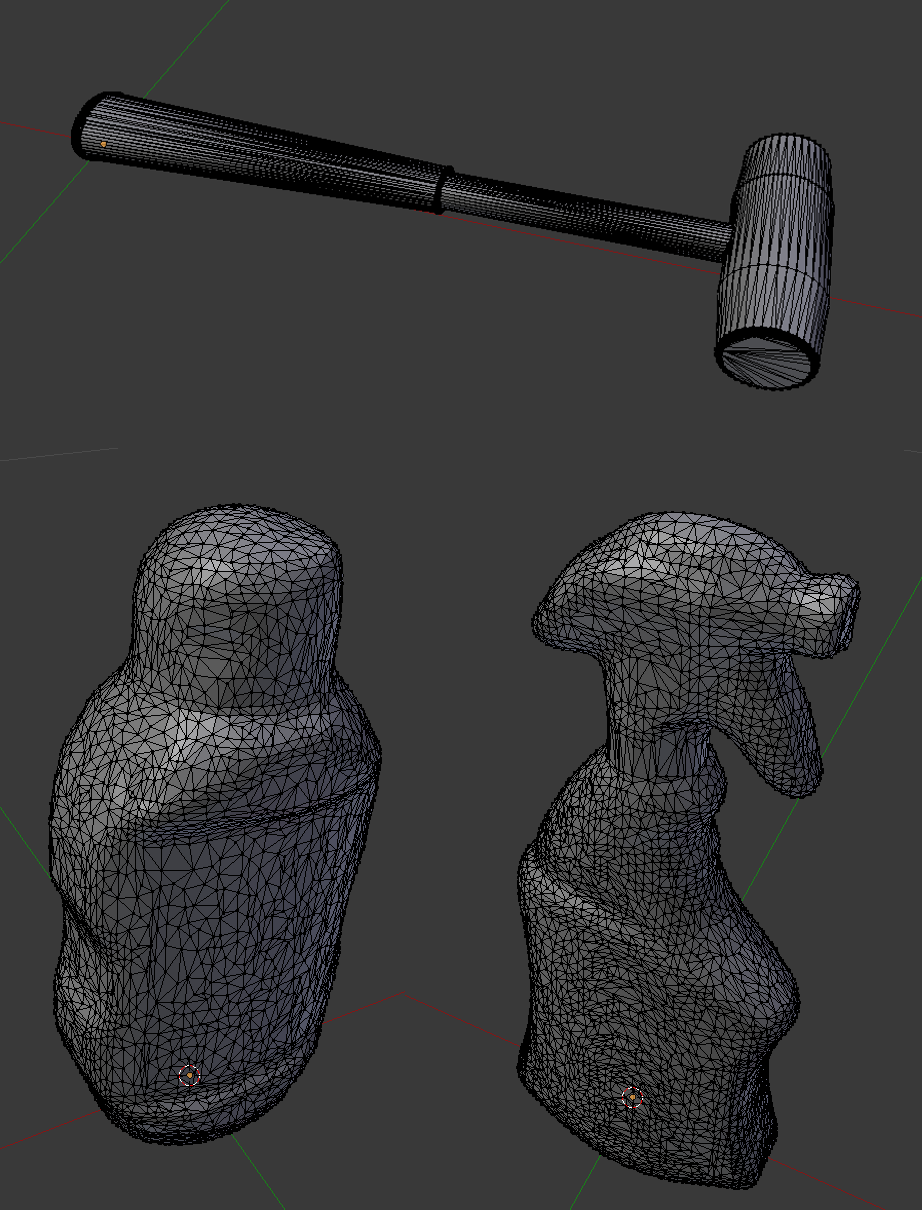
\includegraphics[width=0.6\columnwidth]     {images/ssoch/meshes}
        \caption{The 3d laser range scans are reconstructed using Poisson surface reconstruction, and the number of faces of the mesh is then reduced using Quadric Edge Collapse Decimation. All the meshes have a number of faces between $8000$ and $12000$. As a last step, the bottom of the object is manually cropped to a flat surface.}
        \label{meshes}
        \end{center}
\end{figure}

\begin{figure}[!hbt]
\begin{center}
        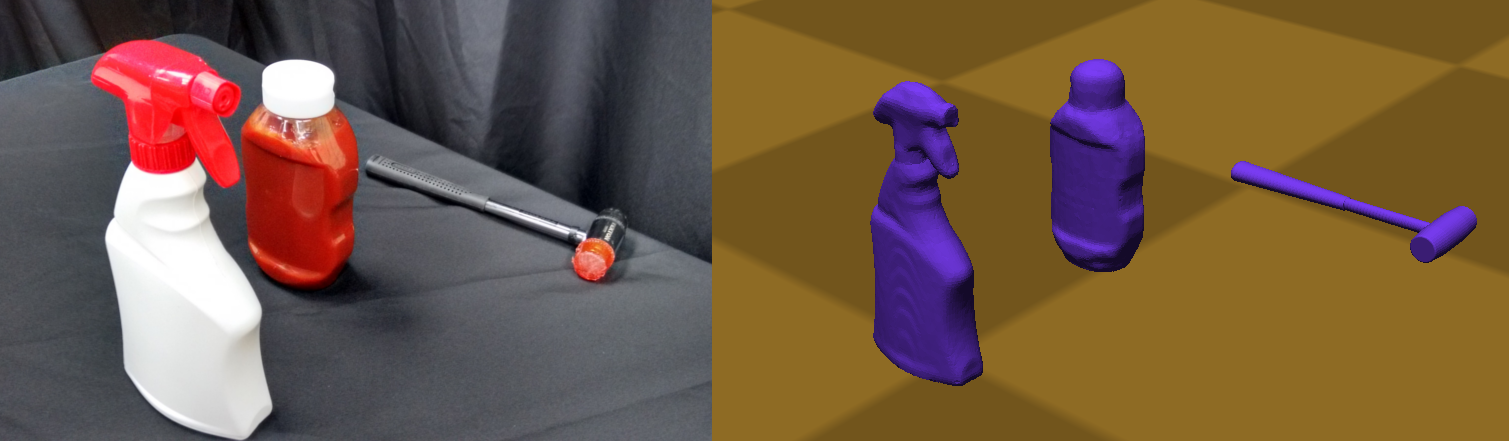
\includegraphics[width=0.95\columnwidth]     {images/ssoch/objects}
        \caption{comparison side by side of the real objects and the 3d scanned}
        \label{objects}
        \end{center}
\end{figure}



\begin{itemize}
\item \textbf{$S1$ object pose deviation}. This is designed in order to be performed easily by eye without complicated measurements attempts. As it can be seen in \ref{real_score} it is practically useful only in the \emph{hammer} set of grasps, because of the advantageous lever the CoM has on the grasp. In the bidimensional case, the index uniformly discretizes the possible swing angle of the hammer in $3$ regions, with scores $1$, $0.6$ and $0.3$. The score will be $0$ in case of an unsuccessful grasp.
\item \textbf{$S2$ the normalized number of fingers in contact}. For the Reflex Hand, the index can assume values $1$ for a three-fingers grasp and $0.5$ for a two fingers grasp. For the Soft Hand, the index can assume values $1$,$0.75$,$0.5$ and $0.25$.
\item \textbf{$S3$ ability to resist perturbation}. By applying a shaking motion on the hand of the robot, we check if one of the previous indices changes in value as a consequence of the perturbation, in which case the score will be $0.6$. In case of a dropped object as a consequence of the perturbation, the score will be $0.3$.
\end{itemize}


\begin{figure}[!hbt]
\begin{center}
        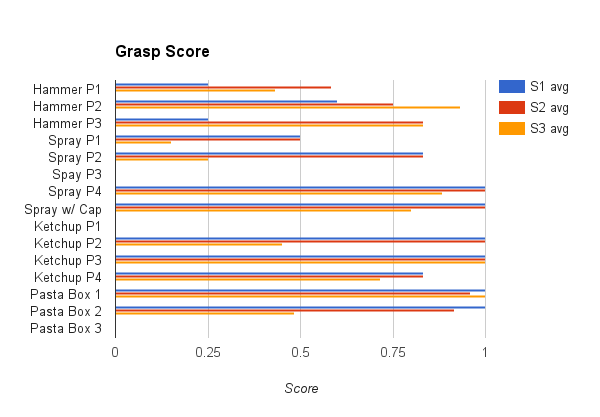
\includegraphics[width=0.95\columnwidth]     {images/ssoch/real_score}
        \caption{Grasp scores for physical experiments. On the \emph{x} axis, $1-3$ are for \emph{hammer-P1} to \emph{hammer-P3}, $4-7$ are for \emph{spray-P1} to \emph{spray-P4}, while score $8$ is for \emph{spray-full-P1}, $9-13$ are for \emph{Ketchup-P1} to \emph{Ketchup-P5}}
        \label{real_score}
        \end{center}
\end{figure}

The grasp procedure for the \emph{Reflex Hand} consists in simultaneously closing each finger until the motor's effort threshold is met, at which point the finger is stopped. For the \emph{Soft Hand}, the fingers close simultaneously until the nominal torque limit of the single actuator is reached. To check if the grasp is successful, the object is then raised. If successfully raised, the robustness of the grasp is checked by shaking the gripper by hand.


\begin{figure}[!hbt]
\begin{center}
        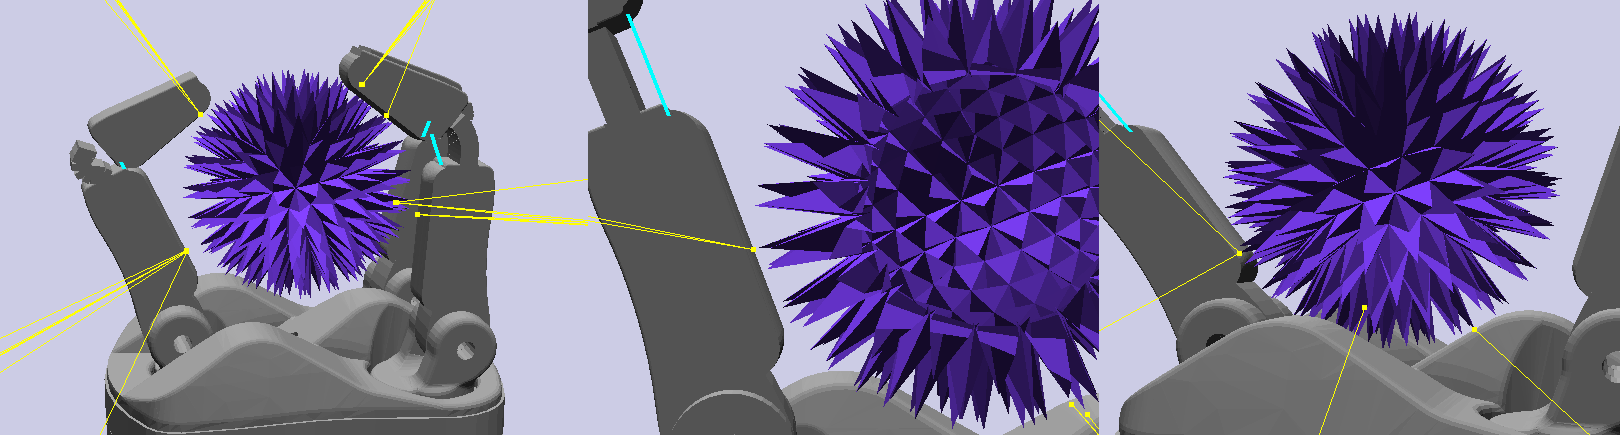
\includegraphics[width=0.95\columnwidth]     {images/ssoch/preshrink}
        \caption{Since the \emph{BLEM} method works by expanding the meshes via Minkowski dilation, a preshrink method was introduced so that the boundary layer added to a preshrunk mesh will sum up to the approximate size of the original mesh. In figure, from left to right, a $5mm$ boundary layer shows gaps between the hand and the object, a $1mm$ boundary layer, and a $1mm$ layer with preshrink. }
        \label{Preshrink}
        \end{center}
\end{figure}


The grasp is then performed in simulation.
We simulate the \emph{Reflex Hand} using \emph{Klamp't} v$0.6.2$, and the \emph{Soft Hand} using \emph{Gazebo} v$4.0$ with a preliminary version of the \emph{Soft Hand plugin}~\cite{Rosales15SHP}.
The \emph{Gazebo} simulator is tested against our patch \cite{Rocchi15GBP} where \emph{BLEM} is used. In Gazebo, the simple contact sorting algorithm is used for contact filtering. The \emph{Klamp't} simulator is tested with  \emph{BLEM} against the default in Open Dynamics Engine \emph{OPCODE}.  In Klamp't examples, we use $k$-means clustering with a maximum of 20 contacts.

The robot's motor parameters, tendon Baumgarte stability constants, and friction parameters were tuned by hand so that the hands would move qualitatively similarly to the real hands, and to be stable both in free space motion and while grasping on a spherical object.  No quantitative calibration procedure was performed.



\begin{figure*}[!!hbt]
\begin{center}
{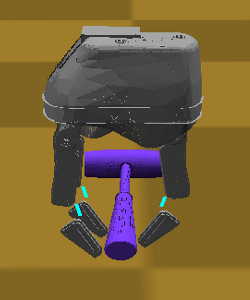
\includegraphics[width=0.11\textwidth]     {images/ssoch/fig/hammer_P1}\label{hammer_P1}}%
{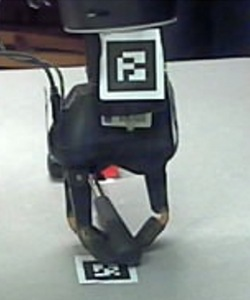
\includegraphics[width=0.11\textwidth]     {images/ssoch/fig/hammer_p1_1}\label{hammer_p1_1}}
{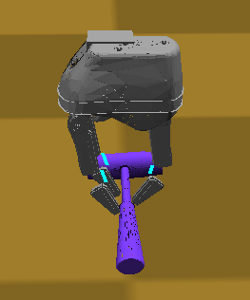
\includegraphics[width=0.11\textwidth]     {images/ssoch/fig/hammer_P2}\label{hammer_P2}}%
{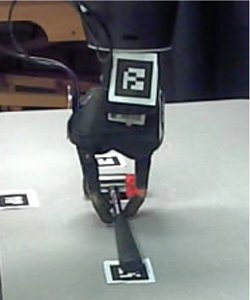
\includegraphics[width=0.11\textwidth]     {images/ssoch/fig/hammer_p2_1}\label{hammer_p2_1}}
{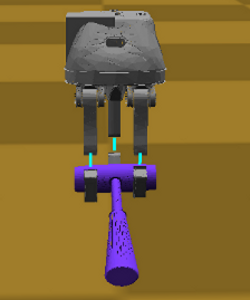
\includegraphics[width=0.11\textwidth]     {images/ssoch/fig/hammer_P3}\label{hammer_P3}}%
{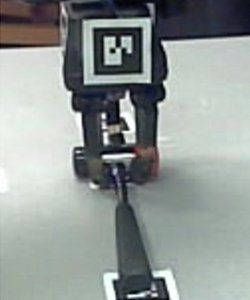
\includegraphics[width=0.11\textwidth]     {images/ssoch/fig/hammer_p3_1}\label{hammer_p3_1}}
        \caption{Comparison between simulation and experiment: \emph{Hammer-P1}, \emph{Hammer-P2}, \emph{Hammer-P3}}
        \label{hammer}
        \end{center}
\end{figure*}


\begin{figure*}[!!hbt]
\begin{center}
{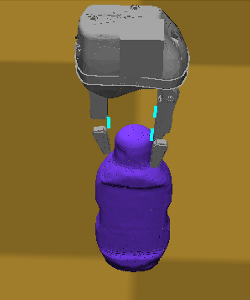
\includegraphics[width=0.11\textwidth]     {images/ssoch/fig/heinz_P1}\label{heinz_P1}}%
{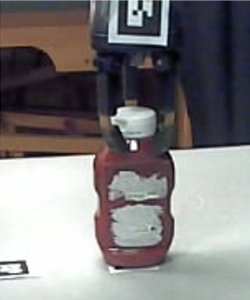
\includegraphics[width=0.11\textwidth]    {images/ssoch/fig/heinz_p1_1}\label{heinz_p1_1}}
{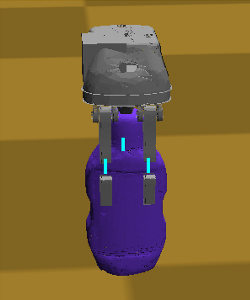
\includegraphics[width=0.11\textwidth]{images/ssoch/fig/heinz_P2}\label{heinz_P2}}%
{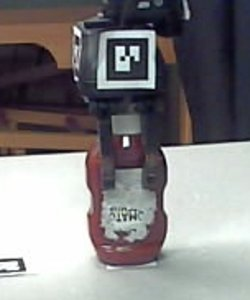
\includegraphics[width=0.11\textwidth]{images/ssoch/fig/heinz_p2_1}\label{heinz_p2_1}}
%{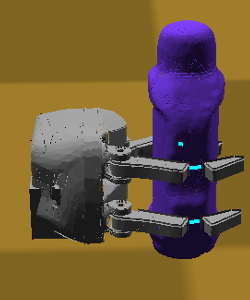
\includegraphics[width=0.09\textwidth]{images/ssoch/fig/heinz_P3}\label{heinz_P3}}%
%{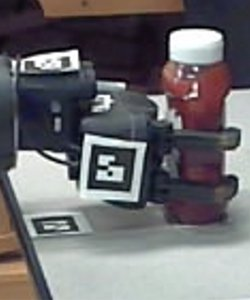
\includegraphics[width=0.09\textwidth]    {images/ssoch/fig/heinz_p3_1}\label{heinz_p3_1}}
{ 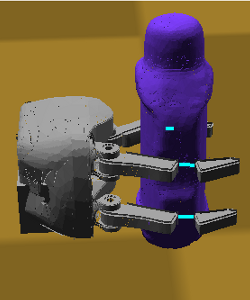
\includegraphics[width=0.11\textwidth]     {images/ssoch/fig/heinz_P4}\label{heinz_P4}}%
{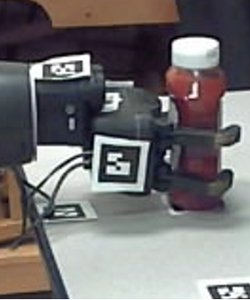
\includegraphics[width=0.11\textwidth]{images/ssoch/fig/heinz_p4_1}\label{heinz_p4_1}}
{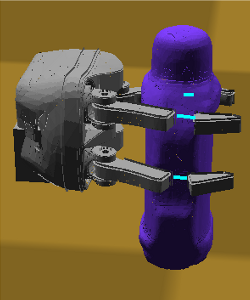
\includegraphics[width=0.11\textwidth]{images/ssoch/fig/heinz_P5}\label{heinz_P5}}%
{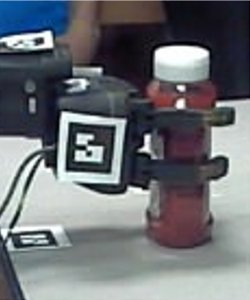
\includegraphics[width=0.11\textwidth]{images/ssoch/fig/heinz_p5_1}\label{heinz_p5_1}}
        \caption{Comparison between simulation and experiment: \emph{Ketchup-P1}, \emph{Ketchup-P2}, \emph{Ketchup-P3}, \emph{Ketchup-P4}}
        \label{heinz_bottle}
        \end{center}
\end{figure*}


\begin{figure*}[!!hbt]
\begin{center}
{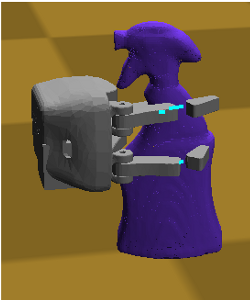
\includegraphics[width=0.09\textwidth]     {images/ssoch/fig/spray_full_P1}\label{spray_full_P1}}%
{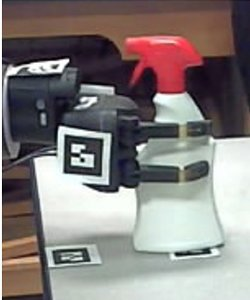
\includegraphics[width=0.09\textwidth]     {images/ssoch/fig/spray_full_p1}\label{spray_full_p1}}
{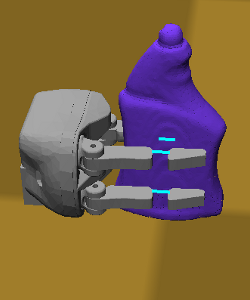
\includegraphics[width=0.09\textwidth]{images/ssoch/fig/spray_P1}\label{spray_P1}}%
{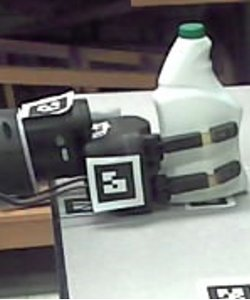
\includegraphics[width=0.09\textwidth]{images/ssoch/fig/spray_p1}\label{spray_p1}}
{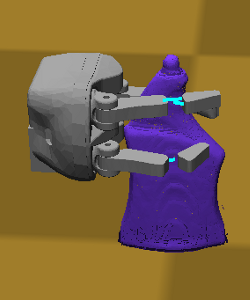
\includegraphics[width=0.09\textwidth]{images/ssoch/fig/spray_P2}\label{spray_P2}}%
{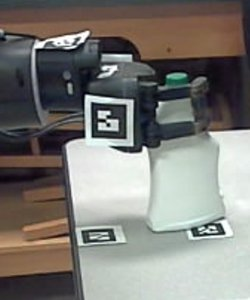
\includegraphics[width=0.09\textwidth]{images/ssoch/fig/spray_p2}\label{spray_p2}}
{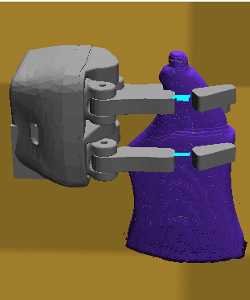
\includegraphics[width=0.09\textwidth]{images/ssoch/fig/spray_P3}\label{spray_P3}}%
{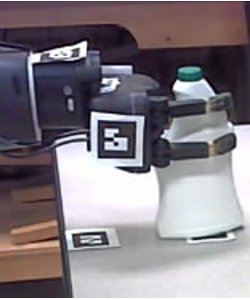
\includegraphics[width=0.09\textwidth]{images/ssoch/fig/spray_p3}\label{spray_p3}}
{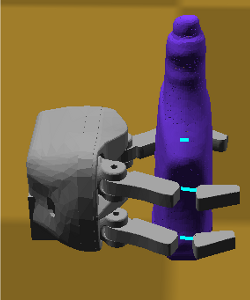
\includegraphics[width=0.09\textwidth]{images/ssoch/fig/spray_P4}\label{spray_P4}}%
{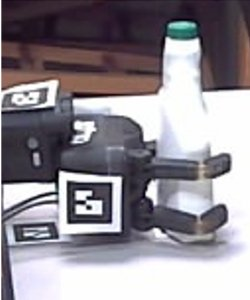
\includegraphics[width=0.09\textwidth]{images/ssoch/fig/spray_p4}\label{spray_p4}}
        \caption{Comparison between simulation and experiment: \emph{Spray Bottle (with cap)}, \emph{Spray Bottle (no cap) - P1}, \emph{Spray Bottle (no cap) - P2}, \emph{Spray Bottle (no cap) - P3}, \emph{Spray Bottle (no cap) - P4}}
        \label{spray}
        \end{center}
\end{figure*}


\begin{figure*}[!!hbt]
\begin{center}
{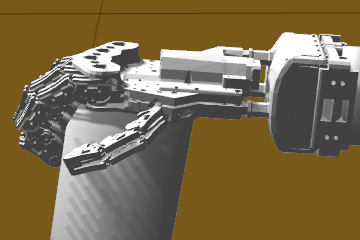
\includegraphics[height=0.12\textwidth]     {images/ssoch/fig/kh_changes/softhand_p1_simu01}}%
{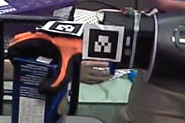
\includegraphics[height=0.12\textwidth]     {images/ssoch/fig/kh_changes/softhand_p1_grasp}}
{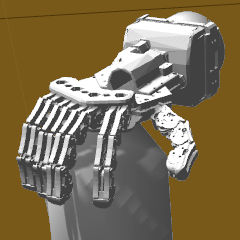
\includegraphics[height=0.12\textwidth]     {images/ssoch/fig/kh_changes/softhand_p2_simu01}}%
{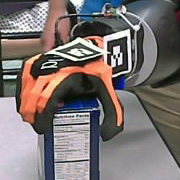
\includegraphics[height=0.12\textwidth]     {images/ssoch/fig/kh_changes/softhand_p2_grasp}}
{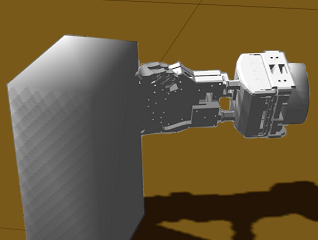
\includegraphics[height=0.12\textwidth]     {images/ssoch/fig/kh_changes/softhand_p3_simu01}}%
{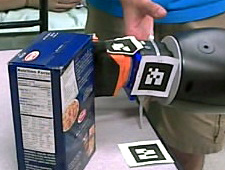
\includegraphics[height=0.12\textwidth]     {images/ssoch/fig/kh_changes/softhand_p3_grasp}}
        \caption{Comparison between simulation and experiment: {\em Pasta Box - P1}, {\em Pasta Box - P2}, and {\em Pasta Box - P3}.}
        \label{pasta_box}
        \end{center}
\end{figure*}


The simulation procedure is as follows:
\begin{itemize}
\item The object and hands are spawned in the pregrasp and preshape configuration,
\item As in the physical hardware, the hands are closed until an actuator force threshold is reached.
\item The hand is lifted by 10cm,
\item The grasp is perturbed by commanding jerking movements of the wrist,
\item Finally the hand opens to drop the object.
\end{itemize}

\begin{figure*}
\centering
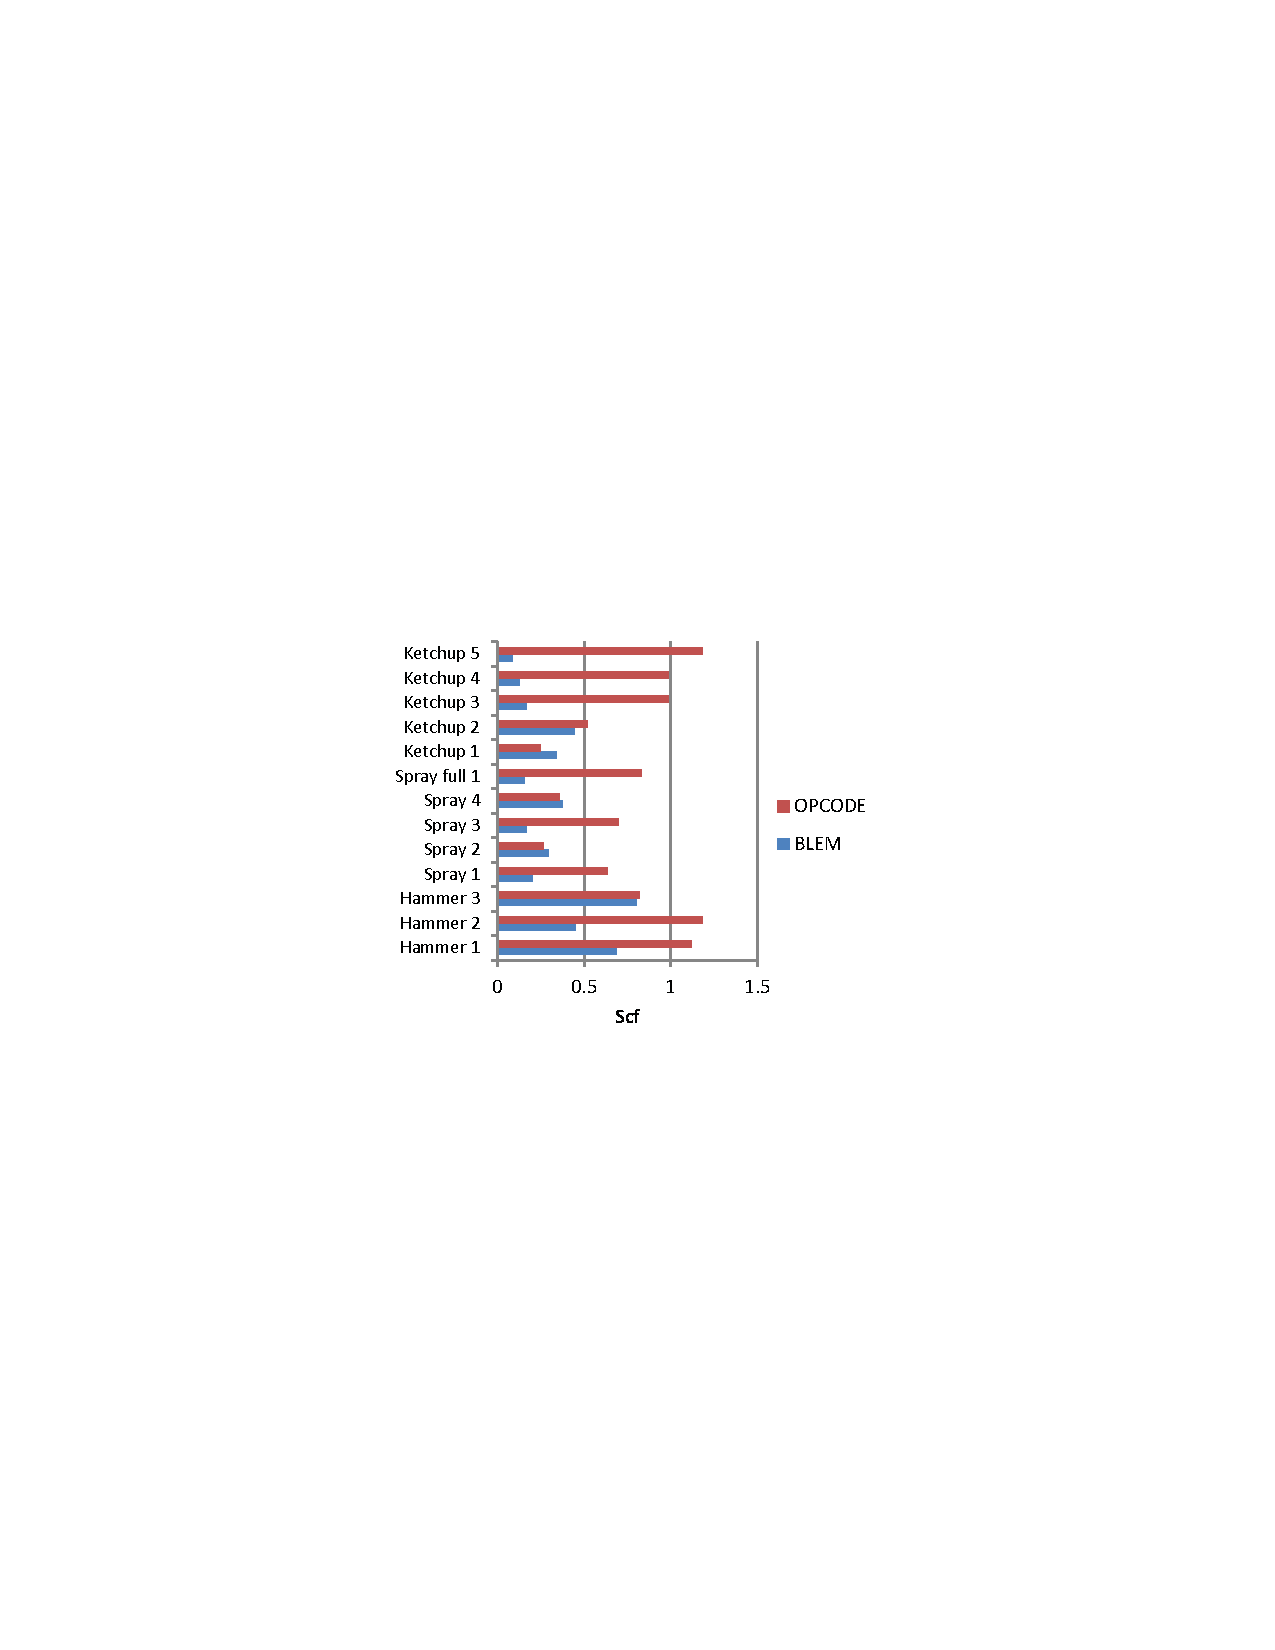
\includegraphics[width=0.32\textwidth]{images/ssoch/scf_metrics.pdf}
\includegraphics[width=0.32\textwidth]{images/ssoch/scp_metrics.pdf}
\includegraphics[width=0.32\textwidth]{images/ssoch/scn_metrics.pdf}
\caption{Metrics $S_{cf}$, $S_{cp}$, and $S_{cn}$ over the simulated grasp set. Lower numbers are better.}
\label{fig:AllMetrics}
\end{figure*}

Fig.~\ref{fig:AllMetrics} illustrates the results of the contact stability indices between BLEM and OPCODE contact generation. It can be observed BLEM leads to higher stability in general, most strikingly for the contact normal metric.

\begin{table}[hbt]
   \begin{center}
   \begin{tabular}{| c | c  c | c c |}
   \hline
   Grasp & Grasped & Dropped & Grasped & Dropped\\
   \hline
    {\bf ReFlex} & \multicolumn{2}{c|}{{\bf ODE / BLEM}} & \multicolumn{2}{c|}{{\bf ODE / OPCODE}} \\
   \cline{1-5}
   Hammer 1	    & Y & Y & Y & {\bf N} \\
   Hammer 2	    & Y & Y & Y & Y \\
   Hammer 3	    & Y & Y & Y & {\bf N} \\
   ~Spray 1+	& Y & Y & Y & {\bf N} \\
   ~Spray 2+	& Y & Y & Y & {\bf N} \\
   ~Spray 3*	& Y & Y & Y & Y \\
   Spray 4	& Y & Y & Y & {\bf N} \\
   Spray Full 1	& Y & Y & Y & Y \\
   ~Ketchup 1*	& Y & Y & {\bf N} & -- \\
   Ketchup 2	& Y & Y & {\bf N} & -- \\
   Ketchup 3	& Y & Y & Y & {\bf N} \\
   Ketchup 4	& Y & Y & Y & {\bf N} \\
   \hline
   {\bf SoftHand} & \multicolumn{2}{c|}{{\bf Gazebo / BLEM}} & \multicolumn{2}{c|}{{\bf Gazebo / OPCODE}} \\
   \hline
   Pasta Box 1  & Y & Y & X & Y \\
   Pasta Box 2+ & Y & Y & X & Y \\
   Pasta Box 3* & N & -- & N  & -- \\
   \hline
   \end{tabular}
   \end{center}
   \caption{Success rates of ReFlex grasps (top) and SoftHand grasps (bottom) in simulation.  Asterisks indicate failed grasps on physical experiments. The plus sign indicates non robust grasps on physical experiments.  An entry of X  indicates variability for the same initial conditions.}
   \label{table:GraspSuccess}
\end{table}

Tab.~\ref{table:GraspSuccess} illustrates the results of simulations. 12/12 successful grasps were reliably grasped by BLEM and 9/12 were grasped by OPCODE. In all successful grasps, the object was securely held through perturbations.  In the two ODE/OPCODE failure cases, the hand  penetrated completely through the object without contact.  In the two Gazebo/OPCODE unreliable grasp cases, we observed  nondeterminism in the simulator which caused the grasp to fail in approximately 1/3 of simulation trials, even with the exact same initial conditions.

Perhaps more worrisome is the result that ODE/OPCODE did not successfully release the grasped object in 7/9 successful grasps.  This is explained by major interpenetration artifacts, in which the object gets ``stuck'' on the robot's finger and cannot be let go (Fig.~\ref{fig:OPCODEArtifact}. 

\begin{figure}
    \centering
    \includegraphics[width=0.25\textwidth]{images/ssoch/opcode-artifact.png}
    \caption{An artifact exhibited in OPCODE causing the object to penetrate and then ``stick'' to the robot's finger.}
    \label{fig:OPCODEArtifact}
\end{figure}

BLEM did not successfully predict 2/3 failed grasps. This likely indicates an improperly calibrated coefficient of friction or absolute grasp force.  This suggests that although stable simulation is crucial for obtaining reasonable predictions, it is still challenging for simulation to accurately discern the boundary of feasible/infeasible grasps without considerable tuning.   An interesting area for future work would be to automatically tune the robot model to obtain a match with physical experiments.

Lastly, computation times during grasp for the \emph{Klamp't} case were similar between BLEM, with $~2.7$ms and OPCODE, with $\sim2.9$ms for each millisecond of simulated time. For Gazebo, the experimental BLEM patch resulted in computation times of $\sim2.4$ms against $\sim1.6$ms of OPCODE for each millisecond of simulated time. All measurements were taken on an Intel Core i5-4460 CPU @3.2HGz.

\subsection{Conclusions}
A series of simulation stability and fidelity criterion have been established. They have been tested on two different compliant and underactuated hardware platforms, the \emph{RightHand Robotics' Reflex Hand} and the \emph{Pisa/IIT SoftHand}. A set of grasps has been performed on the physical hardware using $4$ different objects of different shapes and characteristics, in different grasping scenarios, and then validated using \emph{Klamp't} and \emph{Gazebo}, using different techniques for \emph{contact clustering} and \emph{contact generation}. The experimental results show that  simulations performed with the \emph{BLEM} \emph{contact generation} algorithm and the \emph{k-means clustering} contact filtering algorithm have the highest stability indices, and also exhibit the fewest artifacts.

\section{Simulating Compliant Humanoid Robots}
\let\thefootnote\relax\footnotetext{based on \cite{Hoffman2014yarp}}
\subsection{Simulators as Abstractions to the Physical Hardware}
\subsubsection{YARP Plugins for the Gazebo Simulator}
\subsubsection{Real-Time Simulation of Robotic Systems}

\section{Simulating Grasps}
\subsection{Stable Simulation of Underactuated and Compliant Hands}
\let\thefootnote\relax\footnotetext{based on \cite{Rocchi2016-jq}}

\chapter{Whole-Body Control}
\def\q{\mathbf{q}}
\def\dq{\mathbf{\dot{q}}}
\def\J{\mathbf{J}}
\def\A{\mathbf{A}}
\def\B{\mathcal{B}}
\def\C{\mathcal{C}}
\def\T{\mathcal{T}}
\def\W{\mathbf{W}}
\def\b{\mathbf{b}}
\def\I{\mathbf{I}}
\def\x{\mathbf{x}}
\def\dx{\mathbf{\dot{x}}}
\def\e{\mathbf{e}}
\def\de{\mathbf{\dot{e}}}
\def\w{\mathbf{w}}

\externaldocument{architecture}

\todo{ADD material from the original ICRA work}
The field of whole-body planning and control tries to find the solution to the problem of executing one or more task at the same time, while exploiting the capabilities of the entire body of redundant, floating-based robots in multi-contact scenarios with the environment.

%The problem entails modeling and controlling systems with hybrid dynamics, encompasses the force distribution problem in multi-contact scenarios, planning for the making and breaking of robot-environment contacts during loco-manipulation tasks, and passes through the optimization of the robot resources to maximally exploit the kinematic structure and the dynamics of the robot and the task.
%Related problems to the whole-body control are of mechatronic(how to design an agile and robust robot), and computational origin: the joint design (compliant, rigid), as well as the search for designs to obtain reliable low-level torque control, and in the case of compliant joints, performant low-level position controls, and under the computation point of view, fast numerical methods, software and hardware architectures able to accomplish high frequency, reliable control.
%Other than being a research problem, it still is a technological problem to either implement, simulate and control highly redundant robots, such as humanoid robots. Not only the prices for building such robots are still very high, being the assembly of robots ironically man-made (with a very interesting and ambitious vision from Boston Dynamics to 3d-print the robots of the future), but the technological problems range from the problem of building a reliable, high-throughput and high-bandwidth communication network between the sensors, actuators and controllers, to obtaining reliable torque sensing at the joint level, to building agile robots which are also resilient, and of course to the computational limitations one encounters when writing control algorithms for highly redundant robots.

Several and different approaches are being investigated by the research community, such as optimization, inverse dynamics, inverse kinematics with dynamic filters and admittance control. \todo{how long is this so far? I could also go in more detail on the state of the art of several kind of control? Or briefly on the problem in general, and more in detail on the kinematic problem}.

Inverse Kinematics (IK) is a fundamental component for a vast number of application in robotics. In particular, kinematic control is still a popular choice for high level robot controllers. While the kinematic control problem has been tackled in literature using several different approaches, latest trends both in research and application make use of Quadratic Programming (QP) to obtain a locally optimal solution to the hierarchical constrained IK problem. The interest is in part justified by the need, for practical reasons, to have robust solutions which are hard constrained by the physical limits of the robots, such as joint, torque and self-collision avoidance limits. In this section the theoretical foundations of kinematic control based on QP optimization will be presented, and the formulation of a comprehensive set of tasks and constraints will be provided, according to the capabilities of the developed framework. The kinematic control, and thus the formulation for the tasks and the contraints in the framework will be expressed at the velocity level, meaning the solution of each step of the IK solver will return a displacement $\delta q$ that can be actuated on the physical robot or integrated for kinematic simulation. Some aspects of the IK solver will be described, and the choice of the state-of-art QP solver library \emph{qpOASES} will be motivated. 
The work presented has been been developed as part of the robotic framework \textbf{OpenSoT}, developed at the Italian Institute of Technology \cite{Rocchi2015-is, Fang2015-cr, Ajoudani2014-fs, Lee2014-dg}. The framework has been developed for application to our compliant humanoid robots, in particular to the COMAN~\cite{tsagarakis12} in a compliant inverse kinematics scheme, and WALK-MAN~\cite{Tsagarakis:2016} as part of the high-level control architecture  used in the Darpa Robotics Challenge. The framework consists of a C++ library tailored for the control of hyper-redundant fixed/floating base robot. Experiments and results in the Darpa Robotics Challenge are presented later on in this section, while the software API and tools as will be presented in chapter \ref{architecture}.

%%%%%%%%%%%%%%%%%% INTRO
\section{OpenSoT: a library for Whole-Body Control of Humanoid Robots}
\label{sec:opensot-library}
\begin{wrapfigure}{r}{0.35\textwidth}
  \begin{center}
    \includegraphics[width=0.25\textwidth]{images/openSoT_stickers}
  \end{center}
  \caption{OpenSoT Logo}
\end{wrapfigure}
From a very broad perspective, the inverse kinematics problem is that of mapping task-space objectives into joint-space commands.
Typical techniques to map task-space commands to joint commands can be roughly classified as inverse kinematics or inverse dynamics schemes and can be implemented using a variety of low level controllers.
\textbf{OpenSoT} is a novel whole body motion library developed at the Italian Institute of Technology (IIT), which belongs to the former group: our goal has been to develop a high performance and flexible library that can generate reliably complex and efficient whole body motions.

The \emph{Differential Inverse Kinematics Problem} consists of the determination of the joint trajectories corresponding to a given task for the end-effector in \emph{Operational Space}. This problem is in general highly non-linear, a \emph{closed form} solution may not be available, and may have multiple solutions. In the case in which the robot is \emph{redundant} with respect to the task, that is, the degrees of freedom of the robot are greater than the degrees of freedom required by the specified task,  the IK Problem admits an infinite number of solutions. In case of operational space control, at least a solution is guaranteed to exist if the given goal in operational space belongs to the manipulator \emph{dexterous space}.
Despite the relationship between joint position variables and operational space poses is not linear, the mapping between joint velocity variables and operational space velocities is linear through the robot Jacobian:
\begin{equation}
    \label{eq:differential_kinematics}
    \dx = \J(\q)\dq
\end{equation}
where the Jacobian $\J$ (we will skip the dependency on the actual configuration $\q$ from now on) is expressed from a certain \emph{base link} to a certain \emph{distal link}, and operational space velocities $\dx$ of the \emph{distal link} are expressed in the \emph{base link} reference frame\todo{can be written more clearly. The Jacobian depends on three dimensions, the location of the pole, the location of the frame of reference, and the orientation of the frame of reference. See from the KDL documentation :)}.
A general solution, for the redundant case, of (\ref{eq:differential_kinematics}) is:
\begin{equation}
    \label{eq:differential_inverse_kineamtics}
    \dq_\text{d} = \J^{\dagger}\dx_\text{d} + \left( \I - \J^{\dagger}\J \right)\dq_\text{0}
\end{equation}
where $\J^{\dagger}$ is the \emph{pseudo inverse} of the Jacobian and $\dq_\text{0}$ is an arbitrary joint space velocity. 
This solution allows also for \emph{task prioritization}: 
\begin{equation}
    \label{eq:another_task}
\dq_\text{0} = \J_\text{0}^{\dagger}\dx_\text{0}
\end{equation}
in particular, the solution given by (\ref{eq:differential_inverse_kineamtics}) with (\ref{eq:another_task}), projects the joint velocities of the second task into the null space of the first task removing all the components that would interfere with it \cite{DBLPReferenceRobo2008}. Many other solutions of (\ref{eq:differential_kinematics}) are available in literature \cite{siciliano1991general}. \todo{put solution by Siciliano}. Singularities in the Jacobian, as well as joint velocity limits, are often handled with the \emph{Singularity Robust Inverse} (SRI) \cite{nakamura1990-tp}, \cite{maciejewski1989-jp}.
The problem of this type of schemes is that they do not handle constraints in the form of inequalities. 

To overcome this problem, techniques from the optimization field have been adopted.
We can consider the inverse problem of (\ref{eq:differential_kinematics}) as a Quadratic Programming (QP) problem with linear constraints:
\begin{equation} 
\label{eq:optimization_problem}
\begin{array}{c}
\dq_\text{d} = \underset{\dq}{\operatorname{argmin}} \ \Arrowvert \J \dq-\dx_\text{d} \Arrowvert\\
s.t. \ \mathbf{A}\dq \leq \mathbf{b}
\end{array}
\end{equation}
%where $\Arrowvert \J \dot{\q}-\mathbf{v}_d \Arrowvert = \dot{\q}^\text{T}\J^\text{T}\mathbf{J}\dot{\q} - 2(\J\dot{\q})^\text{T}\mathbf{v}_d+\mathbf{v}_d'\mathbf{v}_d$ is the quadratic cost function that is minimized and $\mathbf{A}\dot{\q} \leq \mathbf{b}$ is a general linear constraint. 
The two most popular families of methods to solve the problem in (\ref{eq:optimization_problem}) are \emph{active set} and \emph{interior point} methods. 
\emph{Active set} methods consider constraints as equalities, in the circumstance when they are active, so that the problem (\ref{eq:optimization_problem}) is transformed in a QP with only equalities. At each iteration the new active set is computed checking for the infeasible constraints.
\emph{Interior point} methods use barrier functions (such as $log$ functions) to penalize the cost function in the region where the bounds are violated and the solution is found by iteratively relaxing the barrier function\todo{it should be the opposite?}.
Even under the optimization point of view, the task prioritization can be handled considering the minimization of the cost function under equality constraints given by the minimization of previous tasks. This technique is commonly referred as \emph{Stack of Tasks} (SoT) \cite{mansard:icar:09}. 

\textbf{OpenSoT} implements the idea of decoupling atomic tasks/constraints descriptions and solvers to execute multiple tasks and achieve complex motion behaviors. It employs a solver implementing a cascade of QP problems, and a set of tasks and constraints in velocity space in order to solve a generic hierarchical inverse kinematics problem on a floating or fixed base robot. The stock IK solver consists on a state machine that hides all the complexity of the underneath QP solver based on a state-of-art library in QP resolution using the active set approach: \emph{qpOASES} \cite{ferreau2013}.
This yields the following features that make the implementation of \textbf{OpenSoT} unique and attractive:   
\begin{itemize}
\item Demonstrates adequate modularity through the separation of task descriptions, control schemes and solvers maximizing customization, flexibility and expandability.  
\item Provides user friendly interfaces for defining tasks, constraints and solvers to promote integration and cooperation in the emerging field of whole-body hierarchical control schemes.
\item Demonstrates computation efficiency to allow for real time performance implementations.
\item Allows ease of use and application with arbitrary robots through the Universal and Semantic Robotic Description Formats (URDF and SRDF).
\end{itemize}
The reliability and robustness of \textbf{OpenSoT} framework has been proved during the DRC Finals since it has been used by the WALK-MAN team, to perform all the manipulation tasks involving \emph{whole-body} motions while taking into account various type of constraints. During the development period, the \textbf{OpenSoT} framework allowed the fast evaluation of different formulations of the whole-boby control problem in order to optimally solve the tasks of the competition, thusly demonstrating the benefits of a flexible high-level framework in robotics rapid application development. 
The architecture of \textbf{OpenSoT} encourages collaboration and helps integration and code maintenance.

%\todo{should I integrate some of this stuff here?}
%Recent approaches make use of Quadratic Programming (QP) Optimization that makes also possible to specify linear constraints for the IK to affect the solution:
%\begin{equation}
%\begin{array} {ccc}
%    \dq_d  = & \underset{ \dq }{ \text{argmin} } & \left\| \J_n \dq - \dx_\text{n,d} \right\| + \lambda \left\| \dq \right\| \\
%    & {s.t.} & \A_1 \dq = \A_1 \dq_1 \\
%    & &  \vdots \\
%    & & \A_{n-1} \dq = \A_{n-1} \dq_{n-1} \\
%    & & \A_{c,1}\dq \leq \b_{c,1} \\
%    & & \vdots \\
%    & & \A_{c,n}\dq \leq \b_{c,n}
%\end{array}
%\label{eq:sot_full}
%\end{equation}
%where $\A$ matrices and $\b$ vectors are constraints.
%In \eqref{eq:sot_full}, priorities are taken into account considering the previous solutions $\dq_i, \; i < n$ and constraints of the type {$\mathbf{A}_i \dq = \mathbf{A}_i \dq_i, \; \forall i < n$},  so that the optimality of all higher priority tasks is not changed by the current solution \cite{mansard:icar:09}. The second term in the cost function of \eqref{eq:sot_full} permits to handle kinematics singularities in order to avoid high joint velocities \cite{nakamura1990-tp}. A similar structure can be used to solve the IK problem at the acceleration level.

%Many tasks and constraints have been presented in literature for the framework depicted in \eqref{eq:sot_full}, examples are: joint limits, joint velocity limits, self collision avoidance \cite{kanehiro2008local}, Cartesian velocity limits, minimum joint acceleration \cite{flacco2012-cr} and \emph{Capture Point} \cite{ ramos-humanoid-14} for humanoid robots. In particular, joint limits and joint velocity limits are fundamental when working with real robotic hardware.  

\subsection{Related Work}
\label{sec:related_work_opensot}
Many approaches to solve the IK problem are presented in the literature and most of them address the singularity problem through Tikanov regularisation, with approaches similar to the \emph{Singularity Robust Inverse} (SRI), but lack the possibility to specify constraints, whereas the aforementioned QP formulation allows for an elegant formulation of the IK problem considering linear constraints\todo{write this more clearly?}.
\textbf{OpenSoT} is thus inspired by the \emph{Stack of Tasks}, where the stock IK solver is based on QP (Quadratic Programming) optimization with the possibility to specify \emph{hard} \cite{kanoun2009prioritizing} and \emph{soft} \cite{chiacchio1991closed} priorities between tasks as well as linear constraints and bounds \cite{escande2014hierarchical}.

An interesting approach to hierarchical inverse kinematics resolution is given by \cite{Liu2015-yq} in the form of a Generalized Hierarchical Control (GHC). GHC is developed by means of a novel Generalized Projector which allows to project lower priority tasks into higher priority tasks fully or partially, thus implementing mixable \emph{strict} and \emph{non-strict hierarchies} (i.e. \emph{hard} and \emph{soft priorities}) using a single generalized projecting operation. This allows to mix strict and non-strict hierarchies and to smoothly change priorities, smoothly insert and remove tasks, as well as define complex priority relationships which are better described as a priority network rather than a lexicographic hierarchy.

In \cite{Hauser2014-sq} a method to optimize precomputed joint trajectories so as to satisfy contact and dynamic constraints is proposed.

In \cite{Del_Prete2014-ph} a way to specify hierarchical optimal problems is presented, with application to control of a humanoid robot.

A recent interesting approach is presented in \cite{flacco14revprio}, where redundancy is resolved starting from the lowest priority task.

In \cite{De_Schutter2007-to,Decre2009-om,Decre2013-yt,Smits2009-nv,Vanthienen2012-ed,Vanthienen2013-pl} the \emph{iTaSC} framework is developed, which aims at providing a complete solution for specifying tasks and constraints in a generalized way and provide solvers to automatically compute the control law starting from the task specification. The framework includes also a Domain Specific Language (\emph{DSL}) for rapid application development and formal validation. The method allows for different low-level solvers, and at the moment implements a weighted damped-least-squares pseudoinverse-based (\emph{WDSL-psudoinverse}) velocity control. To the authors knowledge, it has never been tested on humanoid robots.

In \cite{Aertbelien2014-iv} a task specification and solver is implemented using expression graphs, in a similar way (conceptually) to the Stack of Tasks.

In \cite{Pattacini2010-gr} a nonlinear optimization is also performed to perform IK on the iCub platform, where the focus is on Cartesian control of the end-effectors.

There are many other frameworks including those that are based on Inverse Dynamics, implemented on top of a pure low level torque control (a notable example is \cite{Sentis2010-bq}), yet it is difficult to find hardware platforms mature enough to implement control schemes of such frameworks and up to now no complex tasks have been experimentally demonstrated yet in humanoid bipedal robots.
Based on the operational space formalism the \emph{Standard Control Library} \cite{Menon_undated-hv} implements the whole-body multi-task control framework previously cited and it is an updated version of \cite{Philippsen2011-mq}.
A recent new library based on the same concept is \cite{Fok2015-cn}. 

% TODO: cite trak-ik more in depth
In \cite{Beeson15} their solution is compared to popular IK schemes as offered by \emph{KDL} \cite{Smits2011-db}, highlighting the advantages of optimization approaches to the common classic IK schemes.

None of the considered libraries provides a complete set of implemented tasks, constraints and solvers that permits to describes and solve IK problems in an easy and versatile way.
% TODO: Flacco published two interesting papers, "Unilateral constraints in the Reverse Priority redundancy resolution method" (PDF already available, IROS15) and "A Reverse Priority Approach to Smooth Task Transitions" submitted in T-RO, remember to cite as soon as it gets accepted

\subsection{A Framework for Whole-Body Control}
\subsubsection{Whole body control}
\label{sec:walkman_wholebody}
Whole-body control here will be referred to those control laws that allow to execute tasks by using the whole robot structure. The whole-body control laws typically allow to execute several tasks at the same time when possible,  by making use of the redundancies provided by the robot. Preferably they should be as generic as possible in allowing specification of tasks both in Operational and Cartesian space, and in particular, allow for the control in Operational space of any part of the robot, even when does do not coincide with the end-effectors. The whole-body control  problem can be solved by many approaches, as shown in the previous section, but we will concentrate on a kinematic control law that allows to solve the whole-body control problem  in generic kinematic trees, with particular emphasis to the generic case of a floating-base robot.

\subsubsection{Inverse Kinematics}
We consider a robot executing $n$ tasks simultaneously, and for each of these tasks $T_i$, a proper error function $\e_i(\q,t)$ is provided, describing the task error.
The time derivative of the error can be computed as
\begin{equation}
\de_i = \frac{\partial \e_i}{\partial \q}\dq + \frac{\partial \e_i}{\partial t} = \J_i\dq + \frac{\partial \e_i}{\partial t}
\end{equation} 
with $\J_i$ the error Jacobian. During the execution of a generic task it is desirable that the task error converges to 0, by imposing an exponential dynamic, that is
\begin{equation}
\de_i= - \lambda \e_i \Rightarrow \J_i\dq = -\frac{\partial \e_i}{\partial t} - \lambda \e_i = \de^*_i
\end{equation}
If the robot is redundant with respect to a task, secondary tasks can be also added and executed without affecting the performance of the primary task, and given a set of tasks described by the couple 
$T_i = (\J_i, \de^*_i)$, the robot can be commanded to execute them using its whole body motion capabilities. In order to implement the method and obtain this result, the relative importance between tasks needs first to be defined. Thus, two kinds of relationships: \emph{hard priority} and \emph{soft priority} needs to be set. 
A task has a higher \emph{hard priority} with respect to another task if the latter can not deteriorate the performance of the first one. \emph{Soft priorities} are defined between tasks so all the solutions are influenced by each other proportionally to theirs weights, or in other terms, a tradeoff between the performance of competing task is obtained which is continuously tunable by means of a weight coefficient.

The execution of a hierachy of tasks related by an hard priority relation has a well-known solution in the stack of tasks, where hard priorities are enforced by the order of the task in the stack. To take into account also soft priorities the augmented Jacobian formulation \cite{chiacchio1991closed} can be employed. It must be noted though that the augmented Jacobian formulation alone cannot enforce hard priorities since adding many tasks together can generate an ill-conditioned augmented Jacobian matrix.
Therefore, to generate whole-body motions, a series of QP problems in cascade is instead solved \cite{kanoun2011kinematic}. This is a well known method to derive motions by executing tasks adding bilateral constrains to the inverse kinematics problem \cite{escande2014hierarchical}.
A generic task can be described as
\begin{equation}
\begin{array}{ccc}
\dq_i 
   =& \underset{ \dq }{ \text{argmin} } & \left\| \J_i \dq - \de^*_i \right\|\\
         & {s.t.} & \A_{c,1}\dq \leq \b_{c,i} 
\end{array}
\label{eq:Task_1}
\end{equation}
The formulation used in \eqref{eq:Task_1} for the constraints can be profitably used to express lower and upper bounds for the variable value as well as equality constraints.

%According to the classical stack of task method based on null-space projection \cite{sciavicco1988solution} the tasks which needs to be projected in the null-space of the previous task (hard priority) can be generalized in recursive form as:
%\begin{eqnarray}
%\dot{q}_0 & = & 0 \\
%\dot{q}_k & = & \dot{q}_{k-1} + \left(J_kP_{k-1}\right)^+ \left(\dot{x}_k-J_k\dot{q}_{k-1}\right)
%\end{eqnarray}
%where $P_{k-1} = (I - J_{k-1}^\#J_{k-1})$ is the projector
%This is equivalent to the formulation of a stack of optimization problems, with the additional benefit of having explicit unilateral and bilateral constraints. 
In general, the  $n^{\text{th}}$ task will then be written as
\begin{equation}
\begin{array} {ccc}
    \dq_d  = & \underset{ \dq }{ \text{argmin} } & \left\| \J_n \dq + \lambda \e_n + \frac{\partial \e_n}{\partial t} \right\| \\
    & {s.t.} & \A_1 \dq = \A_1 \dq_1 \\
    & &  \vdots \\
    & & \A_{n-1} \dq = \A_{n-1} \dq_{n-1} \\
    & & \A_{c,1}\dq \leq \b_{c,1} \\
    & & \vdots \\
    & & \A_{c,n}\dq \leq \b_{c,n}
\end{array}
\label{eq:sot_full}
\end{equation}
where $\dq_d$ is the joint displacement (control variable) which minimizes the objective function and satisfy the given constraints, if they are a feasible set.
In \eqref{eq:sot_full} the previous solutions $\dq_i, \; i < n$ are taken into account by specifying constraints of the type {$\mathbf{A}_i \dq = \mathbf{A}_i \dq_i, \; \forall i < n$},  so that the optimality of all higher priority tasks is not changed by the solving for the $n$-th task.
%\color{red}
%The minimization of the $W$-weighted $2$-norm of the $n$th task, expressed as before, can be easily transformed into a QP task by writing
%\begin{equation}
%\begin{array} {ccc}
%    \underset{ \dot{q} }{ \text{argmin} } & \frac{1}{2} \dot{q}^T J_{n}^T W J_{n} \dot{q} -\lambda \dot{q}^T J_n^T W \dot{e}^*_n \\
%   {s.t.} & A_{c,n}\dot{q} \leq \text{b}_{c,n}
%\end{array}
%\label{eq:sot}
%\end{equation}
%\color{black}
While in \eqref{eq:sot_full} the first task has a relationship of hard priority with respect to the second, and so on, for each \emph{level} of priority, a soft priority relationship between tasks can be imposed introducing the relative weights $\beta_i$, so that the augmented Jacobians and the error vectors can be written as
\begin{equation}
\label{eq:augmented_jacobian}
\begin{array}{l}
\J_\text{aug}  =  \begin{bmatrix}
\beta_1\J_1^T & \dotsc& \beta_n\J_n^T\end{bmatrix}^T \\ 
\\
\e_\text{aug}  =  \begin{bmatrix}
\beta_1\e_1^T & \dotsc& \beta_n\e_n^T\end{bmatrix}^T 
\end{array}
\end{equation}
where the soft priority between tasks is altered by tuning the relative weights $\beta_i$, with higher priority tasks having larger $\beta_i$. As already mentioned, in this case the tasks can still influence each other's performance.
 A mixture of hard and soft priorities is in general needed to describe a stack of tasks.
 The solution obtained can then be commanded directly to a velocity controlled robot or integrated to command a position controlled robot as
\begin{equation}
    \q_d = \q + \dq \Delta t
\end{equation}
\todo{$\q+\dq$}
where $\Delta t$ is the control loop period.

\subsubsection{OpenSoT} \label{open_sot}
\textbf{OpenSoT} is a robotics library tool oriented to Whole-Body Control. The main idea behind its implementation is to decouple the task and constraint description to the solver used to solve the general Inverse Kinematics/Dynamics problem. \textbf{OpenSoT} aims at providing a standard way to describe the aforementioned entities in an atomic way, and at the same time to build a repository of common entities that can be reused to create a generic stack using a user friendly development and integration interface.

\textbf{OpenSoT} offers classes %(in Fig. \ref{open_sot_inherit})% 
to describe different tasks and constraints whicah can be used to design the robot behavior during the task execution, and solvers with various capabilities and strategies to obtain solutions to the control problem. According to the control type, different controllers are available in literature. Defining a task once in a proper way allows to switch between different control laws, as shown in \cite{Nakanishi08operationalspace}, thus decoupling task description and control type.
The same applies to constraints and bounds \cite{flacco2012-cr}. 
Other than putting tasks in a stack to specify hard priorities during the solving phase, it is possible to perform a set of basic operations which allow composition (the \emph{Aggregate} task), selection (the \emph{SubTask} utility) and masking (the \emph{ActiveJointMask} selector).

\begin{figure}[htb] 
\centering 
\includegraphics[width=\textwidth]{images/walkman_kinematics.eps} 
\caption{WALK-MAN robot kinematics and reference frames} 
\label{walkman_kinematics}
\end{figure}

\subsection{OpenSoT Tasks}
In \textbf{OpenSoT}, a task $T_i$ is in general defined as:
\begin{equation}
T_i = \T \left( \J_i,\, \de^*_i \right)
\end{equation}
For the solver, a task can be defined as a matrix and a vector, the task Jacobian and the task error respectively, which will get used by the solving algorithm. For the case of the QP stack,
\begin{equation}
T_i = \T \left( \A_i,\, \b_i \right)
\end{equation}
where $\A_i^T\A_i$ is the task Hessian and $\A_i^T\b_i$ the task gradient, in this case expressed by choosing the identity metric for the QP problem. In general, a different metric can be expressed by correctly designing the $W$ matrix the previous expression \todo{insert expression}, which will coincide to a different metric during the minimizatin of the $2$-norm of the residuals vector.

\subsubsection{Task operations: the Math of Tasks}
As previously specified, task operations can be used, together with the stacking operation, to build a complex stack out of simple stack definitions. These operations can be also defined using a simple semantic, which we call \emph{Math of Tasks} (Table \ref{table:mot}). 

\begin{table}[hbt]
   \begin{center}
   \begin{tabular}{| c | c | c | c |}
   \hline
   Operation & Symbol & Expression & Result \\\hline
   \cline{1-4}
   Stack                & $/$  & $S = T_1 / T_2$    & the stack $S$ gets created, $T_1$ has higher priority  \\\hline
   Augmentation         & $+$  & $T_3 = T_1 + T_2$  & the augmented task $T_3$ is created, $n_3 = n_1 + n_2$ \\\hline
   Applying Constraint  & $<<$ & $T_1 << C_0$       & the constraint $C_0$ is attached to the task $T_1$     \\\hline
   \end{tabular}
   \end{center}
   \caption{Math of Tasks: Operations and respective symbols}
   \label{table:mot}
\end{table}

\paragraph{Aggregated}
The aggregated task constructs an augmented Jacobian starting from a definition of more basic tasks. This allows to enforce soft priorities between tasks that get incorporated into the augmented task Jacobian. The formulation can be written as
\begin{eqnarray}
T_\text{agg} = & \T \left( \left[ \J_{1}^T\, \dotsc \,\J_n^T\right]^T, \quad \left[ \b_{1}^T\, \dotsc \,\b_{n}^T\right]^T \right)
\end{eqnarray}
where $\J_i \in \mathbb{R}^{n_i\times n_{\text{dofs}}}$
The aggregated task represents a way to impose soft priorities between different tasks. The relative priorities can be tuned by selecting a proper weight matrix, $\W_\text{agg} \in \mathbb{R}^{n_{\text{agg}}\times n_\text{agg}}$ with $n_\text{agg}=\sum_in_i$.
Considering a diagonal weight matrix $\W$
\begin{equation}
\W=\begin{bmatrix}
\beta_1                                             \\
&       \beta_2           &      & \text{{\huge{0}}}\\
&       &                 \ddots                    \\
&       \text{{\huge{0}}} &      & \beta_{n-1}      \\
&       &                 &      & \beta_n
\end{bmatrix}
\end{equation}
one would obtain the formulation from (\ref{eq:augmented_jacobian}).

\paragraph{SubTask}
The \emph{SubTask} allows to define tasks by selecting rows from a higher-dimensional task, $n_\text{sub}<n_\text{task}$. This allows to exert control only on the task dimensions of interest.

\begin{eqnarray}
T_\text{sub} = & \T \left( \left[ \J_{r_1}^T \dotsc \J_{r_p}^T \right]^T, \quad \left[ b_{r_1}^T \dotsc b_{r_p}^T \right]^T \right)
\end{eqnarray}
with
\begin{equation*}
r_i \in \left[1, n_\text{task} \right], r_i \neq r_j 
\end{equation*}
Where $r_i$ is a row index and $\J_{r_i}$ is a row vector from the original task, $b_{r_i}$ is the corresponding element from the vector $\b$.
This will result in a subtask of size $p \leq n$.

\paragraph{ActiveJointMask}
The \emph{Active Joint Mask} allows to effectively lock certain joints, meaning they will not get used by the specified task. It is implemented by substituting the columns of the joints to lock in the task Jacobian with a column of zeros, 

\begin{eqnarray}
T_\text{masked} = & \left( \left[ \J_{\text{masked},c_1} \dotsc \J_{\text{masked},c_n} \right], \quad \b \right)
\end{eqnarray}
where
\begin{equation*}
{\J_{\text{masked},c_i}=}
\begin{cases}
\J_{c_i} & \text{joint is active}\\
0_m & \text{joint is locked}
\end{cases}
\end{equation*}
 where $\J_{c_i}$ is the $i$-th column of the unmasked Jacobian, $0_m \in \mathbb{R}^{n_\text{task} \times 1}$.


\paragraph{Cartesian, CoM, MinimumCoMVelocity, MiminumCartesianVelocity}
\label{sec:cartesian_error}
It is possible to define a general Cartesian task as the \emph{aggregate} of a Cartesian position task and a Cartesian orientation task. The Cartesian task computes the (relative) Jacobian between any given base and distal links in the kinematic tree, $^b\J_d$. The Cartesian errors in position and orientation are computed respectively as: 
\begin{equation}
\begin{array}{l}
\e_p = \mathbf{p}_d - \mathbf{p}
\\
\\
\e_o = -(\eta_d \boldsymbol{\epsilon} - \eta \boldsymbol{\epsilon}_d + [\boldsymbol{\epsilon}_d\times] \boldsymbol{\epsilon})
\label{eq:cartesian_error}
\end{array}
\end{equation}
and the task is defined as:
\begin{equation}
\begin{array}{l}
T_{C,p} = \T \left(^b\J_{d,p}, \quad \mathbf{\dot{p}}_d + \mathbf{K}_p\e_p \right)
\\
\\
T_{C,o} = \T \left(^b\J_{d,o}, \quad \boldsymbol{\omega}_d +\mathbf{K}_o\e_o \right)
\label{cartesian_task}
 \end{array}
 \end{equation}
where $\mathbf{p}_d = [x_d \quad y_d \quad z_d]$ is the desired position and $\boldsymbol{\alpha}_d = [\eta_d \quad \epsilon_{1,d} \quad \epsilon_{2,d} \quad \epsilon_{3,d}]$ is the desired orientation expressed as a quaternion \cite{Nakanishi08operationalspace}, $\mathbf{K}_p$ and $\mathbf{K}_o$ are positive definite matrices and $\boldsymbol{\xi}_d = \left[ \boldsymbol{\dot{p}}_d \quad \boldsymbol{\omega}_d \right]$ is the desired Cartesian velocity for the end-effector.
A particular case is the \emph{CoM} task which is defined as a Cartesian position task. 
In both cases, the tasks can become minimum Cartesian velocity tasks by setting $\lambda=0$.

\paragraph{Interaction} \label{par:interaction} \todo{also in final version?}
The interaction task consists in force control through an admittance scheme. This task is built on top of the Cartesian task since pose and velocity references are generated from a wrench error:
\begin{equation}
\Delta\x = \mathbf{C} \left({^\text{b}\w_\text{d,ee}} - {^\text{b}\w_\text{m,ee}} \right )
\end{equation}
and 
\begin{equation}
{^\text{b}\w_\text{m,ee}} = \begin{bmatrix}
{^\text{b}\mathbf{R}_\text{ft}} & \mathbf{0}\\ 
\mathbf{0} & {^\text{b}\mathbf{R}_\text{ft}} 
\end{bmatrix}
\begin{bmatrix}
\mathbf{I} & \mathbf{0}\\ 
{^\text{ft}\mathbf{p}_\text{ee}\times} & \mathbf{I} 
\end{bmatrix}{^\text{ft}\w_\text{m,ft}}
\end{equation}
where ${^\text{b}\w_\text{d,ee}}$ is the desired wrench that the robot has to exert to the environment, ${^\text{ft}\w_\text{m,ft}}$ is the wrench that the robot is exerting to the environment measured on the force/torque sensor, ${^\text{b}\mathbf{R}_\text{ft}}$ is the rotation from the base link to the force/torque reference frame, ${^\text{ee}\mathbf{p}_\text{ft}\times}$ is the skew symmetric matrix computed from the distance between the force/torque reference frame and the end-effector reference frame, $\mathbf{C}$ is a positive definite compliance matrix. The computed $\Delta\x$ is used as feed-forward term and integrated as reference term for the Cartesian task.

\paragraph{MinimumEffort}
The minimum effort task is defined in joint space as:
\begin{equation}
T_\text{mineffort} = \T \left(\I, \quad \alpha_g\nabla(g(\q)^Tg(\q))\right)
\end{equation}
where $g(\q)$ are the torques due to gravity computed through Iverse Dynamics. The gradient is computed numerically by means of two-point estimation and the Hessian is set to be the identity, so as to effectively implement a \emph{Gradient Projection Method} \cite{Rosen1960-gm}. 

\paragraph{Manipulability}
The manipulability task is again defined in joint space as:
\begin{equation}
T_\text{manip} = \T \left(\I, \quad -\alpha_g\nabla(h(\q))\right)
\end{equation}
with
\begin{equation}
h(\q) = det\left(\sqrt{\J(\q)^T\J(\q)}\right)
\end{equation}
being the manipulability index of the robot. As for the minimum effort task, the gradient is computed numerically. The minus sign  is worth noticing since the task is a maximization of the chosen manipulability index of the robot.

\paragraph{MinimizeAcceleration} \todo{also in final version?}
The minimize acceleration task is also defined in joint space as:
\begin{equation}
T_\text{minacc} = \left(\I, \quad \lambda\dq_\text{prev}\right)
\end{equation}
This task will try to minimize the change in velocity in joint space. When the $\lambda$ of the task is equal to $\frac{1}{dT}$, it will become independent from the time step size and will effectively be a first order approximation of joint acceleration minimization.

\paragraph{Postural}
A postural task is defined in joint space as:
\begin{equation}
T_p = \left(\I, \quad  \dq_d + \lambda(\q_d - \q)\right)
\label{sec:postural_task}
\end{equation}
The task can become a minimum velocity task by setting $\lambda=0$ and $\dq_\text{d} = 0$, as in this case the cost function is reduced to $\left \| \dq \right \|_\textbf{W}$.

\todo{insert class diagram?}
%\begin{figure}
%  \centering
%  \vspace*{0.05in}
%    \includegraphics[width=0.47\textwidth]{images/open_sot_inherit}
%    \caption{Class diagram and inheritance in \emph{OpenSoT}}\label{open_sot_inherit}
%    \vspace*{-0.2in}
%\end{figure}

\subsubsection{Constraints and Bounds}
Constraints model equalities and bilateral/unilateral inequalities. 
A generic unilateral constraint of the form
\begin{equation}
\A_{c,1}\dq \leq \b_{c,1} 
\end{equation}
can be expressed using the simple syntax: 
\begin{equation}
\C\left( \A_c,\, \b_c \right)
\end{equation}
Bilateral constraints and unilateral and bilateral bounds can be expressed in terms of unilateral constraints according to Table \ref{table:constraints_and_bounds}.

\begin{table}[hbt]
   \begin{center}
   \begin{tabular}{| c | c | c | c |}
   \hline
   Constraint & Equation & Syntax & Equivalent Syntax \\\hline
   \cline{1-4}
   bilateral constraint & $\b_{l} \leq \A_{c}\dq \leq \b_{u}$ & $\C_\text{bilateral}\left( \A_c, \, \b_{c,l}, \, \b_{c,u} \right)$ & $\C \left( \left[ \A_{c}^T \, -\A_{c}^T \right]^T, \, \left[ \b_{c,u}^T \, \b_{c,l}^T \right]^T \right)$ \\\hline
   unilateral bounds     & $\dq \leq \b_{c,u}$       & $\B\left( \b_{c,u} \right)$ & $\C\left(\I_{n_\text{dofs}}, \, \b_{c,u}^T \right)$ \\\hline
   bilateral bounds     & $\b_{l} \leq \dq \leq \b_{u}$       & $\B_\text{bilateral}\left( \b_{c,l}, \, \b_{c,u} \right)$ & $\C\left(\left[ \I_{n_\text{dofs}}  \, -\I_{n_\text{dofs}} \right]^T, \, \left[ \b_{c,u}^T \, \b_{c,l}^T \right]^T \right)$ \\\hline
   \end{tabular}
   \end{center}
   \caption{Constraints and bounds. Transforming unilateral constraints and bounds from upper bounds to lower bounds is trivial and therefore not included in the table}
   \label{table:constraints_and_bounds}
\end{table}

Constraints and bounds can be applied to a single task (i.e. $T_i << \C$) or to the whole stack (i.e. $S << \C$): applying constraints to the stack is equivalent to applying them to every task in the stack.
We will call the former \emph{local} constraints, while we will refer to the latter as \emph{global}. In general, when a \emph{local} constraint is applied to a certain task, it should be applied also to all its lower priority tasks in the stack to make sure that it will be enforced in the final solution. There are, anyway, conditions when a constraint does not need to be enforced directly to lower priority tasks, since its enforcement is implicit in keeping optimality of the higher priority tasks.
Consider a task $T_i=\T\left(J_i,\de^*_i\right)$, $\J \in \mathbb{R}^{m\times n}$ with $rank(\J) = m$, a stack $S$ composed of $n$ tasks, and a constraint $C_j=\C\left(\A_{c,j},\,\b_{c,j}\right)$. If we apply the constraint to the task $T_i << C_j$, if \todo{it can be written more coincisely}
\begin{equation}
rank\left ( \begin{bmatrix}
\J_i\\ 
\A_j
\end{bmatrix} \right ) = m
\end{equation}
then $C_j$ can be applied as a local constraint to $T_i$, and it will automatically be enforced on lower priority tasks up to the final solution $\dq_n^*=\dq_d$ ($T_j \forall j>i$) since it will be implicit in the solution $\dq_i$.

\paragraph{Aggregated}
The aggregated constraint performs merging of a list of constraints into a single constraint, in particular piling the equalities and inequalities constraints, and merging the bounds as follows:
\begin{eqnarray}
C_{\text{agg}} = & \C\left( \left[ \A_{c,1}^T \quad \A_{c,2}^T \right]^T,\quad \left[ \b_{c,1}^T \quad \b_{c,2}^T \right]^T \right) \\
b_{\text{agg}} = & \left( \max\left(\textbf{l}_1,\textbf{l}_2 \right), \quad \min\left(\textbf{u}_1,\textbf{u}_2\right) \right)
\end{eqnarray}

\paragraph{ConvexHull}
The CoM is bounded to lay inside the convex hull defined by the contacts with the environment (Figure \ref{com_ch}), where we can write 
\begin{equation}
C_\text{CH} = \C \left( 
\begin{bmatrix}     a_0     & b_0     \\ 
                    \vdots  & \vdots  \\
                    a_{n-1} & b_{n-1} \\
\end{bmatrix}, \quad 
\begin{bmatrix} -c_0     \\ 
                \vdots   \\
                -c_{n-1} \\
\end{bmatrix} \right) = \C \left( \A_\text{CH},\, \b_\text{CH} \right)
\end{equation}
with $a_i$,$b_i$,$c_i$ coefficients of the implicit equation of the line $a_ix+b_iy+c_i=0$, bounding the convex hull. These lines are  expressed in a frame attached to the CoM and parallel to the inertial frame, and are obtained by finding the coefficients of a line passing through two consecutive points of the convex hull of the support polygon. The convex hull is obtained by creating a hull of a point cloud of contact points between the foot and the ground, which can be obtained by skin sensors or, in current implementation, by the foot model assuming full-foot contact with the ground.
\begin{figure}[hb!]
  \center
  \vspace*{0.05in}
    \includegraphics[width=0.3\textwidth]{images/wholebody/com_ch}
    \caption{The convex hull constraint for the CoM}\label{com_ch}
    %\vspace*{-0.2in}
\end{figure}
In order to keep the vector $\b_\text{CH}$ expressed in the same units in which the points in the Convex Hull are expressed with respect to a certain frame, then the convex hull lines coefficients are normalized, so that for the $i$'th line, the coefficients will be scaled by the factor $d_i=\sqrt{a_i^2+b_i^2}$.



\paragraph{BilateralConstraint}
This constraint is a generic constraint that can be built on the fly manually specifying a constraint matrix, $\A_\text{user}$, and upper and lower bounds $\b_{l,\text{user}}$, $\b_{u,\text{user}}$
\begin{eqnarray}
C_{\text{bc}} = & \C_\text{bilateral} \left( \A_\text{user},\, \b_{l,\text{user}} ,\, \b_{u,\text{user}} \right)
\end{eqnarray}

\paragraph{CartesianPositionConstraint}
The constraint implements limits on the Cartesian position of any feature on the robot body with respect to a defined hull in Cartesian space.

\paragraph{CoMVelocity}
This constraint implements limits on the Cartesian velocity of the \emph{CoM} w.r.t. another link, or the inertial frame
\begin{eqnarray}
C_\text{C,p} = & \left( ^{l}\J_{CoM}, \quad ^{l}\dx_{\text{max,CoM}} \right)
\end{eqnarray}

%To limit the Cartesian velocity of any link w.r.t. another link, or the inertial frame, the generic \emph{BilateralConstraint} can be used, with $A=\J,b_{ub}=\x_\text{max},b_{lb}=\x_\text{min}$.

\paragraph{TaskToConstraint}
This constraint allows to transform any task into a constraint. It is applicable for the cases when a certain task can be performed with zero error, e.g. the loop closure equation between the two feet of a humanoid robot in a double support stance.

\paragraph{JointLimits}
The joints limit constraint is one of the fundamental constraints to use in the real robot. It prevents to hit the joint limits reaching them at zero speed: 
\begin{equation}
b_\text{JointLimits} = (\sigma\left( \q_\text{min} - \q \right),\quad \sigma\left( \q_\text{max} - \q \right))
\end{equation}
with $\left(\q_\text{min}, \ \q_\text{max} \right)$ the joint limits.


\paragraph{JointVelocity}
Joint velocity limits permits to generate trajectories with bounded velocities:
\begin{equation}
b_\text{JointVelocity} = \left( -\sigma \dq_\text{max}\Delta t,\quad \sigma \dq_\text{max}\Delta t \right)
\end{equation}
with $\dq_\text{max}$ the maximum allowed joint velocity.
%with $\text{u}_\text{j\_lims}$ and $\text{l}_\text{j\_lims}$ the $\dq$
%where $\alpha_i \leq \alpha_{i+1}$ scales the bounds in order to implement a simple velocity allocation scheme between tasks at different priority levels.

\paragraph{Dynamic Filter} \todo{cut from here? Ask Enrico}
One of the fundamental problems in IK is that some assigned Cartesian reference trajectories might be dynamically unfeasible by the robot. This means that the robot might get damaged since the required joint torque for a certain motion could be too high. Various techniques have been presented in the past to avoid this problem, one of the most famous is the \emph{Dynamic Filter} \cite{Yamane:04}. This technique basically uses an ID step to filter the generated joint accelerations from the IK solution. 

The \emph{Dynamic Filter} can be formulated as a constraint. The dynamics of the robot can be written as:
\begin{equation}
\mathbf{M}(\mathbf{q})\mathbf{\ddot{q}} + \mathbf{C}(\mathbf{q},\mathbf{\dot{q}})\mathbf{\dot{q}} + \mathbf{G}(\mathbf{q}) = \boldsymbol{\tau} - \mathbf{J}^T_c\mathbf{f}_c
\end{equation}
where $\mathbf{M}(\mathbf{q})$ is the joint space inertia matrix, $\mathbf{C}(\mathbf{q},\mathbf{\dot{q}})$ takes into account centrifugal and Coriolis terms, $\mathbf{G}(\mathbf{q})$ are the gravity torques, $\boldsymbol{\tau}$ are the joint torques and $\mathbf{J}^T_c\mathbf{f}_c$ are the torques due to contacts (that we measure on the force/torque sensors). 
Considering an acceleration level control and taking into account that each joint can provide $\left[\tau_{\text{i,min}}, \ \tau_{\text{i,max}} \right]$, it is possible to write the constraint as:
\begin{equation}
\mathbf{D}(\mathbf{q, \dot{q}}) + \boldsymbol{\tau}_\text{min}\leq \mathbf{M}(\mathbf{q})\mathbf{\ddot{q}} \leq  \mathbf{D}(\mathbf{q, \dot{q}}) + \boldsymbol{\tau}_\text{max}
\end{equation}
with $\mathbf{D}(\mathbf{q, \dot{q}},\mathbf{f}_c) = -\left(\mathbf{C}(\mathbf{q},\mathbf{\dot{q}})\mathbf{\dot{q}} + \mathbf{G}(\mathbf{q}) - \mathbf{J}^T_c\mathbf{f}_c \right )$. In this work we are considering velocity level control, so it is possible to approximate the joint acceleration $\mathbf{\ddot{q}}$ as:
\begin{equation}
\mathbf{\ddot{q}} = \frac{\mathbf{\dot{q}}-\mathbf{\dot{q}}_\text{prev}}{\Delta T}
\end{equation}
then the constraint can be rewritten at the velocity level as:
\begin{equation}
\Delta T \left(\mathbf{D}(\mathbf{q}, \mathbf{\dot{q}}) + \boldsymbol{\tau}_\text{min}\right ) + \mathbf{M}(\mathbf{q})\mathbf{\dot{q}}_\text{prev} \leq
\mathbf{M}(\mathbf{q})\mathbf{\dot{q}} 
\leq  \Delta T \left(\mathbf{D}(\mathbf{q}, \mathbf{\dot{q}}) + \boldsymbol{\tau}_\text{max}\right)+ \mathbf{M}(\mathbf{q})\mathbf{\dot{q}}_\text{prev}
\label{robot_dynamics_constraint}
\end{equation}
A similar idea was presented also in \cite{park1998-ib} but contact forces were not taken in consideration.
Practically speaking, as we did for other constraints, it is useful to have a scaling factor $\sigma \ \in \ \left(0, \ 1 \right]$ in front of the constraint:
\begin{equation}
\sigma \left(\Delta T \left(\mathbf{D}(\mathbf{q}, \mathbf{\dot{q}}) + \boldsymbol{\tau}_\text{min}\right ) + \mathbf{M}(\mathbf{q})\mathbf{\dot{q}}_\text{prev} \right)\leq
\mathbf{M}(\mathbf{q})\mathbf{\dot{q}} 
\leq  \sigma \left(\Delta T \left(\mathbf{D}(\mathbf{q}, \mathbf{\dot{q}}) + \boldsymbol{\tau}_\text{max}\right)+ \mathbf{M}(\mathbf{q})\mathbf{\dot{q}}_\text{prev}\right)
\label{robot_dynamics_constraint_2}
\end{equation}

%\subsection{OpenSoT Solver}
%\emph{OpenSoT} provides a class to implement different \emph{Solvers} that uses the classes \emph{Tasks}, \emph{Constraints} and \emph{Bounds} to solve the IK problem for a desired control type. The actual solver  supported in \emph{OpenSoT} is based on (\ref{eq:sot_full}) and is currently supporting  only velocity based task and Constraints.  Therefore \emph{velocity control} is the available control type in the current state of implementation while other type of solvers which support different control modalities are due to be integrated soon.
%The solver uses qpOASES \cite{ferreau2013}, an open-source C++ implementation of an on-line active set strategy \cite{ferreau2008online}, part of the ACADO suite. qpOASES implements an automatic regularization technique (therefore there is no need for explicit singularity avoidance and escaping) and warm-start functionalities. The solver permits to define any type of stack and it handles the bounds in a global way. To test the performances of the solver we have prepared a benchmark were a variable sized stack is created and solved. The lowest priority task is always a postural task (\ref{sec:postural_task}) while the others are Cartesian tasks (\ref{sec:cartesian_task}), bounds on joint limits and velocities are also added to the optimization. 
%\begin{table}
%\centering
%\vspace{1mm}
%\caption{Solver Time}
%\vspace*{0.1in}
%\begin{tabular}{|c|c|c|}
% \hline
% \# Stacks & Tasks & Time [s] \\
% \hline
% 2 & postural, CoM& 0.003 \\
% \hline
% 3 & postural, CoM, left\_arm & 0.005 \\
% \hline
% 4 & postural, CoM, left\_arm, right\_arm & 0.007 \\
% \hline
%\end{tabular}
%\caption*{Time to solve different stacks of tasks. Note that left\_arm and right\_arm share part of the kinematic chain in the torso}
%\label{table:time}
%\vspace*{-0.2in}
%\end{table}
%Table \ref{table:time} shows the results to solve one control step of optimization\footnote{These results were obtained using a Intel Core i7 with 6GB of RAM} for 29 variables.% In Listing \ref{lst:workflow} a typical workflow using \emph{OpenSoT} types is shown.

%\begin{lstlisting}[language=C++, caption=SoT Workflow, basicstyle=\footnotesize, label={lst:workflow}]
%/* creating Tasks, Constraints and global Bounds */
%Vector<TaskPtr> stack;
%TaskPtr comTask = new CoM();
%comTask.constraints.push_back(new CoMVelocity());
%stack.push_back(comTask);
%stack.push_back(new Cartesian(l_wrist,l_sole));
%ConstraintPtr jLim = new JointLimits();
%ConstraintPtr jVel = new JointVelocities(0.3);
%ConstraintPtr bounds = new Aggregated(jLim, jVel);
%/* creating the solver */
%SolverPtr solver = new solverQP(stack, bounds);
%/* control Loop */
%while(true) {
%    q = senseAndUpdateModel();
%    for(i = 0; i < stack.size(); ++i) 
%        stack[i]->update(q);
%    bounds->update(q); 
%    solver->solve(dq);
%    q += dq;
%    move(q);}
%\end{lstlisting}
%\vspace*{-0.2in}

\subsubsection{Self-Collision Avoidance Constraint}
\label{sec:collision_avoidance}
In our framework, the self-collision avoidance constraint will be formulated as an inequality constraint for each task in the IK Problem to guarantee the safety of the robot. The basic idea is to calculate the minimum distance between every link pair in every control loop and obtain a list of several closest link pairs according to these minimum distances. For each of these link pairs of interest, we try to control the relative velocity of the one link with respect to the other in the direction connecting the closest points on the two links respectively, which is called velocity damping firstly introduced in \cite{1087982} and reformulated inside the SoT \cite{kanehiro2008local}, to avoid the potential collision between them. 

So, to accelerate the computation of minimum distance of each link pair, we should employ some simpler collision model for each link first. In our paper, the capsule, sphere-swept line, is chosen among a lot of types of bounding volumes because of the convenience of the computation. As shown in Figure \ref{fig:link_pair}, the minimum distance of the link pair can be just considered as the minimum distance between the inner line segments minus the sum of the radii of the capsules for the two links respectively. The method proposed in \cite{el_khoury2013-rp} is employed to generate the minimum bounding capsule for each of exact link body geometries represented by mesh. Furthermore, the minimum distance between a capsule pair and the shortest points on them can be easily obtained by using the Flexible Collision Library (FCL) \cite{6225337}. FCL is a fully templated library which aims at general proximity calculation and collision detection on various types of collision geometries such as axis-aligned bounding box (AABB) and oriented bounding box (OBB). As of version $3.0$ of the library, the capsule collision geometry has been added \cite{knese2014msc}.  

\begin{figure}[!ht]
    \centering
    \includegraphics[width=0.5\textwidth]{images/wholebody/link_pair}
    \caption{Schematic diagram of the collision avoidance constraint on a capsule pair representing the collision model for a link pair}\label{fig:link_pair}
    \vspace{-3mm}
\end{figure}

Once the closest points are computed, for instance, $ \bm{cp}_1 $ and $ \bm{cp}_2 $ shown in Figure \ref{fig:link_pair}, the relative motion of the capsule pair is going to be restricted in the direction:

\begin{equation} 
\label{eq:unit_vector}
\begin{array}{c}
\bm{n} = \dfrac{\bm{cp}_2-\bm{cp}_1}{\Arrowvert \bm{cp}_2-\bm{cp}_1 \Arrowvert} 
\end{array}
\end{equation}

Where the distance $ \Arrowvert \bm{cp}_2-\bm{cp}_1 \Arrowvert $ is calculated according to the Euclidean L2-norm. So, the relative velocity constraint in this direction can be formulated as follows:

\begin{equation} 
\label{eq:SCA_constraint}
\begin{array}{c}
\bm{n}^{T}[\bm{J}(\bm{cp}_1,\bm{q})-\bm{J}(\bm{cp}_2,\bm{q})]\dot{\bm{q}} \leq \varepsilon \dfrac{d-d_s}{\Delta t} 
\end{array}
\end{equation}
 
 In (\ref{eq:SCA_constraint}), $ \bm{J}(\bm{cp}_1,\bm{q}) $ and $ \bm{J}(\bm{cp}_2,\bm{q}) $ refer to the Jacobian matrices of the frames located at the closest points $ \bm{cp}_1 $ and $ \bm{cp}_2 $ respectively with respect to the base frame. Since the relative location of the capsule relative to the corresponding link frame is fixed, these two Jacobians can be obtained based on the Jacobians of their link frames by some simple transformation. It is worth noting that only the linear velocity component of the Jacobian (the first three rows) is taken into account in this case. Then, the formula $ [\bm{J}(\bm{cp}_1,\bm{q})-\bm{J}(\bm{cp}_2,\bm{q})]\dot{\bm{q}} $ can be considered as the relative velocity of the capsule pair. In addition, $ d_s $ is the safety distance which is the shortest distance allowed for the capsule pair, $ \Delta t $ denotes the control loop period, and $ \varepsilon $ indicates the gain value which is used to smoothly reduce the relative approaching velocity at which the threshold distance is reached. So, the inequality in (\ref{eq:SCA_constraint}) means the velocity projected from the original relative velocity of the capsule pair onto the direction connecting the closest points on the capsules would never make the distance between them smaller than the safety distance $ d_s $, which is then used to avoid potential collision between the corresponding link pair. Furthermore, for multiple link pairs, the constraint formulation evolves to:


\vspace{-2mm}
    \begin{equation} 
        \label{eq:SCA_constraint_matrix}
        \begin{array}{rcl}
            \left( \begin{array}{c}
                {\bm{n}_1}^{T}\bar{\bm{J}_1}  \\
                \rotatebox{90}{$\cdots$}  \\
                {\bm{n}_k}^{T}\bar{\bm{J}_k}  \end{array} \right) \dot{\bm{q}} &  \leq  &
            \left( \begin{array}{c}
            \bar{d}_1  \\
\rotatebox{90}{$\cdots$}  \\
\bar{d}_k  \end{array} \right) \\

\bm{N} \ \dot{\bm{q}} &  \leq  & \bm{D} \\

\text{where} \ \ \ \ \ \ \ \ \ \bar{\bm{J}_i} & = & \bm{J}(\bm{cp}_{1,i},\bm{q})-\bm{J}(\bm{cp}_{2,i},\bm{q}) \\

\text{and} \ \ \ \ \ \ \ \ \ \ \ \ \bar{d_i} & = & \varepsilon_i \dfrac{d_i - d_{s,i}}{\Delta t}
\end{array}
\end{equation}

In this case, in order to add the self-collision avoidance constraint for $ k $ pairs of links in the IK Problem, the inequality constraint of every task should be replaced by $ \bm{N} \dot{\bm{q}} \leq \bm{D} $ in (\ref{eq:SCA_constraint_matrix}).


\subsection{Robust IK Solver}
\label{sec:robust_ik_solver}
\textbf{OpenSoT} provides a class to implement different \emph{Solvers} that use the classes \emph{Tasks}, \emph{Constraints} and \emph{Bounds} to solve the IK problem for a desired control type.
As mentioned before, the IK is a fundamental part in the control scheme as it maps the desired references in the operational space to desired references in joint space. This is a potentially dangerous step for many reasons that depend largely on the algorithm chosen to solve the IK problem.
For this reasons an IK solver must be \emph{robust} and we define two main characteristics: \emph{singularity robustness} and \emph{constraints/bounds handling}.
The first one is required anytime the robot is near the kinematics singularities and the algorithm has to assure that no high joint velocities are generated.
The latter is fundamental to prevent that a task potentially damages the robot. 

Considering these requirements, we developed the standard IK solver provided with \textbf{OpenSoT} based on a sequence of QP optimizations with the possibility to specify \emph{hard} and \emph{soft} priorities between tasks as well as linear constraints and bounds. 
The solver is based on the framework (\ref{eq:sot_full}):\todo{review for clearer explanation of damping}
\begin{equation} 
\label{optimization_problem2}
\begin{array}{c}
\underset{\dot{\mathbf{q}}}{\operatorname{argmin}} \ \Arrowvert \mathbf{J}_i \dot{\mathbf{q}}_i-\mathbf{v}_{d,i} \Arrowvert_{\mathbf{W}} + \lambda \Arrowvert \dot{\mathbf{q}}_i \Arrowvert\\
s.t. \ \mathbf{c}_\text{l,i} \leq \mathbf{A}_i\dot{\mathbf{q}}_i \leq \mathbf{b}_\text{u,i}\\
\ \ \ \mathbf{b}_\text{l} \leq \mathbf{A}\dot{\mathbf{q}}_i \leq \mathbf{b}_\text{u}\\
\ \ \ \mathbf{u}_\text{l} \leq \dot{\mathbf{q}}_i \leq \mathbf{u}_\text{u}\\
\ \ \ \mathbf{J}_{i-1}\dot{\mathbf{q}}_{i-1} = \mathbf{J}_{i-1}\dot{\mathbf{q}}_i\\
\ \ \ \vdots \\
\ \ \ \mathbf{J}_{0}\dot{\mathbf{q}}_{0} = \mathbf{J}_{0}\dot{\mathbf{q}}_i
\end{array}
\end{equation}
where $\mathbf{J}_i$ and $\mathbf{v}_{d,i}$ are respectively the Jacobian and the desired velocity reference for i-th task, $\lambda$ is a weight for the damping correction, $\mathbf{A}_i$, $\mathbf{c}_\text{l,i}$ and $\mathbf{c}_\text{u,i}$ are constraints present only in the i-th task, $\mathbf{A}$, $\mathbf{b}_\text{l}$ and $\mathbf{b}_\text{u}$ are global constrains as well as $\mathbf{u}_\text{l}$ and $\mathbf{u}_\text{u}$ are bounds that are present in all the tasks. 
The final set of constraints represent the optimality conditions that comes from the higher priority level tasks in the stack. In our IK solver all the optimality conditions are set automatically given the IK Problem while the other constraints are set by the user.
As shown in \cite{nakamura1990-tp} the second term in the cost function guarantees the robustness near kinematics singularities, the $\lambda$ gain can be chosen according to different criteria). Bounds and constraints are mandatory in order to be robust to joint limits and joint velocity/acceleration/torque limits.
Conceptually, the IK solver is divided in two main parts: the \emph{front-end} and the \emph{back-end}.
The \emph{front-end} takes an IK Problem and prepare all the QP Problems that needs to be solved considering priorities, local and global constraints and bounds. The \emph{back-end} consists of the underneath QP Solver that solves the single QP Problem. Tasks, constraints and bounds are defined as \emph{pointers} and updated outside the solver at every step.

\subsubsection{Back-End}
As mentioned before, the \emph{back-end} is based on a popular QP solver library called \emph{qpOASES} \cite{ferreau2013} which implements an active-set approach to handle inequality constraints. The library provides also a \emph{warm-start} and a \emph{hot-start} approach to solve the QP Problem. Basically, in the \emph{warm-start}, an initial guess from the previous solution and previous active set is used. This permits to speed up the computation with respect to a classical solution (that we call \emph{initialization} because it has to be performed at least in the beginning).
In the \emph{hot-start} also the previous decomposition of the matrix for the KKT conditions is used to speed up computation. 

% REMOVED 05/02/16
% \begin{figure}[htb] 
% \vspace{2 mm}
% \centering 
% \includegraphics[width=0.5\textwidth]{images/wholebody/QPOasesProblem_solve2.png} 
% \caption{In the \emph{back-end}, if the \emph{hot-start} fails, then \emph{warm-start} is attempted. If also \emph{warm-start} fails than a new \emph{initialization} of the problem is performed} 
% \label{qpOasesProblemSolve}
% \end{figure}

When a QP has to be solved, the \emph{back-end} first tries to solve the problem using the \emph{hot-start}, if an error occurs then the \emph{warm-start} is used. If also the \emph{warm-start} fails a new \emph{initialization} of the QP Problem is performed. If also the \emph{initialization} fails then the solver will not generate a solution and notify the user by returning a \emph{false} value.

% REMOVED 05/02/16
% \begin{figure}[htb] 
% \centering 
% \includegraphics[width=0.3\textwidth]{images/wholebody/QPOasesProblem_init2.png} 
% \caption{The first solution to the IK Problem is given by the \emph{initialization}. After that, \emph{hot-start} and \emph{warm-start} are always attempted to speed-up the computation} 
% \label{qpOasesProblemInit}
% \end{figure}


\subsubsection{Front-End}
The \emph{front-end} prepares all the optimization problems considering the presence of local/global constraints, bounds and priorities. For each task, the cost function is computed as:
\begin{equation}
f(\mathbf{q}_i) = \dot{\mathbf{q}}_i^T\mathbf{J}_i^T\mathbf{W}_i\mathbf{J}_i\dot{\mathbf{q}} + 2(\mathbf{J}_i\dot{\mathbf{q}})^T\mathbf{W}\mathbf{v}_\text{d,i}
\label{cost_function}
\end{equation}
where the second term in (\ref{optimization_problem2}) is automatically added by the solver so the user has only to set the $\lambda$ value. If local constraints are present in the task, they are added to the matrix of the constraints together with the global ones. If the task is not the one at highest priority, the optimality constraints are computed as:
\begin{equation}
\mathbf{J}_{j}\dot{\mathbf{q}}_{j} = \mathbf{J}_{j}\dot{\mathbf{q}}_i
\label{optimality_constraints}
\end{equation}
where $j = 0, 1, ..., i-1$ and $\dot{\mathbf{q}}_{j}$ are the previous computed solutions. The optimality constraints are added together with the other constraints automatically by the \emph{front-end}. Equalities and inequalities constraints are treated together. When the preparation is finished, the solve method of the \emph{back-end} is called (if the QP Problem has been initialized before, otherwise the initialization method is called).

% REMOVED 05/02/16
% \begin{figure}[htb!] 
% \centering 
% \includegraphics[width=0.6\textwidth]{images/wholebody/QPOases_sot_solve2.png} 
% \caption{The \emph{front-end} is in charge to prepare the IK Problem for the \emph{back-end} writing the QP problems considering priorities, bounds and global/local constraints} 
% \label{qpOasesSoT}
% \end{figure}

Through the \emph{front-end} interface, the user can set parameters regarding each problem in the \emph{back-end}. It is possible to set different options to configure \emph{qpOASES} to favor speed instead of reliability and vice versa. The \emph{front-end} takes care to set default options for \emph{qpOASES}.  

\subsubsection{Considerations on the IK Problem}
It is worth noticing that not only the IK solver but also the IK problem will affect the resulting joint trajectory given by the high-level task solution.
When writing the IK problem, the user may specify different gains and parameters as well as constraints and stacks that will influence in some way the result. From our experience, we used different ways to affect the solution: tuning the $\lambda$ and setting gains for the Cartesian tasks in the cost function of (\ref{optimization_problem2}), add constraints and bounds (however it may result in an unfeasible problem), add a joint space task at the lowest priority level. In the latter case, is well known that when the joint space task is the minimization of the joint velocity, the resulting optimization is equivalent to a weighted pseudo inverse \cite{Siciliano:2008:RMP:1524151}.


\subsection{Experimental Validation}
\label{sec:examples}
In this section we consider a large set of examples and tests to evaluate the performances of the \textbf{OpenSoT} library.

\subsubsection{Soft Interaction and Tele-operation}
\todo{insert paragraph about UI.. or it could go in architecture}\cite{Settimi2014-uo}
For these experiments the \emph{Compliant Inverse Kinematics} scheme has been used as shown in Figure \ref{soft_interaction_block_diagram}.
\begin{figure*}[!h]
\vspace{2 mm}
\centering
\includegraphics[width=0.6\textwidth]{images/soft_interaction/ctrl_scheme.eps}
\caption{Block diagram for the soft-interactive controller}
\label{soft_interaction_block_diagram}
\end{figure*}
The IK block (\textbf{OpenSoT}) generates joint position references and torques for gravity compensation for the second block that consists in a joint impedance controller. In particular the joint impedance control is implemented in a decentralized way at each DSP in the COMAN robot. The desired torque sent to actuator $i$ is locally computed as
\begin{equation}
    \tau_{d,i} = k_{q,i} (q_{d,i} - q_i) -k_{d,i}\dot{q_i} + g(q_d)_i
    \label{joint_impedance_control}
\end{equation}
where $q_i$ and $q_{d,i}$ are respectively actual and desired joint positions, $\dot{q_i}$ is the  actual joint velocity, $k_{q,i}$ is a positive joint stiffness, $k_{d,i}$ is a positive joint damping and $g(q_d)_i$ is a gravity compensation torque computed at the desired joints configuration.
We consider the following IK problem that is particularly suited for manipulation tasks:
\begin{equation}
\begin{pmatrix}
\left(T_{\substack{\text{Right}\\\text{Wrist}}} + T_{\substack{\text{Left}\\\text{Wrist}}} + T_\text{CoM} + T_{\substack{\text{Right}\\\text{Foot}}}\right) << 
\left(C_{\substack{\text{CoM Velocity}\\\text{Limit}}} + C_{\substack{\text{CoM}\\\text{ConvexHull}}} \right)\setminus\\ 
\\
\left(T_{\substack{\text{Joint}\\\text{Posture}}} + T_{\substack{\text{Minimum}\\\text{Effort}}} \right)
\end{pmatrix}
<< \left(B_{\substack{\text{Joint}\\\text{Limits}}} + B_{\substack{\text{Joint Velocity}\\\text{Limits}}}\right)
\end{equation}
The gain for the Minimum Effort task is $\left( 1 - \beta \right)$ while for the Joint Posture task is $\beta$. The parameter $\beta \in [0, \ 1]$ allows to smoothly on-line weight between a \emph{postural} joint space task to \emph{minimum effort} joint space task. Figure \ref{effort} presents the $2$-norm of the torques in all the 29 joints of the robot. It is easy to recognize the different part where the last task is pure postural ($\beta = 1.0$) and where the last task is pure min effort ($\beta = 0.0$). The difference between the $2$-norm of the torques in pure postural task and in pure min effort task is around $2 [Nm]$ for the given references. 
\begin{figure}
  \centering
    \vspace*{0.05in}
    \includegraphics[width=0.7\textwidth]{images/soft_interaction/effort}
    \caption{$2$-norm of torques during switching from a pure postural task to a mix of postural and minimum effort task}\label{effort}
\end{figure} 
The second figure in Figure \ref{CoM_error} depicts the $2$-norm of CoM position error. The error for a certain kinematic chain is computed as the sum of the $2$-norms of the Cartesian error between the desired and computed Cartesian pose.
\begin{figure}
    \centering
    \includegraphics[width=0.7\textwidth]{images/soft_interaction/CartesianErrors}
    \caption{$2$-norm of Cartesian errors for CoM and end effectors}\label{CoM_error}
\end{figure}
It can been seen that the CoM is adequately maintained with the predefined reference position even during the switching of the tasks. 
Error in joint trajectory generation increases only during switching phases. The $2$-norm of the vector of the joint errors is presented in the first figure in Figure \ref{CoM_error}.
Finally in Figure \ref{COMAN_exp} the COMAN is shown in different postures arising by changing $\beta$ in the secondary task, the COMAN kinematic structure consists in 6 DoFs legs, 7 DoFs arms and a 3 DoFs torso.
\begin{figure}
        \centering
        \vspace{2mm}
        \includegraphics[width=0.7\textwidth]{images/soft_interaction/postural_min_effort.png}
        \caption{COMAN holding end-effectors pose while executing a postural task (left) or a minimum effort task (right)}
        \label{COMAN_exp}
\end{figure}
This particular IK problem and low-level controller have been also used to perform tasks with high level of interaction with the environment such as a writing task, Figure \ref{COMAN_love}, a cleaning task, Figure \ref{COMAN_bb} and a handover task, Figure \ref{COMAN_handover}. The joint impedance control makes the interaction possible and safe reducing impact/contact forces that may compromise the robot stability, damage the robot itself or the environment. The whole-body IK runs in open loop to prevent the action of the feedback during interaction from counteracting the effect of compliant behavior.

\begin{comment}
\begin{figure}
        \centering
        \includegraphics[width=0.7\textwidth]{images/soft_interaction/sot_love.png}
        \caption{COMAN performing a drawing task on a desk, interaction is handled by joint impedance control}
        \label{COMAN_love}
\end{figure}
\end{comment}

\begin{comment}
\begin{figure}
        \centering
        \includegraphics[width=0.7\textwidth]{images/soft_interaction/sot_bb.png}
        \caption{COMAN erasing a whiteboard, interaction is handled by the joint impedance control}
        \label{COMAN_bb}
\end{figure}

\begin{figure}
        \centering
        \includegraphics[width=0.7\textwidth]{images/soft_interaction/handover.eps}
        \caption{COMAN performing an handover task}
        \label{COMAN_handover}
\end{figure}
\end{comment}

\begin{figure}
% \centering
% \begin{minipage}[b]{7.7cm}
        \centering
        \includegraphics[width=1.0\textwidth]{images/soft_interaction/sot_bb.png}
        \caption{COMAN erasing a whiteboard, interaction is handled by the joint impedance control}
        \label{COMAN_bb}
% \end{minipage}
%  \ \hspace{3mm} \
% \begin{minipage}[b]{7.7cm}
%         \centering
%         \includegraphics[width=1.0\textwidth]{images/soft_interaction/handover.eps}
%         \caption{COMAN performing an handover task}
%         \label{COMAN_handover}
% \end{minipage}
\end{figure}

\begin{comment}
\begin{figure}
        \centering
        \includegraphics[width=0.7\textwidth]{images/soft_interaction/hubo.eps}
        \caption{HUBO performing whole-body tasks: from top to bottom, squat, arm trajectories (circle on left wrist, up-down with right wrist) and circular CoM trajectories on the x-y plane respectively. The stack for the three task is a whole body stack composed of \texttt{stack = ((r\_leg+l\_leg)/CoM\_XY/(waist\_Z)/(l\_arm+r\_arm)/postural) << j\_lims << j\_vel\_lims; velocityAllocation(stack,0.3,0.6,1.0)}. The Hubo robot used in the simulation has a $1$ DoFs torso, $6$ DoFs legs and arms, $2$ DoFs neck, $15$ DoFs arms}
        \label{fig:HUBO}
\end{figure}
\end{comment}

\begin{figure}
\begin{minipage}[b]{7.7cm}
        \centering
        \includegraphics[width=1.0\textwidth]{images/soft_interaction/sot_love.png}
        \vspace{1mm}
        \caption{COMAN performing a drawing task on a desk, interaction is handled by joint impedance control\vspace{5mm}}
        \label{COMAN_love}
\end{minipage}
 \ \hspace{3mm} \
\begin{minipage}[b]{7.7cm}
        \centering
        \includegraphics[width=1.0\textwidth]{images/soft_interaction/hubo.eps}
        \caption{HUBO performing whole-body tasks: from top to bottom, squat, arm trajectories (circle on left wrist, up-down with right wrist) and circular CoM trajectories on the x-y plane respectively}
        \label{fig:HUBO}
\end{minipage}
\end{figure}

% REMOVED 05/02/16
% \subsubsection{Locomotion}
% In this experiment, two IK problems are compared to perform a walking task while moving an arm using the simulated model of WALK-MAN (the kinematics of WALK-MAN consists in 6 DoFs legs, 7 DoFs arms, 3 DoFs torso and 2 DoFs neck). The block diagram is shown in Figure \ref{walk_block_diagram}.
% \begin{figure*}[!h]
% \vspace{2 mm}
% \centering
% \includegraphics[width=0.8\textwidth]{images/walking/walking.eps}
% \caption{Block diagram for the walking task with WALK-MAN}
% \label{walk_block_diagram}
% \end{figure*}
% It is worth to notice that no additional stabilizers are used after the \emph{Preview Controller} \cite{Kajita:03}.
% From a foot-step planner, a set of step is computed. These steps are the input for the \emph{Preview Controller} that computes Cartesian trajectories for the CoM considering a stable trajectory for the Zero Moment Point (ZMP) and an Inverted Pendulum Model as well as Cartesian trajectories for the feet. Most of the time, researchers suppose the upper body does not move at all while walking and they control the pelvis instead of the CoM. Indeed, the \emph{Preview Controller} assumes the whole robot represented as its CoM and a leg on the ground. In this experiment the right arm is moved while walking and this movement is not taken into account when generating the trajectories from the \emph{Preview Controller}. To have a stable walking the CoM control is needed since it will compensate for the CoM displacement generated by the arm movements. Controlling just the pelvis generate an unstable walking.
% The IK Problems considered are:
% \begin{equation}
% \begin{pmatrix}
% \left(T_{\substack{\text{Right}\\\text{Foot}}} + T_{\substack{\text{Left}\\\text{Foot}}} + T_\text{Pelvis}\right)\setminus\\
% \\
% T_{\substack{\text{Right}\\\text{Wrist}}}\setminus\\
% \\
% T_{\substack{\text{Joint}\\\text{Posture}}}
% \end{pmatrix}
% << \left(B_{\substack{\text{Joint}\\\text{Limits}}} + B_{\substack{\text{Joint Velocity}\\\text{Limits}}}\right)
% \end{equation}
% and
% \begin{equation}
% \begin{pmatrix}
% \left(T_{\substack{\text{Right}\\\text{Foot}}} + T_{\substack{\text{Left}\\\text{Foot}}} + T_\text{CoM}\right)\setminus\\
% \\
% T_{\substack{\text{Right}\\\text{Wrist}}}\setminus\\
% \\
% T_{\substack{\text{Joint}\\\text{Posture}}}
% \end{pmatrix}
% << \left(B_{\substack{\text{Joint}\\\text{Limits}}} + B_{\substack{\text{Joint Velocity}\\\text{Limits}}}\right)
% \end{equation}
% In Figure \ref{walk_snapshot}, the results of the two controllers is shown. On the left, the pelvis is controlled and the continuous movement of the arm makes the robot fall. On the right the CoM is controlled and the robot can use the whole body to compensate for the arm movement. 
% \begin{figure*}[!h]
% \vspace{2 mm}
% \centering
% \includegraphics[width=\textwidth]{images/walking/walking_snapshot.eps}
% \caption{Walking performances of the two IK Problems}
% \label{walk_snapshot}
% \end{figure*}


\subsubsection{Examples}
In this part we focus on a set of tasks and constraints that have been used in practice in a series of stacks of practical interest. The experiments show their behaviour and performances.

\paragraph{Dynamic Filter}
As explained before, the idea behind the \emph{Dynamic Filter} is to use the dynamics of the robot to filter non-feasible motions. In this experiment the effect of the dynamics as a constraint, at the velocity level, is shown. The robot has to perform a squat motion that requires a certain amount of torque on the legs. The same motion is then performed with the constraints considering that the available torque at the legs is $60\%$  less ($20 \ [Nm]$ instead of $50 \ [Nm]$). 
The IK Problems considered is:
\begin{equation}
\begin{pmatrix}
T_{\substack{\text{Right}\\\text{Foot}}}\setminus\\
\\
\left(T_{\substack{\text{Right}\\\text{Wrist}}} + T_{\substack{\text{Left}\\\text{Wrist}}} + T_\text{Waist} + T_\text{Torso} + T_\text{CoM}\right)\setminus\\ 
\\
T_{\substack{\text{Joint}\\\text{Posture}}}
\end{pmatrix}
<< \left(B_{\substack{\text{Joint}\\\text{Limits}}} + B_{\substack{\text{Joint Velocity}\\\text{Limits}}} + C_\text{Dyn}\right)
\end{equation}

\begin{figure*}[!h]
\vspace{2 mm}
\centering
\includegraphics[width=0.8\textwidth]{images/dyn/Cartesian_error_dyn.eps}
\caption{Cartesian errors during squat motion. On the left w/o Dynamic constraint, on the right w Dynamic constraint}
\label{cartesian_error_dyn}
\end{figure*}
In Figure \ref{tau_dyn} is possible to see the effect of the Dynamic constraint: some of the torques (on the legs) exceed the threshold of $20 \ [Nm]$ when not using the constraint while, in the other case, all the torques are in the bounds. In Figure \ref{dq_dyn}, also the computed velocity are smooth wrt the one computed without the constraint. This is payed in terms of Cartesian error, in Figure \ref{cartesian_error_dyn} is clear that the more aggressive control (without the Dynamic constraint) can track better the reference. Figure \ref{motion_dyn_constr} shows the generated motions in the two cases.

\begin{figure*}
    \vspace{2 mm}
    \centering
        \includegraphics[width=0.7\textwidth]{images/dyn/dq_dyn.eps} 
        \caption{Computed joint velocities}
        \label{dq_dyn}
\end{figure*}

\begin{figure*}
    \vspace{2 mm}
    \centering
        \includegraphics[width=0.7\textwidth]{images/dyn/tau_dyn.eps}
        \caption{Computed joint torques}
        \label{tau_dyn}
\end{figure*}

%\begin{sidewaysfigure}
%    \centering
    %\begin{subfigure}[b]{0.8\textwidth}
%        \includegraphics{images/dyn/dq_dyn.eps} \caption{Computed joint velocities}
%        \label{dq_dyn}
    %\end{subfigure}
%\end{sidewaysfigure}
%\newpage
%\begin{sidewaysfigure}
%    \centering
    %\begin{subfigure}[b]{0.8\textwidth}
%        \includegraphics[width=\textwidth]{images/dyn/tau_dyn.png}
        %\caption{Dynamics of the Cartesian error}
        %\label{Cartesian_error}
    %\end{subfigure}
%    \caption{Computed joint torques}\label{tau_dyn}
%\end{sidewaysfigure}
%\clearpage

We will now show the application of the robot dynamics Constraint into a complex IK problem to perform a Cartesian task with the simulated model of our humanoid robot WALK-MAN (in Fig \ref{walkman_kinematics}). The task consists of moving the left arm forward and near the ground generating a squat motion of the whole body and high joint torques. We will show not only that the joint torques are bounded in the limits but also that the task makes the robot fall if performed without the robot dynamics constraint. 

Apart from the robot dynamics constraint, we consider joint limits, joint velocity limits (up to $0.9 \ \left[ \frac{rad}{sec} \right]$), the Center of Mass of the robot has to lie inside the support polygon and self collision avoidance. 
The self collision avoidance constraint makes use of capsules as bounding volumes to approximate the link geometries of the robot, in order to compute the minimum distance between colliding links.

\begin{figure}[htb] 
\centering 
\includegraphics[width=\textwidth]{images/dynamic_constr.eps} 
\caption{In the upper sequence WALK-MAN falls due to a dynamically unfeasible motion while in the lower sequence the motion is dynamically feasible thanks to the dynamics constraint} 
\label{motion_dyn_constr}
\end{figure}

For the robot dynamics constraint we are using $\sigma = 0.2$ and we are filtering the sensed (simulated) wrenches at the force/torque sensors using a simple filter:
\begin{equation}
\mathbf{w}_\text{t} \mathrel{{+}{=}} \left( \mathbf{w}_\text{t} - \mathbf{w}_\text{t-1} \right) 0.6
\end{equation}
Furthermore we want to limit the amount of torque used in the torso to perform the task: in particular, for the three joints in the torso we set a maximum of $72 \left[ Nm\right]$ for the roll joint, $132 \left[ Nm\right]$ for the pitch joint and $72 \left[ Nm\right]$ for the yaw joint (around $40\%$ less than the maximum available peak torques in the real robot). 

The Cartesian task consists of a linear trajectory for the left hand, from the initial pose, $0.7 \left[ m \right]$ forward, $0.08 \left[ m \right]$ on the left, $0.5 \left[ m \right]$ down and it has to rotate around the $z$ axis of $\frac{\pi}{3} \left[ rad \right]$ and then back again. The trajectory has to be executed in 6 seconds. Desired joint trajectories are sent to the robot open-loop integrating the results obtained from the IK:
\begin{equation}
\q_\text{d} = \q + \dq \Delta T
\end{equation}

\begin{figure}[htb] 
\centering 
\includegraphics[width=\textwidth]{images/tau_torso.eps} 
\caption{Measured torques on the joints of the torso while performing the task without (dashed lines) and with (continuous lines) the robot dynamics constraint. The constant lines shows the limits on the torques} 
\label{tau_torso}
\end{figure}

In Fig. \ref{motion_dyn_constr} it can be observed the final motion performed by the robot when the robot dynamics constraint is not active (upper sequence) and when it is active (lower sequence). Without considering torque limits the robot falls in the second part of the squat motion. Fig. \ref{tau_torso} shows that the torques at the torso remains in the limits when using the robot dynamics constraint, while saturate when not using it.

\begin{figure}[htb] 
\centering 
\includegraphics[width=\textwidth]{images/cartesian_error.eps} 
\caption{Cartesian error on the left hand while performing the task without (dashed lines) and with (continuous lines) the robot dynamics constraint} 
\label{cartesian_error}
\end{figure}

Cartesian errors are shown in Fig. \ref{cartesian_error}. Despite the Cartesian errors are small when not using the robot dynamics constraint, the robot falls with high joint torques trying to keep the Cartesian error small. With the constraint activated, the Cartesian errors are larger but the robot does not fall and the torques on the joints are inside the bounds. 

% REMOVED 05/02/16
% \paragraph{Interaction}
% In this example the robot has to reach the wall with the right arm and regulate the interaction wrench. The desired wrench at the contact is $\mathbf{w}_\text{d} = \left[25.0, \ 0.0, \ 0.0, \ \mid \ 0.0, \ 0.0, \ 0.0 \right] \quad \left[N \ \mid \ Nm \right]$. The compliance matrix $C$ is:
% \begin{equation}
% C = \begin{bmatrix}
% 10^{-5} & 0 & 0 & 0 & 0 & 0\\ 
% 0 & 10^{-5} & 0 & 0 & 0 & 0\\ 
% 0 & 0 & 10^{-5} & 0 & 0 & 0\\ 
% 0 & 0 & 0 & 10^{-4} & 0 & 0\\ 
% 0 & 0 & 0 & 0 & 10^{-4} & 0\\ 
% 0 & 0 & 0 & 0 & 0 & 10^{-4}
% \end{bmatrix}
% \end{equation}
% \begin{figure*}[!h]
% \vspace{2 mm}
% \centering
% \includegraphics[width=0.7\textwidth]{images/interaction/wrench_tracking.eps}
% \caption{Wrench tracking with the interaction task}
% \label{wrench_tracking}
% \end{figure*}
% 
% The IK problem is composed by:
% \begin{equation}
% \begin{pmatrix}
% T_{\substack{\text{Interaction}\\\text{Right Arm}}}\setminus\\
% \\
% T_{\substack{\text{Joint}\\\text{Posture}}}
% \end{pmatrix}
% << \left(B_{\substack{\text{Joint}\\\text{Limits}}} + B_{\substack{\text{Joint Velocity}\\\text{Limits}}}\right)
% \end{equation}
% Figure \ref{wrench_tracking} shows the tracking of the desired wrench while Figure \ref{interaction_COMAN} shows the motion performed by COMAN in simulation.
% \begin{figure*}[!h]
% \vspace{2 mm}
% \centering
% \includegraphics[width=0.7\textwidth]{images/interaction/interaction.eps}
% \caption{COMAN performing the interaction task with the right arm, blue dots shows the contact points}
% \label{interaction_COMAN}
% \end{figure*}

\paragraph{Resources Allocation: Velocity Allocation}
\label{velocity_allocation}
When a high priority task saturates a given constraint, and in particular joint resources (i.e., joint velocity limits or joint torque limits) lower priority tasks will not have control authority to keep task error low. This situation is similar to what in real-time computing systems is called \emph{starvation}. In these cases, a small compromise on high priority task performance will provide a big increment in the ability of the lower priority tasks to perform, even when the robot has a high degree of redundancy. Such a compromise is non-linear in nature, since it is due to saturation, and will imply that hard priorities between tasks will be enforced, \emph{unless} the high priority task requires too many resources from the system. A possible solution in order to implement this scheme, is \emph{resource allocation}. The constraints for each task will be \emph{scaled}, where constraints for higher priority tasks will be more stringent to constraints of lower priority tasks. Such scaling $\sigma_i$, with
\begin{equation}
0 < \sigma_i \leq 1, \sigma_i \leq \sigma_{i+1}
\label{eq:scaling_relation}
\end{equation}
where $i$ is the task priority (from $1$ to $n$), will be applied to the resource constraint on each task, and the maximum amount of resources \emph{exclusively} allocated to a certain task will be 
\begin{equation}
\rho = \sigma_i-\sigma_{i-1}
\end{equation}
where $\sigma_0 = 0$. A demonstration of such scheme is illustrated in Figure \ref{fig:velocity_allocation} for the following IK problem 
\begin{equation}
\begin{pmatrix}
\left(T_{\substack{\text{Right}\\\text{Foot}}} + T_{\substack{\text{Left}\\\text{Foot}}}\right)\setminus\\
\\
\left(T_{\substack{\text{Right}\\\text{Wrist}}} + T_{\substack{\text{Left}\\\text{Wrist}}}\right)
\end{pmatrix}
<< B_{\substack{\text{Joint Velocity}\\\text{Limits}}}
\end{equation}
The Velocity Allocation (VA) scheme in implemented in \textbf{OpenSoT} via the \texttt{VelocityAllocation} utility, which gets as input the minimum joint velocity constraint and maximum velocity constraint for a certain stack, and will apply the minimum value to the highest priority task, the maximum value to the higher priority task, and will apply a value equal to 
\begin{equation}
\text{res}_\text{min} + i \times \frac{\text{res}_\text{max} - \text{res}_\text{min}}{n-1}
\end{equation} for all the others, so that 
\begin{equation}
\rho_i=\frac{\text{res}_\text{max} - \text{res}_\text{min}}{\text{res}_\text{max} \times n-1}
\end{equation}. The VA can then be modified manually on each individual task, as long as the scaling relation \ref{eq:scaling_relation} is satisfied.

%The velocity allocation is specified in the code by usage of the \texttt{VelocityAllocation} utility, which is called as \texttt{VelocityAllocation(stack,dT,min\_vel,max\_vel,\emph{last\_vel=max\_vel})}

\begin{figure*}[!h]
\vspace{2 mm}
\centering
\includegraphics[width=0.7\textwidth]{images/sim_data/postural_vel_alloc}
\caption{When VA is active, all tasks in the stack have $0.15$, $0.225$, $0.3$ rad/s limits, otherwise $0.3$ rad/s for each task}
\label{fig:velocity_allocation}
\end{figure*}

\paragraph{Self Collision Avoidance} 
During tele-operation tasks, a mistake in providing task references, or the combination of safe task trajectories with null-space tasks, can cause self-collisions. In particular, while the former case can be filtered by means of a check on the provided references, the latter is inherent in the idea of trajectory-less tasks (such as minimum effort, manipulation maximization, joint acceleration minimization), so that providing these tasks with self-collision awareness is necessary. In Figure \ref{fig:sca} a tele-operation task is executed with a self collision avoidance (SCA) constraint active on all the levels of the stack.
The IK problem for the task is a whole-body task composed of
\begin{equation}
\begin{pmatrix}
T_{\substack{\text{Right}\\\text{Foot}}}\setminus\\
\\
T_{\text{CoM}_\text{XY}}\setminus\\ 
\\
\left(T_{\substack{\text{Right}\\\text{Wrist}}} + T_{\substack{\text{Left}\\\text{Wrist}}}\right)\setminus\\ 
\\
T_{\substack{\text{Joint}\\\text{Posture}}}
\end{pmatrix}
<< \left(B_{\substack{\text{Joint}\\\text{Limits}}} + B_{\substack{\text{Joint Velocity}\\\text{Limits}}} + C_{SCA}\right)
\end{equation}
The constraint activates on a certain pair of links when the distance between these two links is lower than a certain threshold. The maximum relative velocity between the two links in the direction of the minimum-distance segment between the two is then limited so to avoid interpenetration.

\begin{figure*}[!h]
\vspace{2 mm}
\centering
\includegraphics[width=\textwidth]{images/sca/sca}
\caption{Self Collision Avoidance (SCA) constraint on the Walk-Man robot.  When the left wrist reference is too close to the body so as to cause a possible collision, the robot reconfigures itself by moving the waist back}
\label{fig:sca}
\end{figure*}

\subsubsection{Solver}
In this section we show some results regarding the IK solver distributed with the \textbf{OpenSoT} library. In the first one we compare the results between the sparse and the dense implementation of the IK solver. In the second one we compare the quality of the generated joint trajectory changing the $\lambda$ parameter. 

\subsubsection{Sparse implementation}
Most of the time, the cost function \ref{cost_function}
will result in a sparse matrix (in some particular cases this is not true, for instance when controlling the Center of Mass of the robot) with a dimension $m \times n$ where $m$ is the dimension of the task and $n$ is the number of the joints.  
It is possible to use the sparsity of the matrices in order to speed up the computation: in particular, \emph{qpOASES} permits to define QP Problems in which Hessian matrices are sparse. However we have tested the performances of the sparse implementation against the dense implementation (in the dense implementation we do not use special data structure for sparse matrices) and we found that, for a medium size IK Problem (29 variables, up to 63 constraints), the real advantage is in the \emph{initialization} phase where the sparse solver is around twice faster than the dense solver. The IK Problem consists in 3 stacks: 
\begin{equation}
\begin{pmatrix}
T_{\substack{\text{Right}\\\text{Foot}}}\setminus\\
\\
\left(T_{\substack{\text{Right}\\\text{Wrist}}} + T_{\substack{\text{Left}\\\text{Wrist}}} + T_\text{Waist} + T_\text{Torso}\right)\setminus\\ 
\\
\left(T_{\substack{\text{Joint}\\\text{Posture}}} + T_{\substack{\text{Minimum}\\\text{Acceleration}}}\right)
\end{pmatrix}
<< \left(B_{\substack{\text{Joint}\\\text{Limits}}} + B_{\substack{\text{Joint Velocity}\\\text{Limits}}} + C_{\substack{\text{CoM}\\\text{ConvexHull}}} 
+ C_{\substack{\text{CoM Velocity}\\\text{Limits}}}\right)
\end{equation}

Results (in seconds) are reported in Table \ref{sparse_vs_dense}.
\begin{table}[!hb]
\centering
\caption{Sparse Vs Dense}
\label{sparse_vs_dense}
\begin{tabular}{lccll}
\cline{2-3}
\multicolumn{1}{l|}{}  & \multicolumn{1}{c|}{Initialization} & \multicolumn{1}{c|}{Solve} &  &  \\ \cline{1-3}
\multicolumn{1}{|l|}{Sparse} & \multicolumn{1}{c|}{0.00143099} & \multicolumn{1}{c|}{0.000490187} &  &  \\ \cline{1-3}
\multicolumn{1}{|l|}{Dense} & \multicolumn{1}{c|}{0.00297189} & \multicolumn{1}{c|}{0.000475262} &  &  \\ \cline{1-3}
                       & \multicolumn{1}{l}{}  & \multicolumn{1}{l}{}  &  & 
\end{tabular}
\end{table}
We see how the run takes around 0.5 ms for both the solvers while the initialization takes around 1.5 ms for the Sparse solver and around 3 ms for the Dense solver. Figure \ref{solver_time} shows the trends of the \emph{Sparse} solver Vs the \emph{Dense} solver, the first one has a variance of 9.4777e-10, the latter of 2.3904e-09 (the \emph{Sparse} solver is more constant).
\begin{figure}[htb!]
\vspace{2 mm}
\centering 
\includegraphics[width=0.6\linewidth]{images/wholebody/solverTime3.eps} 
\caption{Time needed to solve a stack of tasks, Sparse vs. Dense implementation} 
\label{solver_time}
\end{figure}
The solver can be clearly used for 1 ms real-time control. %Considering also the comparison in \cite{Beeson15}, between another IK solver used in the DRC Finals, our IK solver perform better in terms of time and capabilities.  

\subsubsection{Task execution and Regularisation}
Here we show the effect of changing the regularisation term as well as  the tracking performances in our IK solver. We consider a complex, whole-body, manipulation task composed by:
\begin{equation}
\begin{pmatrix}
\left(T_{\substack{\text{Right}\\\text{Foot}}} + T_{\substack{\text{Joint}\\\text{Posture Torso}}}\right)\setminus\\
\\
\left(T_{\substack{\text{Right}\\\text{Wrist}}} + T_{\substack{\text{Left}\\\text{Wrist}}} + T_\text{Gaze} + T_\text{Waist} + T_\text{CoM}\right)\setminus\\ 
\\
\left(T_{\substack{\text{Joint}\\\text{Posture}}} + T_{\substack{\text{Min}\\\text{Acceleration}}}\right)
\end{pmatrix}
<< \left(B_{\substack{\text{Joint}\\\text{Limits}}} + B_{\substack{\text{Joint Velocity}\\\text{Limits}}} + C_{\substack{\text{CoM}\\\text{ConvexHull}}}\right)
\end{equation}
The \emph{Gaze} task is built on top of the Cartesian task using the method presented in \cite{milighetti:2011}.
Some references, in terms of Cartesian trajectories (linear and circular) and constant poses for the end-effectors, are sent by the user. Computed joint trajectories are sent to the simulated robot integrating the initial value at each iteration (open-loop):
\begin{equation}
    \mathbf{q}_\text{k} = \mathbf{q}_\text{k-1} + \mathbf{\Delta q}
    \label{open_loop}
\end{equation}
where $\mathbf{\Delta q}$ is computed by our IK solver. Two experiments were performed changing the value of the $\lambda$ in the regularisation term: the first one with $\lambda = 2.221\cdot10^{-3}$, the second with $\lambda = 2.221\cdot10^{-13}$. The results in Figures \ref{Cartesian_error} and \ref{joint_trj_vel} clearly shows how this affects the resulting smoothness of the joints trajectories, as well as joint velocities and Cartesian error. In particular we see that high values of $\lambda$ are associated with more smoothness of joint trajectories and velocities against higher values of Cartesian error during task execution. It is also clear how with high values of $\lambda$, joints velocities tend to saturate less. The average time that a solve takes, for the first run, is $8.4062 \cdot 10^{-4} \ [s]$, while for the second is $8.0448 \cdot 10^{-4} \ [s]$, the controller runs at 100Hz. The IK Problem has a total of 31 variables and up to 61 constraints.
\begin{figure*}
\vspace{2 mm}
\centering
\includegraphics[width=0.85\textwidth]{images/wholebody/Cartesian_error.eps}
\caption{Cartesian error for two different values of $\lambda$ in task execution}
\label{Cartesian_error}
\end{figure*}

\begin{figure*}
    \vspace{2 mm}
    \centering
    \begin{subfigure}[b]{\textwidth}
        \centering
        \includegraphics[width=0.8\textwidth]{images/valve_lambda_exp/q.eps} %\caption{Computed joint trajectories for two different values of $\lambda$ in task execution}
        %\label{joint_trj}
    \end{subfigure}

    \begin{subfigure}[b]{\textwidth}
        \centering
        \includegraphics[width=0.8\textwidth]{images/valve_lambda_exp/dq.eps} %\caption{Dynamics of the Cartesian error}
        %\label{Cartesian_error}
    \end{subfigure}
    \caption{Computed joint trajectories and joint velocities for two different values of $\lambda$ in task execution. Notice how bigger $\lambda$ values correspond to smoother trajectories (e.g. at secs $10-12$ and $23-24$) }
    \label{joint_trj_vel}
\end{figure*}

%\begin{sidewaysfigure}
%    \centering
    %\begin{subfigure}[b]{0.8\textwidth}
%        \includegraphics{images/valve_lambda_exp/q.eps} \caption{Computed joint trajectories for two different values of $\lambda$ in task execution}
%        \label{joint_trj}
    %\end{subfigure}
%\end{sidewaysfigure}

%\begin{sidewaysfigure}
%    \centering
    %\begin{subfigure}[b]{0.8\textwidth}
%        \includegraphics{images/valve_lambda_exp/dq.eps}
        %\caption{Dynamics of the Cartesian error}
        %\label{Cartesian_error}
    %\end{subfigure}
%    \caption{Computed joint velocities for two different values of $\lambda$ in task execution}\label{joint_vel}
%\end{sidewaysfigure}

\subsection{The Darpa Robotics Challenge}
\begin{figure*}
\vspace{2 mm}
\centering \includegraphics[width=\textwidth]{images/wholebody/walkman_drc.eps} 
\caption{WALK-MAN during DRC Finals completed two tasks: \emph{driving} and \emph{door opening}} 
\label{walkman_drc}
\end{figure*}
In the DRC Finals the presented library was used to implement all the manipulation tasks (\emph{driving}, \emph{door opening}, \emph{wall cutting} and \emph{valve turning}) while keeping balance as well as considering joint limits and joint velocity limits. Two of them were performed during the finals: \emph{driving} and \emph{door opening}. 
For the \emph{drive} task the IK problem used was:
\begin{equation}
\begin{pmatrix}
T_{\substack{\text{Left}\\\text{Foot}}}\setminus\\
\\
T_{\substack{\text{Left}\\\text{Wrist}}}
\end{pmatrix}
<< \left(B_{\substack{\text{Joint}\\\text{Limits}}} + B_{\substack{\text{Joint Velocity}\\\text{Limits}}}\right)
\end{equation}

For the \emph{door} task the IK problem used was:
\begin{equation}
\begin{pmatrix}
T_{\substack{\text{Right}\\\text{Foot}}} << C_{\substack{\text{CoM}\\\text{Velocity}}}\setminus\\ 
\\
\left(T_\text{Waist} + T_\text{CoM}\right)  << C_{\substack{\text{CoM}\\\text{Velocity}}}\setminus\\ 
\\
\left(T_{\substack{\text{Left}\\\text{Wrist}}} + T_{\substack{\text{Right}\\\text{Wrist}}}\right)\setminus\\
\\
T_{\substack{\text{Joint}\\\text{Postural}}}
\end{pmatrix}
<< \left(B_{\substack{\text{Joint}\\\text{Limits}}} + B_{\substack{\text{Joint Velocity}\\\text{Limits}}}\right)
\end{equation}
and velocity allocation strategy.

The IK solver was running in the on-board computer of the WALK-MAN robot and the trajectories were sent to the joint servos using (\ref{open_loop}). Joints were controlled using position control.  WALK-MAN always accomplished the \emph{driving} and \emph{door opening} tasks (Figure \ref{walkman_drc}) in both the runs of the DRC Finals\footnote{http://www.theroboticschallenge.org/finalist/walk-man}.

\subsubsection{Conclusions}
\label{sec:conclusions}
This work introduced a novel whole-body control library called \textbf{OpenSoT}. Such framework allows to control a robot by solving a hierarchy of tasks with linear constraints. 
%The framework provides a library of already implemented tasks, constraints, bounds and solvers as well as an easy way to implement new ones by providing common interfaces.
Theoretical details about tasks, constraints and the IK solver available in the framework has been shown. In particular, the proposed IK solver satisfy the requirements in terms of robustness: singularity robustness, constraints/bounds specification and it permits to set priorities between tasks. The IK solver is composed by a \emph{front-end}, that prepares the IK Problem for the QP solver which constitutes the \emph{back-end}. As QP solver, a state-of-art library called qpOASES has been used.
%The \textbf{OpenSoT} framework contains also a set of tools to use the library with different robotic frameworks and high level programming languages, as well as facilitate the evaluation of the resulting computed trajectories.
%The performances of the library have been evaluated with a set of experiments and tests in multiple robotic platforms. \textbf{OpenSoT} was used by the WALK-MAN Team during the DRC Finals to perform all the manipulation tasks showing the possibility to use the framework in a real scenario.
The set of tasks and constraints considered permits to perform high-level tasks without damaging the robot. Experiments presented in this section demonstrated the usefulness and the capabilities of the library.

We also presented a new constraint for the QP based IK, for fixed/floating base robots, that takes in consideration the robot dynamics to filter dynamically unfeasible motions. We presented the theoretical formulation and we showed results in simulation using our humanoid robot WALK-MAN considering a whole body task involving also other constraints such as joint limits, joint velocity limits, the Center of Mass of the robot has to lie inside the support polygon and self collision avoidance. We show that the robot dynamics constraint can make the task dynamically feasible and it is able to keep the torques at the torso on the given boundary limits. We think this is fundamental when working on real hardware as well as joint limits and joint velocity limits. This constraint is fundamental when Cartesian trajectories references are \emph{aggressive}, for instance when considering motion capture data. 

Future work will entail adding more tasks and constraints at the velocity level, add acceleration and torque tasks and constraints and explore different solvers.

This work is the second and last part in a series of papers introducing a novel whole-body control library called \textbf{OpenSoT}. Such framework allows to control a robot by solving a hierarchy of tasks with linear constraints. 
The framework provides a library of already implemented tasks, constraints, bounds and solvers as well as an easy way to implement new ones by providing common interfaces.

We addressed the theoretical foundations of the framework, and presented a large set of experiments with the intent of demonstrating the robustness of the library, its successful use in real-case scenarios, and the richness of features.

We showed how the \textbf{OpenSoT} framework contains a set of tools allowing the use of the library in conjunction with different robotic frameworks and high level programming languages, as well as facilitate the behcmarking of the resulting computed trajectories.

The performances of the library have been evaluated with a set of experiments and tests in multiple robotic platforms. \textbf{OpenSoT} was used by the WALK-MAN Team during the DRC Finals to perform all the manipulation tasks showing the possibility to use the framework in a real scenario.

Even if \textbf{OpenSoT} is a young project, it showed its ease of use by a large groups of first-time users with varying backgrounds and education levels that programmed tasks for the DRC Finals in a very short amount of time. Its flexible API allowed researchers\cite{Fang2015-cr} to easily extend it and successfully implement research code on top of a robust infrastructure.

The \textbf{OpenSoT} library is documented on the website \href{http://opensot.github.io} and is available for download together with \emph{iDynUtils} and the \emph{capsule generator} on github, either as separate packages \cite{Mingo2015-oo,Ferrati2015-so,Rocchi_undated-my} or as part of our super-build system which takes care of installing the whole stack together with the necessary software dependencies \cite{Mingo_undated-pj}.
\let\thefootnote\relax\footnotetext{based on \cite{Rocchi2015-is, Settimi2014-uo, Fang2015-cr, Ajoudani2014-fs, Lee2014-dg}}
\section{OpenSoT: a library for Whole-Body Control of Humanoid Robots}
\subsection{A Framework for Whole-Body Control}
\subsection{Experimental Validation}
\subsubsection{The Darpa Robotics Challenge}

\chapter{Humanoids Software Architecture}
In this work we introduce the software API and tools of the \textbf{OpenSoT} framework. Moreover we show a large set of examples of high-level tasks as well as tests to evaluate the \textbf{OpenSoT}'s tasks and constraints. 
This set of tests and examples demonstrate the performances of the library and the easiness of writing complex sets of tasks and constraints.
This paper is a complement to the first part where the theoretical foundation of the frameworks were presented. 

\section{Development Pipeline}
Part of the work in developing the hardware and software for the DRC competition entry of the WALKMAN robot involved organizing the efforts of a big team that needed to work under high pressure and deliver results in a very short amount of time. During one year and a half, a whole robot was built from scratch, together with a whole simulation framework, low level joint control, middleware for interfacing the low level with the high level control, high level component model and UI for teleoperation.
Part of the work needed to feature such an achievement has involved adopting a build system.
The \emph{YCM} framework developed by the iCub facility department in Istituto Italian di Tecnologia has been used for the WALKMAN project, and an optimal development flow has been designed for the large team. 
The second fundamental aspect has been that of adopting a continuous build system and writing a very large set of unit and integration tests, especially for the core libraries and the high level control libraries.
The GIT distributed source code managament system has been used, with gitlab used for hosting an environment for collaboration, issue-tracking and documentation sharing via its WIKI system.

\section{Component Model}
The compoment model developed is based on the yarp framework and named GYM.
It contains a logging and configuration mechanism, \emph{paramHelper}, for which a UI has been developed for online gain tuning. GYM provides facilities for automatic module creation. Every module is composed of a low frequency thread that accepts high level management commands, and a high frequency thread that takes care of the control and obtains sensor feedback from the robot and task level commands by the user.

\begin{figure*}[!ht]
\centering
\includegraphics[width=0.7\textwidth]{images/GYM}
\caption{Structure and components of a module written using GYM}
\label{gym}
\end{figure*}

\section{Simulating and Controlling Compliant Robots}
The simulator is a fundamental part of the framework and the robot software development cycle as the first step to validate algorithms, thus minimizing the risks of hardware failures.
In these frameworks, the \emph{simulator} is a module that represents the real robot at the interface level (Figure \ref{yarp_simulation}). Such simulator module accepts control input (desired joint torques, desired joint position, ...) and outputs sensory feedback (cameras, joint positions, ...) from the simulated world. These simulators usually allow to have the human in-the-loop permitting to train a human operator. The most important aspect is that they allow to develop modules that directly will work in the real robot without any need to rewrite code. In fact, when the real robot is used, there is a module that replaces the simulator by providing the same hardware interfaces. 

With these concepts in mind we decided to extend one of the most known robotics simulator, Gazebo (\cite{koenig2004design}), to be compatible with one of the most used robotics framework, YARP (Figure \ref{coman_icub_gazebo}), developed in the Italian Institute of Technology. 
YARP is supported by the iCub simulator (iCubSim, \cite{Tikhanoff:2008:OSC:1774674.1774684}) that is dedicated to a specific platform. The needs of a more generic tool for simulating different robots rise up. 
Gazebo, which has been recently chosen as the simulator for the DARPA Virtual Robotic Challenge (VRC, \cite{DRC}), allows the use of different dynamic engines, it is easily expandable through plugins and it has a strong and active community. Gazebo is maintained by the Open Source Robotics Foundation (\cite{OSRF}).

\label{structure}
It is useful to understand Gazebo plugins and YARP device drivers before describing the structure of our plugins (from now on \emph{gazebo\_yarp\_plugins}).

Gazebo plugins are C++ classes that extend the functionalities of Gazebo, while YARP device drivers are C++ classes used in YARP for abstracting the functionality of robot devices.
Usually, each class of gazebo\_yarp\_plugins embeds a YARP device driver in a Gazebo plugin. 

{\bf Gazebo Plugins}
A plugin is a piece of code compiled as a shared library and inserted into the simulator. A plugin has direct access to all the functionalities of Gazebo from the physics engine to the simulated world. Furthermore, plugins are self-contained routines that are easily shared and can be inserted and removed from a running system. There are 4 types of plugins in Gazebo: \textbf{world}, \textbf{model} and \textbf{sensor} plugins are attached to and control a specific simulated world/model/sensor respectively, while \textbf{system} plugin is specified on the command line and loads during the Gazebo startup.


{\bf YARP \emph{Device Drivers}}
YARP provides special devices that act as network proxies and make interfaces available through a network connection. This allows accessing devices remotely across the network without code change.

A device driver is a class that implements one or more interfaces. There are three separate concerns related to devices in YARP:
\begin{itemize}
\item Implementing specific drivers for particular devices
\item Defining interfaces for device families
\item Implementing network wrappers for interfaces
\end{itemize}
For example the Control Board device driver implements a set of interfaces that are used to control the robot (IPositionControl, ITorqueControl, etc.) and another set of interfaces to read data from the motors (IEncoders, etc).

\subsection{Gazebo-YARP Plugins}
The gazebo\_yarp\_plugins is made of:
\begin{itemize}
    \item Gazebo plugins that instantiate YARP device drivers,
    \item YARP device drivers that wrap Gazebo functionalities inside the YARP device interfaces.
\end{itemize}

\subsection{Robot and Simulation Description Formats: URDF, SRDF, SDF}
Gazebo uses an XML-style format, Simulation Description Format (SDF), to save and load information about a simulated world or model. An SDF encapsulates all the necessary information for a simulation including the robot models, physics engin parameters, and plugins to be loaded (e.g. sensors plugins).


\section{Whole-Body Control}
\begin{wrapfigure}{r}{0.35\textwidth}
  \begin{center}
    \includegraphics[width=0.25\textwidth]{images/openSoT_stickers}
  \end{center}
  \caption{OpenSoT Logo}
\end{wrapfigure}
Despite the existence of many control libraries for robotics, most of them are complex piece of software that rely on legacy code, and not easy to use for the final user. Furthermore, considering in particular the case of Inverse Kinematics (IK) frameworks, they are provided with a small set of implemented tasks and constraints. These problems make the typical IK framework a tool for just experts, ignoring the needs of a generic user who is in need of writing tasks for a complex robotic system. This work is a complement to \cite{rocchimingo:16} where the software API and tools of \textbf{OpenSoT} are presented. One of the major difference of \textbf{OpenSoT} framework with respect to other existing frameworks is the idea to \emph{collect} a comprehensive library of implemented tasks, constraints and solvers that the end-user can employ. Furthermore, the possibility to write their own tasks, constraints and solvers permits to easily enrich the existing set. This characteristic allows also to benchmark the performance of different IK problems formulations and different solvers for the same high-level tasks. 

A particular attention has been put also on the \emph{toolset} that has been developed and made available together with the library: visual markers for the Cartesian control, bindings for different programming languages, auto-generation of capsules model for the Self Collision Avoidance (SCA) constraint, a Math of Task description language and an utility library, \emph{iDynUtils} which takes care of wrapping several common robotics libraries to provide an easy-to-use comprehensive framework for robotics control (convex hull computation, self-collision checking, \emph{SE3} math). 

In this paper we also present a large set of tests and experiment to show how the framework can be used for many different high-level tasks such as walking, manipulation and interaction with the environment. We also consider different robots (simulated and real hardware) that intend to demonstrate how the library is robot agnostic.

The paper is structured as follows: in \textbf{\nameref{sec:software_architecture}} the basic API and tools are introduced, in \textbf{\nameref{sec:examples}}physical hardware and simulated  experiments are presented, and finally in \textbf{\nameref{sec:conclusions2}} some final considerations on the presented work are provided.

\subsection{OpenSoT Software Architecture}
\label{sec:software_architecture}
Designing a good Software Architecture has been a crucial step in the development of \textbf{OpenSoT}. Firstly, the design has been focused on requirements of agile programming as commanded by the tight schedules of the development for the DRC competition. The software should be straightforward to install and to use, be robust both algorithmically and at the implementation level, and allow for ease of extendability, reusability and integration with existing frameworks.

\subsubsection{Application Programming Interface (API)}
The \textbf{OpenSoT} API is structured to favor reusability.
Tasks are implemented through the class \emph{Task} which provides an interface to obtain $\A$ and $\b$, a weight matrix $W$ and a scalar weight $\lambda$ for the task (\texttt{\small getA()}, \texttt{\small getb()}, \texttt{\small getWeight()}, \texttt{\small getlambda()}).
Constraints and bounds are implemented in \textbf{OpenSoT} through the class \emph{Constraint} which implements a simple interface providing equality constraints (\texttt{\small getAeq()}, \texttt{\small getbeq()}), inequality constraints (\texttt{\small getAeineq()}, \texttt{\small getbLowerBound()}, \texttt{\small getbUpperBound()}) and bounds (\texttt{\small getLowerBound()}, \texttt{\small getUpperBound()}).

Both \emph{Task} and \emph{Constraint} classes have a pure virtual \texttt{\small update()} method to be implemented. Most of the kinematics and dynamics information are directly available inside the \emph{Task}/\emph{Constraint} thanks to a pointer to the model of the robot. The robot model (see \nameref{sec:idynutils} section) has to be updated at every control loop with measured joint position, velocities and force/torque, before the update of the IK problem as shown in Figure \ref{update}.

\begin{figure*}[!ht]
\vspace{2 mm}
\centering
\includegraphics[width=0.25\textwidth]{images/software/update.eps}
\caption{At each control loop the robot model and the IK problem are updated and then the solver is called}
\label{update}
\end{figure*}

Controlling a new robot with \textbf{OpenSoT} requires only writing a new stack. Thanks to \nameref{sec:idynutils}, every robot which is provided with an \emph{URDF} and \emph{SRDF} can be imported for use with the library.

\textbf{OpenSoT} provide also a simple base class to write a \emph{Solver}. The main pure virtual methods consists in three constructors, depending if the solver permits to handle also bounds and constraints, and the \texttt{\small solve()} method. 

\subsubsection{Integration with Robotic Frameworks}
\label{sec:integration_with_robotic_frameworks}
By writing proper task wrappers it's possible to encapsulate the API and export the functionalities of \textbf{OpenSoT} over the network. Some wrappers are already available for the \emph{ROS} and \emph{YARP} frameworks. In particular, for \emph{ROS} the Cartesian and joint postural tasks are wrapped so that it is possible to perform simple tele-operation  through \emph{rviz}'s \emph{interactive markers}, as shown in Figure \ref{opensot_interactive_markers}.
\begin{figure*}[!ht]
\vspace{2 mm}
\centering
\includegraphics[width=0.7\textwidth]{images/software/hydra_tele_operation.eps}
\caption{The HYDRA robot tele-operated in simulation. The kinematic structure of HYDRA is the following: 6 DoFs legs, 8 DoFs arms, 2 DoFs torso and 1 DoF neck}
\label{opensot_interactive_markers}
\end{figure*}
Through \emph{YARP} it's possible to change the parameters of all the tasks, including $\beta$ and $\W$, and to get and set the task reference when contemplated (e.g., Cartesian, CoM, postural).

\subsubsection{iDynUtils}
\label{sec:idynutils}
\todo{add a section about RobotUtils}

As a support library to the \textbf{OpenSoT} framework we developed a whole-body control library named \emph{iDynUtils}.
This library is responsible for loading the model of the robot via the \emph{iDynTree}\cite{Nori2015-zb,Nori2015-db} library.

The library is an interface and wrapper to other robotics libraries, and provides the following functionalities:
\begin{itemize}
\item robot pose estimate w.r.t. the world via forward-kinematics based dead-reckoning
\item loop closures/kinematic constraints via kinematic tree rebasing, e.g. foot switching
\item convex hull computation via \emph{PCL}, management of link is contact with the environment with frictional constraints
\item collision and self-collision checking via \emph{Moveit!} and \emph{fcl}, helper utilities to define collision white-lists, simplified bound in volumes support (capsules management)
\item Cartesian utilities for \emph{SE3} math, in particular quaternion implementation of (17) in \cite{rocchimingo:16}%\ref{eq:cartesian_error}
\item interfaces for automatic transformation of frame of reference/poles for force/torque readings, and for frame of reference of IMU readings
\item utility functions for management of the kinematic tree as a tree or as as a list of chains
\end{itemize}
In particular with respect to item 1, 2 and 3, the structure of the library makes so that the dead-reckoning is a simple integrator based on the forward kinematics of the robot.
In particular, among the links in contact with the environment, we select a link which will be called the  \emph{anchor} for the dead-reckoning phase, and a link to which the \emph{floating base} will be attached. While the computation of the IK problem's solution can take into account explicitly the virtual joints of the floating base, most of the tasks already implemented in \textbf{OpenSoT} will follow an approach where the Jacobians are cut to take into account only the actuated joints. In this way, the solution of the problem will be computationally less intensive as the Hessian of the equivalent QP problem will be smaller, and we will drop the chain-closure constraint (i.e., imposing that the chain going from the \emph{anchor} link to the world through the floating base virtual chain will have only internal movements, or alternatively, the twist of the \emph{anchor} link with respect to the world frame will be $0$). For this reason, the \emph{iDynUtils} library has been implemented to provide functionalities for both use cases, and in particular the \emph{anchor} and \emph{floating base} links can be coincident, and during a typical walking phase, they will switch from one support foot to the other (with the switch command given by the walking algorithm), and remain constant during the double support phase.

\subsubsection{Python Bindings}
A set of bindings is provided for the \textbf{OpenSoT} framework that allow to send commands to an existing stack that runs as a server. While the stack needs to be defined and compiled in C++ at the moment, the approach allows to program the tasks in python using simple interfaces. In particular, python interfaces are available to allow the creator of python clients for the \emph{YARP} bindings (introduced in \ref{sec:integration_with_robotic_frameworks}) to \textbf{OpenSoT}. The python bindings ease the process of creating messages for the \emph{YARP} interfaces, namely \texttt{pose} messages, \texttt{twist} messages, \texttt{joint position} messages and \texttt{trajectory} messages. Using these, the \texttt{YTask} python binding defines a generic binding to a task with a \emph{YARP} interface (a \emph{YTask}), such as getting and setting weights and gains. The \texttt{CartesianTask}, \texttt{CoMTask} and \texttt{PosturalTask} extend the base class \texttt{YTask} to provide specific functions to set and get references for the corresponding \emph{YARP} interfaces to the corresponding tasks, as written in C++ (see Figure \ref{fig:python_binding} for details).
An example is provided to generate generic bindings via \emph{SWIG} for interfacing with the \emph{Klampt} simulator.
\begin{figure*}
\vspace{2 mm}
\centering \includegraphics[width=0.6\textwidth]{images/software/python_markers.eps} 
\caption{Integration of Python and RVIZ markers inside \textbf{OpenSoT}} 
\label{fig:python_binding}
\end{figure*}


\subsubsection{Integration with Generic Simulators}
While \textbf{OpenSoT} has been used extensively with Gazebo, using an abstraction infrastructure that allowed to seamlessly switch from the physical robot to the simulated robot \cite{hoffman2014yarp}, the \textbf{OpenSoT} library is generic and can be used with any simulation and control infrastructure.
A suggested workflow for using \textbf{OpenSoT} with simulators and controllers written in C++ and python is provided in the examples. While the library \nameref{sec:idynutils} is model-based, and the model is populated using URDF and SRDF descriptions of a robot, the main steps for connecting the library to a generic software is to specify conversion functions to transform joint positions and references between the simulator and the \textbf{OpenSoT}-based controller.
The suggested way consists in transforming the joint reading vectors specified by the simulator in a joint readings map that associates the joint names with joint values, in a similar way to what \emph{ROS} enforces via joint state messages and \emph{YARP} implicitly does in the \emph{Gazebo YARP plugins}. The same is done in \textbf{OpenSoT} to transform the joint readings map into its joint readings vector (in general the two vectors might assume different joint indices). Once specified this lightweight translation layer that uses sensors names to exchange data, \textbf{OpenSoT} can be encapsulated in the custom simulation/controller architecture. An example of a \emph{HUBO} robot being simulated in the \emph{Klampt} simulator is shown in Figure \ref{fig:HUBO}, where the stack for the three tasks is a whole body stack composed of
\begin{equation}
\begin{pmatrix}

\left(T_{\substack{\text{Right}\\\text{Foot}}} + T_{\substack{\text{Left}\\\text{Foot}}}\right)\setminus\\
\\
T_{\text{CoM}_\text{XY}}\setminus\\
\\
T_{\text{Waist}_\text{Z}}\setminus\\
\\
\left(T_{\substack{\text{Right}\\\text{Wrist}}} + T_{\substack{\text{Left}\\\text{Wrist}}}\right)\setminus\\
\\
T_{\substack{\text{Joint}\\\text{Postural}}}

\end{pmatrix}
<< \left(B_{\substack{\text{Joint}\\\text{Limits}}} + B_{\substack{\text{Joint Velocity}\\\text{Limits}}}\right)
\end{equation}
and velocity allocation strategy (see \nameref{velocity_allocation}).
The Hubo robot used in the simulation has a $1$ DoFs torso, $6$ DoFs legs and arms, $2$ DoFs neck, $15$ DoFs arms. Figures \ref{fig:HUBO} are generated by using \emph{Gazebo}. Notice how the two simulators use a different approach to controller simulation, whereas in \emph{Klampt} we have a synchronous execution of the controller together with the simulator, while in \emph{Gazebo} the controller runs asynchronously and needs to be synchronized by using the simulation clock, so as to obtain a simulated real-time execution on the controller.

\subsubsection{Notes on Robustness}
The \textbf{OpenSoT} framework has been developed with stability and robustness in mind, both at the algorithmic level, and at the software level. Best practices for software development are crucial when working in big groups of people under a tight deadline. For this reason, a set of unit and integration tests has been developed, which where possible also generate simulation data and graphs for human inspection. On the debugging side, the solver dumps the QP problem stack once a failure in solving the a problem is encountered, which allows for inspection and reproduction.

\subsubsection{Utilities}
Other than the \nameref{sec:idynutils} package, several utilities have been developed as \textbf{OpenSoT} ancillaries. Between these, the \nameref{subsub:CapsuleGeneration} toolkit and the \nameref{subsec:Previewer} class. The former allows to generate simplified bounding volumes for the robot links' geometries, as required by the collision avoidance task as defined in section Self-Collision Avoidance Constraint in \cite{rocchimingo:16}. %\ref{sec:collision_avoidance}.
The latter allows to automatically check for a defined motion before executing it on the robot, by kinematically simulating a certain task while checking user-defined convergence and maximum error thresholds, and checking for self-collision. In particular, the \nameref{subsec:Previewer} is implemented to so be used programatically to generate a Task workspace for a given stack and robot.

\paragraph{Capsule Generation}
\label{subsub:CapsuleGeneration}
In order to compute the minimum distance between links, an automated way to generate capsule approximation of meshes for URDF model is needed. To this extent, we developed tools using the \emph{Roboptim} \cite{Moulard2013-nk,Moulard_undated-tm} numerical optimization for robotics library. Through the plugin \emph{roboptim-capsule} the library finds the minimum volume capsule that contains the given polyhedra. The optimization problem resolving in optimal capsules is reported here for convenience \cite{el_khoury2013-rp}

\begin{eqnarray*}
\min_{e1,e2,r} & \left\Vert e_2 - e_1 \right\Vert_2 \pi r^2+\frac{4}{3}\pi r^3\\
{s.t.}  & r-d(p,e_1e_2) \ge 0, & \vee p \in P
\end{eqnarray*}

where $p$ is a vertex of the polyhedron $P$ and we want to find the capsule of minimum volume for which the distance $(p,e_1e_2)$ between $p$ and the segment $e_1e_2$ is smaller than the capsule radius.

The integration of the plugin with our architecture needs to circumvent the lacking of the capsule primitive in the URDF format and on all the ecosystem of libraries using the URDF format, including the popular interface \emph{rviz}.
Once our wrapper analyzes the URDF file of the model described with meshes, it will convert them to the corresponding capsules via the \emph{roboptim-capsule} optimization, and create an URDF file with cylinders in place of meshes. The wrapper takes care to transform the capsule parameters between the endpoints-radius representation and radius,length,center representation during the process, in order to integrate the different components of the system.
The self collision avoidance constraint then will scan the URDF looking for cylinders and interpret them as the body of a capsule, to feed the \emph{fcl} library which takes care of computing minimum distances between the robot links using the simplified bounding volume. 
An example of application of this method on different robotic platforms can be seen in Figure \ref{fig:capsules}.
\begin{figure*}
\vspace{2 mm}
\centering \includegraphics[width=0.8\textwidth]{images/software/robots_capsules.eps} 
\caption{Generated capsule models for WALK-MAN, COMAN and HYDRA respectively} 
\label{fig:capsules}
\end{figure*}
One last step after the generation of the capsule lies in creating the collision whitelists, that is, the default pairs of links to check for collision detection in the robot. This process is performed by the \emph{moveit setup assistant}\cite{Coleman2014-bd} library, which randomly samples the joint configuration space, applies FK for each sample and finds link pairs which are always in collision and link pairs which are never in collision. These lists are then stored into the SRDF file for later use by the self-collision avoidance algorithm: the link pairs which do not fall in this category are in fact put in the white-list for collision detection.

\paragraph{Previewer}
\label{subsec:Previewer}
An architecture for previewing actions kinematically in Operational space before executing them on the robot (or in a dynamic simulation) is provided in order to automatically check for the feasibility of a certain movement. The interface of the previewer \emph{previewer} to \emph{bind} a trajectory generator to a \emph{Task}. During the execution of the task trajectory, the \emph{previewer} will check several parameters to ensure that the task can be executed (Figure \ref{fig:previewer}). In case the joint-space configuration diverges significantly from the previous one, it will perform a self-collision check. All these parameters can be tuned, and are exemplified in Table \ref{table:previewer_constants}.

The \emph{Previewer} will return with a results log containing error events, and can be configured with a callback, which can be used for example to publish the joint status of the robot while performing the action preview to \emph{ROS}.
The error log for the \emph{Previewer} will contain events in the class
\begin{itemize}
\item collision
\item Cartesian error unbounded
\end{itemize}
while the results log will keep track of the trajectory $(t,\q)$ and of the Cartesian errors associated to the task execution along the trajectory, namely the moving average of the error norm, the current error norm, and the current Cartesian error, together with the Cartesian error to the goal, where the Cartesian error is defined as in (17) in \cite{rocchimingo:16}
\begin{figure*}
\vspace{2 mm}
\centering \includegraphics[width=0.7\textwidth]{images/software/previewer} 
\caption{The phantom model is superposed to the robot model to show the motion that the robot will perform. Plot of the trajectories are automatically generated by the previewer} 
\label{fig:previewer}
\end{figure*}

The success of the action will be determined according to the settings of the previewer, and the specified duration of the preview action. In fact, a user can decide to preview an action partially, and get results from that partial preview of an entire trajectory, or preview an action till convergence is detected. The success is determined when no error conditions where raised during preview, and one of the following convergence conditions is true at the end of the preview action:
\begin{itemize}
\item Cartesian error is small
\item Cartesian error is small and not decreasing
\item Cartesian error is small, not decreasing, and joint velocities are below a user-defined threshold (null-space tasks converged) 
\end{itemize}

\begin{table}[hbt]
   \small
   \begin{center}
   \begin{tabular}{| >{\centering\arraybackslash}m{2.3in} | >{\centering\arraybackslash}m{0.5in} | >{\centering\arraybackslash}m{3in} |}
   \hline
   \textbf{Constant} & \textbf{Default Value} & \textbf{Meaning} \\\hline
   \cline{1-3}
   \texttt{TRAJECTORIES\_EXPIRED\_SAFETY\_MARGIN}           & $1.5$   & \shortstack{when previewing for an infinite time, stop \\ \texttt{if t >= longest\_task\_duration * safety\_margin}} \\\hline
   \texttt{UPDATE\_ERR\_STATS\_WINDOW\_SIZE\_IN\_SECS} & $0.1$    & \shortstack{set the time window of the moving average filter \\ for the error statistics} \\\hline
   \texttt{PREVIEWER\_CHECK\_MAX\_RETRIES}                  & $3$     & if \texttt{solve()} fails, retry for a maximum of MAX\_RETRIES \\\hline
   \texttt{TRAJ\_BINDING\_MAXIMUM\_ALLOWED\_ERR}           & $5\times10^{-2}$  & \shortstack{maximum allowed Cartesian error, in norm, \\ during task execution} \\\hline
   \texttt{TRAJ\_BINDING\_CONVERGENCE\_TOLERANCE}           & $5\times10^{-4}$  & threshold value for Cartesian error norm convergence \\\hline
   \end{tabular}
   \end{center}
   \caption{Constraints and bounds. Transforming unilateral constraints and bounds from upper bounds to lower bounds is trivial and therefore not included in the table}
   \label{table:previewer_constants}
\end{table}

\paragraph{Logging and Plotting}
\label{par:logging-plotting}
YARP provides a functionality for plotting and logging signals, such as joint velocities, joint torques and force/torque sensor readings.
The same can be said about ROS, and since the software architecture used by the WALKMAN team comprised a mix between the two middlewares, both could be used to store and visualize crucial data during robot operation. Still, the facilities these middlewares provide expect developers to \emph{publish} all the data that needs to be stored/visualized, resulting in a large overhead which often can become unbearable by the onboard control pc, especially when, together with the basic sensor data, we are interesting in logging and visualizing statistics about the control algorithm performance.
For this reason, a toolkit to easily store and plot data has been implemented in OpenSoT.
The logging and ploting framework is based on the idea of \emph{flushers} and \emph{plotters}: the \emph{logger} is created by stacking a list of flushers, each of them taking care of serializing the data to be saved on a text file; finally, a plotter can be created that plots the saved data, a subset of the data, or the result of an operation executed on the stored data (such as norm, multiplication between compatible data fields and filtering), and in general a plot will consist of several plotters taking care of visualizing the data saved by a logger.
The framework allows to automatically store and plot data relative to Tasks, Constraints, robot sensors data, and raw data (scalars, vectors, matrices); the user can easily write additional flushers and plotters for arbitrary complex data structures and can extend the basic flushers in order to save data using different data formats, or extend the basic plotters in older to plot using different plotting environments.
At the time the flushers and the plotters all use python data and plotting funcionalities, allowing the plotters to work even on the control pc of the robot where \emph{Matlab} is not available.

\section{Conclusions}
While in previous section the theoretical foundations of the high level control framework we addressed, together with a large set of experiments, in this section the API, the software infrastructure and the utilities ecosystem has been addressed, with the intent of demonstrating the richness of features of our high level control scheme.
Statistics and best-practices used in the WALKMAN team have been presented as part of the work for the DRC competition. Lastly, the simulation, middleware and component model used by the team has been presented as a fundamental scaffolding of the work of the team and as a means of organizing the work of the team.
\subsubsection{COMAN}
\subsubsection{WALK-MAN}

\chapter{Conclusions}

%% !TEX root = ../thesis-example.tex
%
\chapter{Introduction}
\label{sec:intro}

\cleanchapterquote{You can’t do better design with a computer, but you can speed up your work enormously.}{Wim Crouwel}{(Graphic designer and typographer)}

\Blindtext[2][2]

\section{Postcards: My Address}
\label{sec:intro:address}

\textbf{Ricardo Langner} \\
Alfred-Schrapel-Str. 7 \\
01307 Dresden \\
Germany


\section{Motivation and Problem Statement}
\label{sec:intro:motivation}

\Blindtext[3][1] \cite{Jurgens:2000,Jurgens:1995,Miede:2011,Kohm:2011,Apple:keynote:2010,Apple:numbers:2010,Apple:pages:2010}

\section{Results}
\label{sec:intro:results}

\Blindtext[1][2]

\subsection{Some References}
\label{sec:intro:results:refs}
\cite{WEB:GNU:GPL:2010,WEB:Miede:2011}

\section{Thesis Structure}
\label{sec:intro:structure}

\textbf{Chapter \ref{sec:related}} \\[0.2em]
\blindtext

\textbf{Chapter \ref{sec:robotics-simulation}} \\[0.2em]
\blindtext

\textbf{Chapter \ref{sec:concepts}} \\[0.2em]
\blindtext

\textbf{Chapter \ref{sec:concepts}} \\[0.2em]
\blindtext

\textbf{Chapter \ref{sec:conclusion}} \\[0.2em]
\blindtext
 % INCLUDE: introduction
%% !TEX root = ../thesis-example.tex
%
\chapter{Related Work}
\label{sec:related}

\cleanchapterquote{A picture is worth a thousand words. An interface is worth a thousand pictures.}{Ben Shneiderman}{(Professor for Computer Science)}

\Blindtext[2][1]

\section{Related Work Section 1}
\label{sec:related:sec1}

\Blindtext[2][2]

\section{Related Work Section 2}
\label{sec:related:sec2}

\Blindtext[3][2]

\section{Related Work Section 3}
\label{sec:related:sec3}

\Blindtext[4][2]

\section{Conclusion}
\label{sec:related:conclusion}

\Blindtext[2][1]
 % INCLUDE: related work
%\input{content/chapter-robot-simulation}	% INCLUDE: system
%\input{content/chapter-robot-control} % INCLUDE: concepts
%% !TEX root = ../thesis-example.tex
%
\chapter{Conclusion}
\label{sec:conclusion}

\Blindtext[2][1]

\section{System Section 1}
\label{sec:conclusion:sec1}

\Blindtext[2][2]

\section{System Section 2}
\label{sec:conclusion:sec2}

\Blindtext[3][2]

\section{Future Work}
\label{sec:conclusion:future}

\Blindtext[2][2]
 % INCLUDE: conclusion
%\input{content/appendix}
\cleardoublepage

% --------------------------
% Back matter
% --------------------------
{%
\setstretch{1.1}
\renewcommand{\bibfont}{\normalfont\small}
\setlength{\biblabelsep}{0pt}
\setlength{\bibitemsep}{0.5\baselineskip plus 0.5\baselineskip}
\printbibliography[nottype=online]
\printbibliography[heading=subbibliography,title={Websites},type=online,prefixnumbers={@}]
}
\cleardoublepage

%\listoffigures
%\cleardoublepage

%\listoftables
%\cleardoublepage

%% !TEX root = ../thesis-example.tex
%
\pagestyle{empty}
\hfill
\vfill
\pdfbookmark[0]{Colophon}{Colophon}
\section*{Colophon}

This thesis was typeset with \LaTeXe.
It uses the \textit{Clean Thesis} style developed by Ricardo Langner.
The design of the \textit{Clean Thesis} style is inspired by user guide documents from Apple Inc.

Download the \textit{Clean Thesis} style at \url{http://cleanthesis.der-ric.de/}.

%\cleardoublepage

%% !TEX root = ../thesis-example.tex
%
%************************************************
% Declaration
%************************************************
\pdfbookmark[0]{Declaration}{Declaration}
\chapter*{Declaration}
\label{sec:declaration}
\thispagestyle{empty}

You can put your declaration here, to declare that you have completed your work solely and only with the help of the references you mentioned.

\bigskip

\noindent\textit{\thesisUniversityCity, \thesisDate}

\smallskip

\begin{flushright}
	\begin{minipage}{5cm}
		\rule{\textwidth}{1pt}
		\centering\thesisName
	\end{minipage}
\end{flushright}

%*****************************************
%*****************************************

%\clearpage
%\newpage
%\mbox{}

% **************************************************
% End of Document CONTENT
% **************************************************
\end{document}
